% !TeX spellcheck = es
\documentclass[11pt, titlepage]{article}

\usepackage[spanish,mexico]{babel}
\usepackage{xcolor}
\definecolor{darkblue}{rgb}{0.1 , 0.1, 0.7}
% referencias antes de geometría!
\usepackage[
hyperfootnotes=true,
urlcolor=blue,
colorlinks=true,
linkcolor=darkblue,
citecolor=darkblue]{hyperref}

% Texto matemático
%\usepackage[utf8]{inputenc}
\usepackage[a4paper,top=2cm,bottom=2cm,left=3cm,right=3cm,marginparwidth=1.75cm,headheight=28pt]{geometry}
%\usepackage[spanish, mexico]{babel}
\usepackage{graphicx}

%\usepackage[utopia]{mathdesign}
\usepackage[T1]{fontenc}					
\usepackage[utf8]{inputenc}		
%\renewcommand*\familydefault{\sfdefault} 


\usepackage{amsmath,array,IEEEtrantools,bm}
\usepackage{pdfpages}
% ENCABEZADO
\usepackage{fancyhdr,framed}
\setlength{\headheight}{44pt}
\pagestyle{fancy}
% TODO
\usepackage[
textwidth=2.6cm,
textsize=footnotesize,
]{todonotes}

\usepackage{natbib}
\usepackage{afterpage}
% !TeX root = ../main.tex



%% ROCKET
\newcommand{\CG}{{\mathrm{CG}}}
\newcommand{\LCG}{L_\CG}
\def\equilibrium{\mathrm{eq}}


%% DIFFERENTIAL OPERATOR
\makeatletter
\providecommand*{\diff}%
{\@ifnextchar^{\DIfF}{\DIfF^{}}}
\def\DIfF^#1{%
	\mathop{\mathrm{\mathstrut d}}%
	\nolimits^{#1}\gobblespace}
\def\gobblespace{%
	\futurelet\diffarg\opspace}
\def\opspace{%
	\let\DiffSpace\!%
	\ifx\diffarg(%
	\let\DiffSpace\relax
	\else
	\ifx\diffarg[%
	\let\DiffSpace\relax
	\else
	\ifx\diffarg\{%
	\let\DiffSpace\relax
	\fi\fi\fi\DiffSpace}

%% CONTROL:
\newcommand{\dimfont}[1]{\ensuremath{#1}}
\newcommand{\Cme}[1]{\mathbf{#1}}
\newcommand{\Mme}[1]{\mathbf{#1}}
\newcommand{\Nme}[1]{\mathrm{#1}}
\newcommand{\Ts}{T_s}

\newcommand{\eye}{\Mme{I}}
%transpose
\def\dt{\Delta t}
\def\tp{\!^{\top}\!}
% Small
\def\MA{\Mme{A}}
\def\MB{\Mme{B}}
\def\MC{\Mme{C}}
\def\MD{\Mme{D}}
\def\ME{\Mme{E}}

\def\MQ{\Mme{Q}}
\def\MR{\Mme{R}}
\def\MK{\Mme{K}}
\def\MW{\Mme{W}}
\def\MX{\Mme{X}}
\def\MV{\Mme{V}}
\def\ctrb{\Mme{Y}}
\def\Mzero{\Mme{0}}
\def\obsv{\Mme{\mathcal{O}}}

\newcommand{\ts}[2]{\left. #1\right|_{ #2}}

\def\error{\varepsilon}
\def\Cx{\Cme{x}}
\def\Cf{\Cme{f}}
\def\Cy{\Cme{y}}
\def\Cu{\Cme{u}}
\def\Cn{\Cme{n}}
\def\Cd{\Cme{d}}
\def\Czero{\Cme{0}}
\def\Cv{\Cme{v}}
\def\Cz{\Cme{z}}
\def\Cw{\Cme{w}}

\def\Jcost{\Cme{\mathcal{J}}}
% RK4
\def\Ca{\Cme{a}}
\def\Cb{\Cme{b}}
\def\Cc{\Cme{c}}


\def\noise{{n}}
\def\disturb{{d}}
\newcommand{\di}{\ensuremath{\textrm{d}}}

\newcommand{\Matlab}{{\sc Matlab}}

\def\matdiv{\bm{\textbackslash}}

\newcommand{\spartial}[2]{\frac{\partial {#1}}{\partial {#2}}}
\newcommand{\dpartial}[2]{\frac{\partial^2 #1}{\partial #2 ^2}}

%# ROBUST
\def\lap{\mathcal{L}}
\newcommand\lapc[1]{\lap \left\{#1\right\}}
\newcommand\ilapc[1]{\lap^{-1} \left\{#1\right\}}
\def\xbar{\bar{x}}
\def\ubar{\bar{u}} 

\def\MP{\Mme{P}}
\def\ML{\Mme{L}}
\def\MT{\Mme{T}}
\def\MS{\Mme{S}}


\def\Cr{\Cme{r}}
\def\Cn{\Cme{n}}

\def\openloop{{\textrm{\tiny{LA}}}}
\def\closedloop{{ \textrm{\tiny{LC}}}}
\def\true{{ \textrm{\tiny{real}}}}

% RIGID BODY MECHANICS
\newcommand{\frm}[1]{\mathrm{#1}}  % Frame of reference
\newcommand{\ogn}[1]{\mathcal{#1}} % Frame origin / point of reference
\newcommand{\skw}[1]{\tilde{#1}}   % skew matrix notation
\newcommand{\uveci}{{\bm{\hat{\textnormal{\bfseries\i}}}}}
\newcommand{\uvecj}{{\bm{\hat{\textnormal{\bfseries\j}}}}}
\DeclareRobustCommand{\uvec}[1]{{% Unit length vector of arbitrary orientation
		\ifcsname uvec#1\endcsname
		\csname uvec#1\endcsname
		\else
		\bm{\hat{\mathbf{#1}}}%
		\fi
}}
\DeclareRobustCommand{\avec}[1]{{%
		\underline{#1} %		\bm{\mathbf{#1}}%
}}
\DeclareRobustCommand{\bvec}[1]{{% Orthogonal basis vector
%		\ifcsname bvec#1\endcsname
%		\csname bvec#1\endcsname
%		\else
		\bm{\hat{\mathbf{#1}}}%
%		\fi
}}
\def\tform{\mathbf{A}}
\newcommand{\transform}[1]{\tform^\frm{#1}}
\newcommand{\dottransform}[1]{\dot{\tform}^\frm{#1}}
\def\attitude{\mathbf{H}}
\newcommand{\inertia}[2]{J_{\ogn{#1}}^{\frm{#2}}}
\newcommand{\inertiarotor}[2]{\inertia{\!\mathrm{r}#1}{#2}}


\makeatletter
\newcommand*\bigcdot{\mathpalette\bigcdot@{.5}}
\newcommand*\bigcdot@[2]{\mathbin{\vcenter{\hbox{\scalebox{#2}{$\m@th#1\bullet$}}}}}
\makeatother

% THEOREMS/ EXERCISES
\usepackage{amsthm}
\theoremstyle{definition}
%\newtheorem{definition}{Definition}[chapter]
%\newtheorem{theorem}{Teorema}[chapter]
%\newtheorem{exercise}{Ejercicio}[chapter]
%\usepackage{bigfoot} % to allow verbatim in footnote
\usepackage[numbered,framed]{matlab-prettifier}



\let\ph\mlplaceholder % shorter macro
\lstMakeShortInline"
\renewcommand{\lstlistingname}{Código}
\renewcommand{\lstlistlistingname }{Códigos \Matlab}
\lstset{
  style              = Matlab-editor,
  basicstyle         = \mlttfamily,
  escapechar         = ",
  mlshowsectionrules = true,
  numbers = none,
  tabsize=4,
  literate = {-}{-}1,
}
\lstnewenvironment{sflisting}[1][]
{\lstset{#1}\mathversion{sans}}{}

% % !TeX root = ../pf-cretton-whitti.tex
\usepackage{amssymb}
\usepackage{alphalph}

\makeatletter
\newcommand*{\myfnsymbolsingle}[1]{%
	\ensuremath{%
 		\ifcase#1% 0
 		\or % 1
 		*%   
 		\or % 2
 		\dagger
 		\or % 3  
 		\ddagger
 		\or % 4   
 		\mathsection
 		\or % 5
 		\mathparagraph
 		\or
 		\lozenge
 		\or
 		\aleph
 		\or
 		\backepsilon
 		\or
 		\flat
 		\or 
 		\maltese
 		\or
 		\circledast
 		\or
 		\gimel
 		\or
 		\wp
 		\else % >= 7
 		\@ctrerr  
 		\fi
	}%   
}   
\makeatother

\newcommand*{\myfnsymbol}[1]{%
	\myfnsymbolsingle{\value{#1}}%
}

% remove upper boundary by multiplying the symbols if needed
\newalphalph{\myfnsymbolmult}[mult]{\myfnsymbolsingle}{}

\renewcommand*{\thefootnote}{%
	\myfnsymbolmult{\value{footnote}}%
}


\renewcommand*{\thefootnote}{%
	\myfnsymbolmult{\value{footnote}}%
}

\usepackage[sort=none,abbreviations]{glossaries-extra}
\setabbreviationstyle{long-short}

\newglossaryentry{corrutina}
{
	name=Corrutina,
    text=corrutina,
	description={Una unidad de procesamiento que puede ejecutarse en simultaneo con otras corrutinas.}
}

\newglossaryentry{lqr}
{
	name=Linear Quadratic Regulator,
	text=LQR,
	description={Regulador basado en control óptimo que busca reducir error cuadratico de una función costo.}
}

\newabbreviation{i2c}
{I$^2$C}
{Protocolo de comunicación de dos hilos que permite comunicar varios circuitos integrados en un bus.}

\newabbreviation{gpio}
{GPIO}
{Salida digital de uso genérico. Pueden estar en \emph{high} (tensión de fuente) o \emph{low} (puesto a tierra).}

\newabbreviation{spi}
{SPI}
{Serial peripheral interface. Un protocolo de comunicación full-duplex de Motorola.}

\newabbreviation{uart}
{UART}
{Protocolo de comunicación universal asincrono.}

\lhead{ LIA Aerospace -- ITBA}
\newcommand{\mldivide}{\,{\boldsymbol{\backslash}}\,}
\usepackage{pdfpages}
\author{Patricio Whittingslow \and Luis Cretton}
\begin{document}
\begin{titlepage}
	
	\centering
	\vspace{-1cm}
	\begin{figure}[htb]
		\centering
		
\includegraphics[width=3cm]{fig/lia-aerospace-logo.png}
	\end{figure}
	\begin{figure}[htb]
		\centering
		
\includegraphics[width=3cm]{fig/itba-logo.jpg}
	\end{figure}
	
	\vspace{1cm}
	{\Huge Diseño, ensamblaje, integración y pruebas de un vehículo VTVL eléctrico \par}
	% {\Huge Gimballed EDF propelled VTVL vehicle design, assembly, integration and testing \par}
	\vspace{2cm}
	{ \large {
			Patricio Whittingslow \\ Luis Cretton 
		\par}}
	\vspace{1cm}
	{ \large {
			Tutor: Dan Etenberg
		\par}}
	\vspace{1cm}
	\today
	\vspace{1.5cm}
	\begin{figure}[htb]
		\centering
		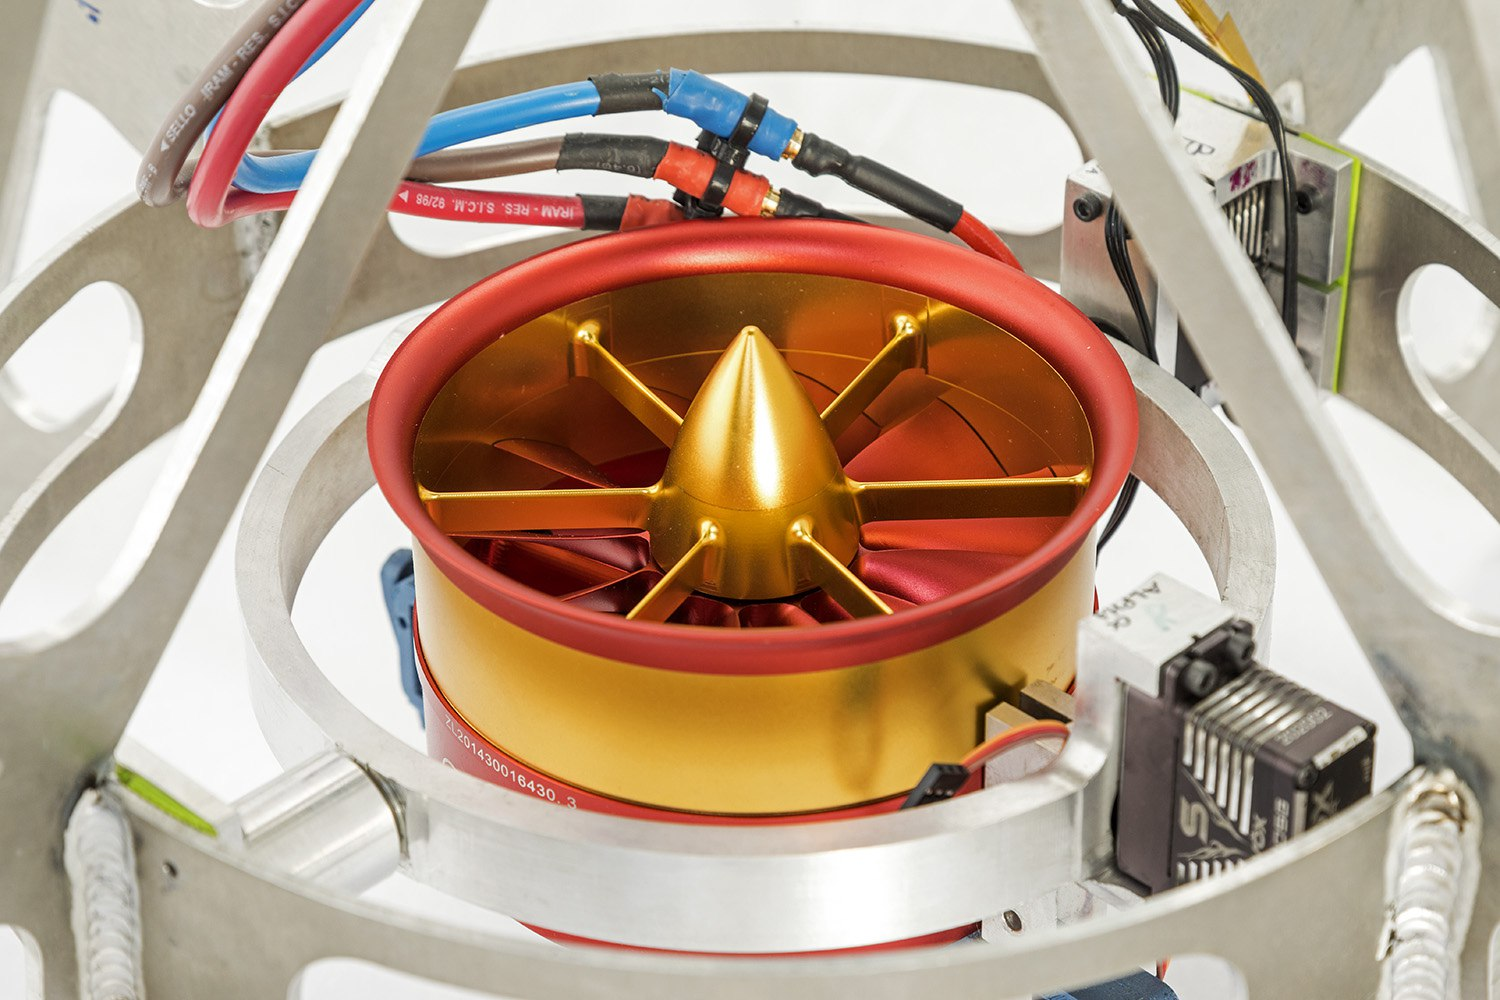
\includegraphics[width=\linewidth]{fig/hq/gimbal_close.jpg}
	\end{figure}
\end{titlepage}

\begin{abstract}
En este documento se encuentran descriptas las secuencias del diseño, simulación, construcción, pruebas, y puesta en marcha de un UAV VTVL. Se evaluaron métodos de propulsión, diseño de fuselaje, software de vuelo, implementación de sistema de control para luego efectuar ensamblaje, y la integración final con testeo en campo. Se logro ensayar el sistema de control a baja escala con el propósito de incorporarlo a un sistema de mayor escala en desarollo paralelo de uso sub-orbital o incluso orbital. 

Se documentan todos los pasos seguidos para llegar al resultado final y se adjuntan los documentos relevantes del desarrollo para su posible replicación incluyendo los planos de cada parte del vehículo, fotos del ensamble, extractos de código, desarrollo de ecuaciones de dinámica de cuerpo rígido y modelos para el control del vehículo mismas usando teoría de control óptimo lineal.

% - Proyecto es punta pie para otros desarrollos mas grandes, i.e: ESA FROG.
% - se propuso un projecto, y se logro
% 	- Como se logro?
% 	- Que nos propusimos?
% 	- No seguimos con las pruebas por el incidente. Nos detuvimos. Llevo a mas mejoras
% 	- Se reescribio todo el codigo, mejora de raiz. Se cambiaron componentes.
% 	- mas protecciones electricas
% 	- El fallo nos mostro el valor del proyecto. Si fuera un VTVL a combustible podria haber sido catastrofico
% 	- problema perdida de control podria generar perdidas en proyectos analogos(seguridad/desarrollos) de la empresa donde se usaba este tipo de tecnologia.
% 	- pruebas de campo

% - Flaps: Se diseño en 3D el soporte de sin tener el EDF en la mano. Cuando llego el EDF nos dimos cuenta que el soporte iba arriba de la parte giratoria.
% 	- Se tuvo que pausar y pensar en un diseño para el soporte que consolide el resto del diseño entero.

% - Queda mucho más para investigar y desarrollar.
% 	- En una proxima iteración podria extenderse el alcance de este desarollo.

\end{abstract}

\newpage
\tableofcontents
\newpage
\printunsrtglossaries
\vfill
\hrule
% \vspace{-1cm}
% \subsection*{Nota del autor}
% Si el documento es abierto desde un lector PDF moderno (Chrome, Adobe Acrobat Reader, entre otros), se podrá navegar el mismo mediante las referencias (haciendo click derecho).

\newpage


\section{Introducción}
El diseño, desarrollo, fabricación, armado, simulación y lanzamiento de cohetes, no es una tarea
sencilla ni repetida en intervalos de cortos de tiempo, al contrario, suelen llevar décadas y una
fuerte inversión para que sean posibles estos logros. El diseño y auge de vehículos VTVL viene
a subsanar estos factores ya que una vez terminada la misión el vehículo se puede reutilizar,
con mínimas intervenciones, y estaría listo para una nueva misión, atacando estos dos puntos principales anteriormente mencionados, el tiempo y el costo. Esto difiere del método convencional donde el vehículo, luego de completar la misión, pasa a formar parte de basura espacial o, en el mejor de los casos, es recuperado del mar como el caso del Space Shuttle. 

\medskip

Un vehículo VTVL es aquel que despega verticalmente (como la mayoría de los cohetes
convencionales) y aterriza verticalmente, por sí solo sin necesidad de ser tripulado, y con el
objeto de completar una misión, esto supone una gran variante de ventajas, como ser una de
las más destacadas el reutilizamiento del vehículo, con todo lo que ello implica, logrando una
optimización de los costos, disminución de huella ecológica, y tiempo de desarrollo para las empresas interesadas. %%

\medskip

Los vehículos VTVL son tan viejos como el primer alunizaje. Traen en si varias ventajas frente a otros vehículos voladores como la gran reducción de espacio necesario para despegar y aterrizar. Esto no es un detalle menor dado que la mayor parte de la superficie terrestre de la tierra no son pistas de aterrizaje si no más bien terreno formado naturalmente.

\medskip

Este documento propone el diseño, simulación, control y fabricación de un vehículo con capacidades VTVL siendo un prototipo de baja escala. 
Este prototipo serviría como punta pie inicial
para vehículos de escala mayor que puedan completar misiones espaciales. Existen varias ventajas de implementar este tipo de tecnología.

\medskip

A baja escala, un vehículo que despega y aterriza por su cuenta, teniendo la capacidad de
superar obstáculos que se presenten, puede ser de gran utilidad en ambientes hostiles para el
ser humano, que esto se logre de manera rápida y efectiva podría ser la diferencia entre el
éxito o no de la misión.
Como ser el transporte de insumos médicos en tiempo real desde que un paciente lo requiere,
en zonas de acceso limitado.

\medskip

En la última década hay un interés renovado en imágenes espaciales. El vehículo podría adquirir imágenes para fines de sistemas de monitoreo y análisis geoespacial como hacen las empresas \textit{Ceres Imaging} y \textit{Satellogic}. %de una situación en la que no se disponga del tiempo suficiente para el accionar convencional a bajas velocidades como ser un helicóptero o un dron.  

\medskip

El vehículo una vez desarrollado y funcionando, puede servir de plataforma para diversos
estudios de fenómenos de dinámica de fluidos, como ser, mediciones aerodinámicas,
investigación del \textit{fuel sloshing} en vehículos con tanques esbeltos.

\medskip

El vehículo provee la capacidad de testear sistemas de control a escala pequeña que en caso de devenir en una falla, el costo total de perdidas seria mucho menor con respecto a un vehículo mas grande con sistemas caros y complejos.  Al tener un sistema de control definido en términos de parámetros del vehículo, se puede escalar para luego ser probado en un vehículo mas grande. Al ser también un sistema más chico y manipulable qué el vehículo de escala grande, tornándose más fácil las pruebas y los problemas de software y hardware de vuelo.

\medskip


Los sistemas de vehículos orbitales tienen sistemas complejos que deben ser testeados en una primera etapa mediante algún ensayo controlado. El vehículo que se desarrolla en el presente documento podría ser usado para tales fines como una plataforma para pruebas como ser el despliegue de una nariz o etapa, comprobación de sensores y actuadores a gran velocidad y con empuje variable.


\section{Estudios}
En lo que se refiere a la construcción del vehículo, el diseño propuesto paso por varias etapas y
decisiones de ingeniería hasta su forma final. Desde su diseño en lápiz y papel hasta la
simulación del CAD con el detalle del ultimo bulón del ensamble para ser cargado al sistema de control en la forma de una matriz de inercia, centro de masa y dinámicas de vuelo, e ir en paralelo retroalimentándose con estos parámetros. En base a esto se realizaron modificaciones sobre el código de control y las simulaciones.


\subsection{Agua como propelente}\label{ssec:propAgua}
El primer prototipo muy distante del diseño final perteneciente a este trabajo, consistía en un
recipiente a presión con agua, abulonado a un chasis, con un cardán y actuadores para poder redirigir el
empuje. 

\medskip

La figura~\ref{fig:bottlerocket} muestra los resultados de una simulación de un vehículo pequeño de aluminio con un recipiente a presión lleno en parte de agua y aire a 200 bar. La simulación considera masa variable y una transición isoentrópica del gas en el recipiente. En el mejor de los casos se llegaba a un tiempo de vuelo cercano a los 4 segundos, que no era adecuado para comprobar el sistema de control en nuestras condiciones. 

Para optimizar este problema se modificaba

\begin{itemize}
    \item Diámetro de la tobera -- más empuje vs. menos tiempo de vuelo controlado
    \item Volumen de agua -- más tiempo de vuelo vs. mayor peso de vehículo
\end{itemize}


\begin{figure}[!ht]
    \centering
    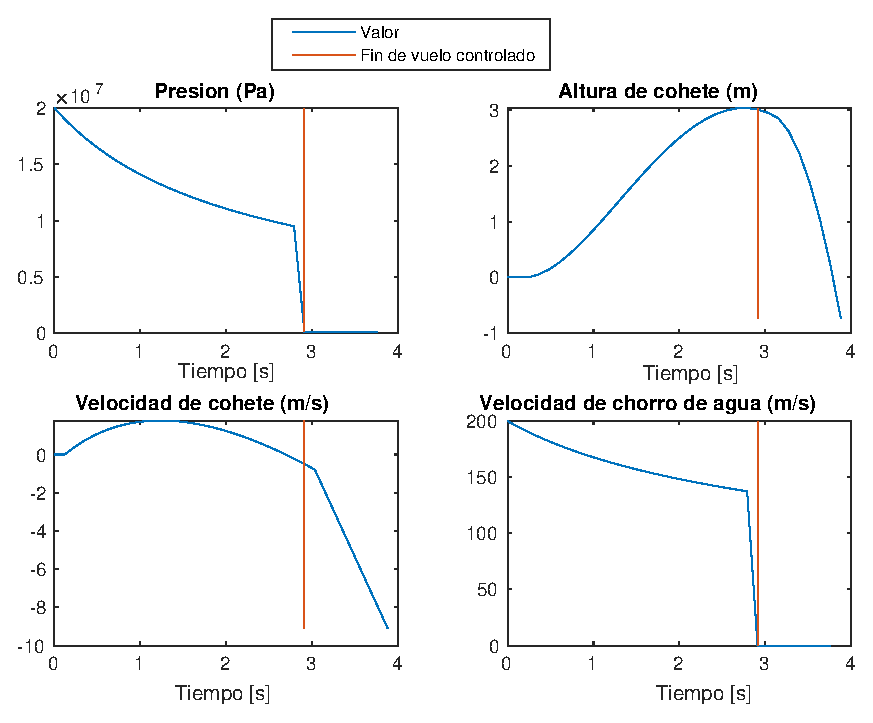
\includegraphics[width=0.8\linewidth]{fig/bottlerocket}
    \caption{Análisis preliminar para un vehículo propulsado por agua a presión. La presión es la del tanque (absoluta). El peso estructural que se utilizó fue de 10kg.}
    \label{fig:bottlerocket}
\end{figure}

Esto representa un vuelo de gran aceleración inicial, de mucha violencia, que dificulta la comprobación de sistemas en el que se tienen que tunear varios los parámetros de control y resolver los problemas de hardware que se vaya presentando. 

\subsection{Turbina a reacción}\label{ssec:turbina}
Se propuso la construcción de una turbina de combustible líquido, como método de propulsión
del vehículo favorable debido al excelente cociente de peso-empuje.

Esta idea se vio descartada por la pandemia que estamos atravesando (COVID19) debido a que
no teníamos acceso al taller de la institución para poder realizar en tiempo y forma el
dispositivo mecánico, que era la primer tarea inmediata a tener en banco de pruebas
asegurando su funcionamiento en optimas condiciones, para luego proseguir con el desarrollo
del vehículo y el sistema de control.


\subsection{Propulsión eléctrica}\label{ssec:propelectrica}


\begin{figure}[htb]
    \centering
    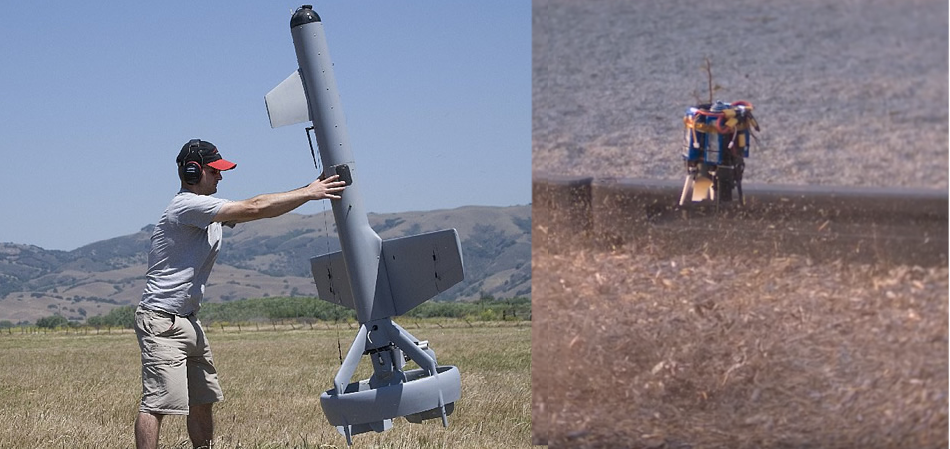
\includegraphics[width=0.8\linewidth]{fig/vbat_icarus.png}
    \caption{Dos vehículos VTVL eléctricos modernos. ``VBat'' (Izq.) y ``\href{https://hackaday.com/2018/08/31/single-rotor-drone-a-thrust-vectoring-monocopter/}{Ikarus}'' (Der.).}
    \label{fig:vbat_icarus}
\end{figure}

Luego de descartar las ideas vistas en~\ref{ssec:propAgua} y~\ref{ssec:turbina} se pasó al análisis de la incorporación de una turbina eléctrica que es un dispositivo ya existente en el mercado, no en nuestro país, pero que podría llegar a importarse teniendo en cuenta la pesificación del valor de los componentes en el exterior y los diversos costos asociados a la entrada al país de los mismos, se contemplo desde ese entonces la financiación privada, que la proveyó LIA Aerospace.\footnote{Agradecemos a \gls{lia} por hacerse cargo de la compra de los componentes faltantes que cayeron fuera del presupuesto necesarios para la fabricación del cohete.} 

Dadas las limitaciones de tiempo y alcance de un proyecto de la universidad se decidió por un diseño compuesto por elementos comercialmente disponibles.\footnote{\textit{Commercial off the shelf} (COTS)}

\medskip

Para lograr estas tareas los vehículos VTVL de baja escala generalmente son propulsados por motores eléctricos, como es el caso del proyecto FROG de la ESA.\todo{AGREGAR CITA}

\medskip

Los vehículos VTVL eléctricos son propulsados por hélices en su mayoría y constan casi siempre de 3 o más propulsores en un arreglo simétrico y plano. Recientemente hay un interés por la construcción de vehículos de una sola hélice por la buena relación empuje--peso que tienen. Sin embargo, estos vehículos no vienen sin sus complicaciones: 

\begin{itemize}
    \item La rotación dada al aire por la hélice causa un momento en el eje de propulsión que puede ser contrarrestado en vehículos multirrotores.
    \item Inclinar al rotor durante su funcionamiento causa una fuerza perpendicular a la dirección de inclinación conocido como el efecto giroscópico. 
\end{itemize}

El primer punto puede ser mitigado agregando álabes a la salida del chorro para enderezar el flujo y contrarrestar la rotación. El segundo punto se resuelve conociendo las ecuaciones de momento angular y controlando actuadores con un sistema de control a lazo cerrado. Los sistemas vistos en la figura~\ref{fig:vbat_icarus} suelen tener la particularidad de poder ser representados con relativa facilidad usando un solo marco de referencia sobre el vehículo para calcular las ecuaciones de momento angular.

\medskip

Existen placas pre-programadas para vehículos multirrotores, pero en el caso de vehículos monorrotores de hélice fija se precisa re-programar la placa para compensar por el efecto giroscópico y agregar dinámica de álabes ya que no hay software disponible aún para esta configuración. En el caso de tener una hélice móvil se suma un nivel de complejidad agregada debido al despeje de las ecuaciones de momento angular (ver sección~\ref{sec:ecuacionesRigid}). Al momento de escribir este documento aún no hay desarrollo disponible de carácter público para esta configuración.

\null\newpage
\clearpage

\section{Diseño}

En el marco de este proyecto, es de interés el diseño mecánico del mecanismo de control semejante un vehículo propulsado por combustión externa. Estos últimos suelen ser dirigidos por toberas montadas sobre un cardán. En el caso de un vehículo eléctrico de una hélice se tendría que montar el sistema de propulsión centrado en un gimbal para no obstruir el flujo.

\subsection{Selección de propulsador}

Existen diversas maneras de impulsar un vehículo de forma eléctrica. Luego de un cuidadoso estudio y discusión de ingeniería se decidió optar por un \gls{edf}, quien juega un rol central en el diseño pues es lo que se intenta controlar para llevar a cabo la navegación y guiado. Se analizo
ir por un EDF de aluminio, por una cuestión de durabilidad, relación empuje-peso, reducir probabilidad de fallas y roturas en sucesivos experimentos. 
Los EDF de aluminio solo se consiguen en el exterior y su precio es en dolares\footnote{El cambio de divisas es desfavorable para el lugar donde se desarrolla este proyecto.}. Esto trae varios inconvenientes en lo referente al presupuesto acotado, logística, compra y obtención. Los EDF
disponibles de plástico tienen una relación de empuje-diámetro mucho menor con respecto a
los de aluminio. Cabe destacar que el costo de un EDF de plástico y un EDF de aluminio son cercanos para diámetros similares.

\todo{Hablar del bucle}

\subsection{Diseño de la mecánica}

Para el diseño del gimbal se propuso una distribución de los mecanismos de actuación con
servos concéntricos a los ejes de rotación. Para evitar de esta manera complejidad de
mecanismos, cantidad de piezas de conexión entre servo y ejes, manufactura de mecanismos,
uniones rotoides, y obtener así un mapeo lineal del ángulo de actuación. El único intermediario
es el rodamiento que como se dispuso en la configuración ocupa el mínimo lugar posible justo
por encima de la estría del servo y se lleva las cargas.
Este mecanismo viene con la desventaja de una reducción de la resolución del ángulo de actuación comparado a un sistema actuado por un mecanismo biela-manivela.

\medskip

El material seleccionado para la fabricación del gimbal fue aluminio serie siete mil calidad
aeroespacial. Esta construido de una sola pieza, siendo el elemento que se lleva las tensiones
en todo momento en variabilidad de ángulos hacia el fuselaje, por ello la decisión de ser de la
serie de mayor resistencia mecánica de los aluminios comerciales.

\medskip

Los rodamientos seleccionados son de dimensiones 18mm exterior, 10mm interior y 7mm de espesor,
elegidos de esta manera por una cuestión de espacio para poder pasar la estría de los
servomotores por dentro, dejando un espesor de la pared del estriado de 2.5mm,
para evitar fisuras y hacer posible la manufactura de la pieza. La forma de generar el estriado
interno, es la de indentar con un patrón sobre un agujero previo de diámetro medio a los
valores máximos y mínimos de las crestas y valles de la estría. Esta operación debe hacerse con
el material en bruto para no arruinar las tolerancias que necesitan los rodamientos. Los
rodamientos se montarían clavados, minimizando el peso al no agregar seguers ni tapas con
bulones.

\medskip 

Los ejes del gimbal estarían en disposición simplemente apoyada y de forma axisimétrica para prevenir perturbaciones dinámicas por desbalanceo.

\medskip

Con respecto al fuselaje, al inicio se pensó una envolvente cilíndrica para el anillo externo del
gimbal. Luego se diseñó un desarrollo reticulado optimizado, se pasó por diferentes modelos e
ideas, hasta que se combinaron varios puntos fuertes de cada idea. La envolvente del gimbal se fabrica de forma rolada y optimizada en peso a raíz de
una planchuela de aluminio vaciada y luego generando su forma cilíndrica.\footnote{Contiene al
anillo del gimbal.} Esto distribuye las masas de manera más favorable con menos espacio
ocupado (dinámica-peso). Aguas arriba del gimbal se opto por un chasis tubular, con diversos
vaciados, que mediante flejes puede soportar cada elemento que se acopla al cohete por
medio de uniones abulonadas. Permitiendo mediante sus aberturas el acceso a cada
componente del vehículo, proporcionando, además, una renovación del aire para una
evacuación del calor generado, y un flujo abundante hacia la admisión del EDF.

\medskip

De la manera que se construye el gimbal puede entregar una rotación entera sin hacer contacto con la estructura. Se elige esta configuración por posibles desviaciones del proyecto en el
futuro, calculamos que utilizaremos menos de 20$^\circ$ de rotación de cada eje de gimbal ($\pm$10$^\circ$).

\subsection{Posición de baterías}

La la decisión de donde posicionar las baterías surgía de querer simular un vehículo semejante a los VTVL de la industria aeroespacial y también la posibilidad de tener una inercia favorable para los margenes de estabilidad. Estos dos últimos puntos sugieren que la posición ideal para las baterías es arriba de todo. Esto haría que el punto alrededor del cual se linealizó las ecuaciones de movimiento sea más estable. Luego de una conversación con Pablo Cossutta, un ingeniero electrónico especialista en sistemas de potencia, se optó por la configuración encontrada en el documento. Las baterías se encuentran cerca del EDF para alejar las líneas de potencia trifásica correspondientes al motor brushlesss de lo que es la electrónica digital. Al inestabilizar el punto de operación se obtiene una mejora en la respuesta ante actuaciones permitiendo una corrección de trayectoria más rápida.\footnote{Este resultado es deseado cuando se desea tener mejor rendimiento por ángulo de actuación, como sucede con los \textit{aviones caza} que utilizan este fenómeno a conveniencia.}


\subsection{Selección de servos} \label{ssec:servoSeleccion}
\newcommand{\micro}{\ensuremath{\mu}}
\newcommand{\grad}{\ensuremath{^\circ}}
Para obtener una buena respuesta del vehículo ante actuaciones se debe acotar la resolución necesaria. Según \cite{castillo2018efectos}, la resolución angular de un servo analógico está dada por


\[
R_p = \frac{\theta \cdot T_D}{PW}  
\]

donde $\theta$ es el angulo de barrido del servo (especificado por el fabricante), $T_D$ es el tiempo muerto y $PW$ es el ancho de pulso operativo. 

El servo seleccionado es el SC1258TG. Tiene las siguientes especificaciones

\begin{itemize}
    \item Tiempo muerto (\textit{deadband}) 3\micro s
    \item Rango de ancho de pulso mínimo y máximo 800-2100\micro s
    \item Posición neutra 1500\micro s
    \item Ángulo de barrido operativo 100\grad (para 1000-2000\micro s)
    \item Velocidad 1,05 rad/s
    \item Controlador digital
\end{itemize}

Se tiene entonces una resolución mínima de 0,3\grad~ con un ancho de pulso de 2000\micro s. Esta cuenta cede la resolución para un servo analógico, en el caso de tener un servo digital se toma el límite superior entre este valor y la resolución del controlador digital. Como el fabricante no especifica el controlador utilizado, se supone el peor de los casos: un controlador de 8 bits. Este caso tiene una resolución de 0,4\grad~.

Esta resolución es alimentada como parámetro de actuación en las simulaciones.


\subsection{Selección de electrónica}

Se pasó por varias etapas hasta llegar a la decisión final del controlador. Se empezó planteando la utilización de una Raspberry Pi 4B+ para controlar los actuadores con PWM. Esta configuración requiriría el diseño de una placa ad-hoc para desacoplar galvánicamente la Raspberry del controlador de velocidad del EDF (\gls{esc})

El \textbf{controlador} a usar es el ARM Cortex-A72 que sería comprado en el paquete comercial (\gls{soc}) conocido como \textit{Raspberry Pi 4B+}. El producto provee salidas para los siguientes usos

\begin{itemize}
    \item \glsxtrshort{uart}
    \item \glsxtrshort{spi}
    \item \glsxtrshort{i2c}
    \item \glsxtrshort{gpio}
\end{itemize}

El controlador ira montado sobre una placa cuyo desarrollo pertenece a LIA Aerospace denominada \textbf{LIA-Board}. Esta placa hace interfaz con el controlador mediante el GPIO header del \gls{soc}. Esto le permite al controlador acceder a los periféricos y salidas disponibles del LIA-Board que controlaran los actuadores y leerán los sensores.


\subsection{Contexto de pandemia}
Las medidas tomadas durante la pandemia por el gobierno fueron muy estrictas e influenció a todo tipo de acción que se quiso tomar. Durante el primer año de pandemia no nos pudimos reunir físicamente para discutir ideas de diseño, lo cual dificultó el avance físico del proyecto como así también la toma de decisiones y la comunicación entre partes, crucial en el inicio de todos proyectos de ingeniería.

\medskip

Una de las mayores complicaciones que se tuvo fue la compra de
componentes, además de la fabricación, que se vio afectada, por las políticas cambiantes de
nuestro país con respecto a la compra y la entrada de productos importados a suelo argentino.
Incluso la compra y llegada de los productos fue un motivo de festejo luego de un tortuoso
trayecto.




\null\newpage
\clearpage

\section{Análisis estructural}\label{sec:fea}

El diseño de este prototipo fue ampliamente debatido. Para llegar a buen puerto con las decisiones de ingeniería, lo que se utilizó fue la herramienta de elementos finitos. Más allá del buen planteo del diseño inicial, necesario para poder optimizar luego el prototipo. Un diseño malo de entrada, no hay elemento finito que lo arregle. Por esto fue crucial en base a la experiencia adquirida en estos años de estudios poder plantear un diseño inicial acorde a las necesidades en distintas circunstancias de prueba, para luego poder iterarlo. Obteniendo un coeficiente de peso y resistencia que nos sirva para poder probar el sistema de vuelo en un vehículo liviano, porque el empuje era un factor limitante, que sobreviva a los distintos escenarios y pruebas de maniobras. Para poder llegar a la finalización del proyecto en condiciones mecánicas funcionales, es decir, poder tunear de manera correcta el sistema de control sin destrozar el prototipo en el camino.

\medskip

El fuselaje fue la parte mecánica con mayor cantidad de iteraciones, se pasó por distintos prototipos. Cada uno de ellos fue pensado en el diseño intentando llevar a su geometría a la forma más eficiente pensando cómo viajaban las cargas en distintas condiciones. Para la condición de vuelo, las cargas eran el empuje del EDF y el peso  principalmente, y combinadas con los cambios bruscos de aceleración, para este caso se encontró que las limitaciones eran las geométricas. Se continuó con el modelado de la estructura imponiéndole una fuerza en la parte superior y como parámetro de decisión se utilizó el criterio que suele utilizarse en el ámbito aeroespacial que es ponerle a distintas estructuras 1 N de fuerza y ver entre ellas cuál es la más eficiente para este caso de carga. Para luego decidir entre estos prototipos y proponer una carga de prueba para comprobar que no se estaba en fluencia. Se detectó que el aterrizaje era la peor condición, así que se diseñó y modeló para este caso. Siendo el peor escenario posible caer con solo una pata a impacto y de costado, pero en el segundo rebote, es decir tocar el piso a impacto y luego al girar que soporte todo el peso del vehículo sin plastificar de costado, multiplicado por 1,4 que fue el factor de seguridad elegido (paper referencia nasa). Se decidió corroborar a fluencia la carga lateral mencionada en la pata y en el extremo superior con una carga de 100 N que resulta de multiplicar 7 Kg * 1,4 dividirlo por la gravedad y redondearlo al entero superior. En la finalización del proyecto se encontró que esta predicción fue correcta.

\medskip

Se hicieron varios modelos de distintos prototipos de fuselajes con elementos finitos, solo se muestran aquellos que nos agregaron información relevante al desarrollo de este proyecto, y las discusiones interesantes de ingeniería que en fuertes debates pudieron lograr el prototipo final .En total se han planteado 11 conjuntos de cad distintos con fuselajes distintos para luego ser modelados.

\null\newpage
\clearpage

\subsection{Modelo y simulación propuesta tipo jaula}
\begin{figure}[htb]
    \centering
    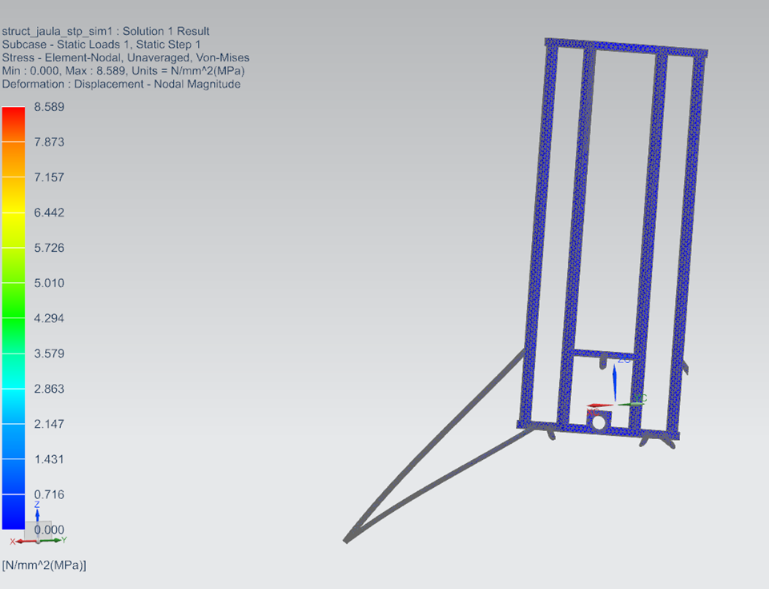
\includegraphics[width=\linewidth]{fig/fea/jaula.png}
    \caption{Modelado inicial estructura esfuerzos para carga de 1N estático en las patas dirección normal al suelo modelo de fuselaje tipo jaula.}
    \label{fig:fea/jaula}
\end{figure}

\begin{figure}[htb]
    \centering
    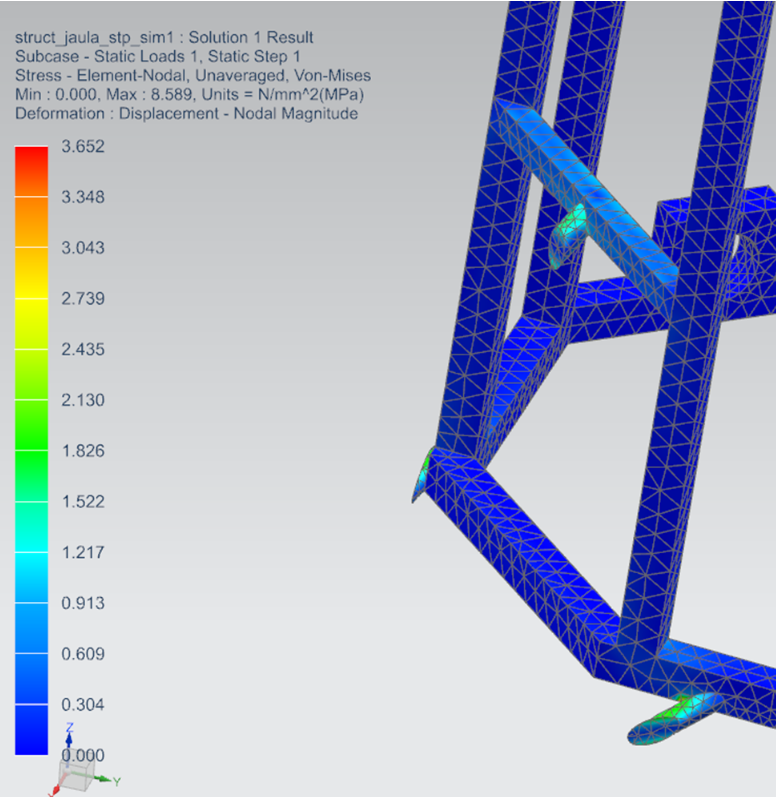
\includegraphics[width=\linewidth]{fig/fea/jaula2.png}
    \caption{Esfuerzos para carga de 1N estático para misma condición de la figura anterior pero solo vista de esfuerzos de la parte superior quitando las patas.}
    \label{fig:fea/jaula2}
\end{figure}

\null\newpage
\clearpage

\subsection{Modelo y simulación del fuselaje tubo y placas vaciadas}

\begin{figure}[htb]
    \centering
    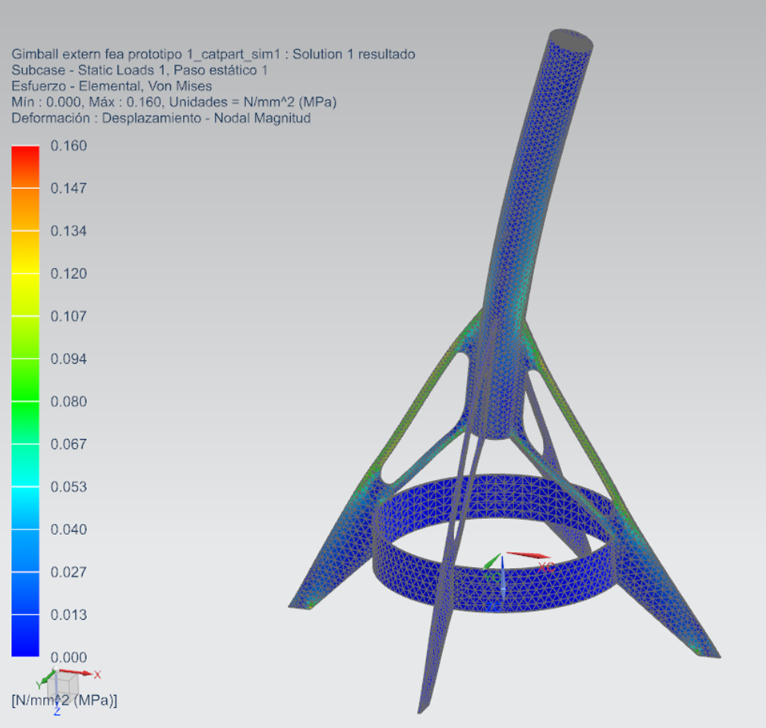
\includegraphics[width=\linewidth]{fig/fea/tuboplaca1.png}
    \caption{Modelo tubo y placas esfuerzo elemental para carga superior de 1 N en dirección planar al suelo.}
    \label{fig:fea/tuboplaca1}
\end{figure}

\begin{figure}[htb]
    \centering
    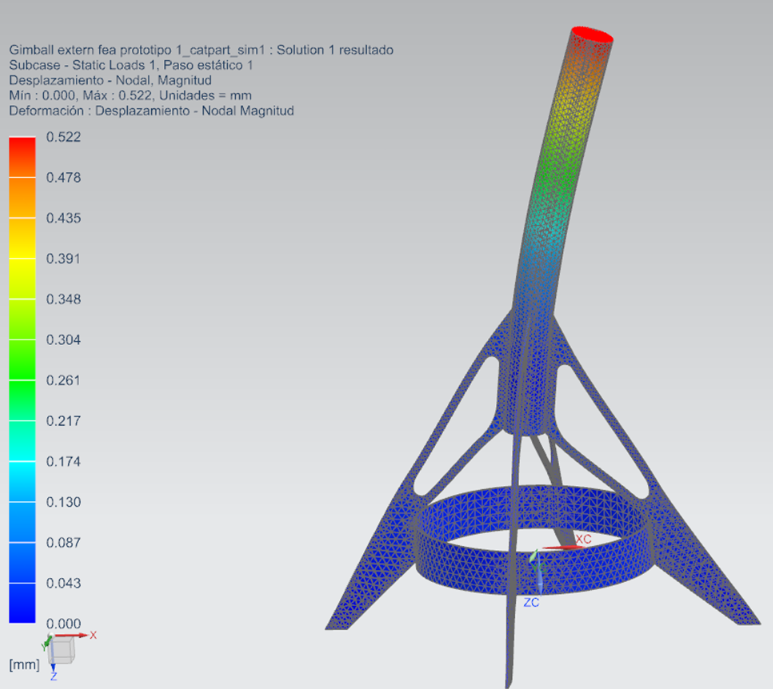
\includegraphics[width=\linewidth]{fig/fea/tuboplaca2.png}
    \caption{Modelo tubo y placas desplazamiento elemental para carga superior de 100 N en dirección planar al suelo.}
    \label{fig:fea/tuboplaca1}
\end{figure}

\begin{figure}[htb]
    \centering
    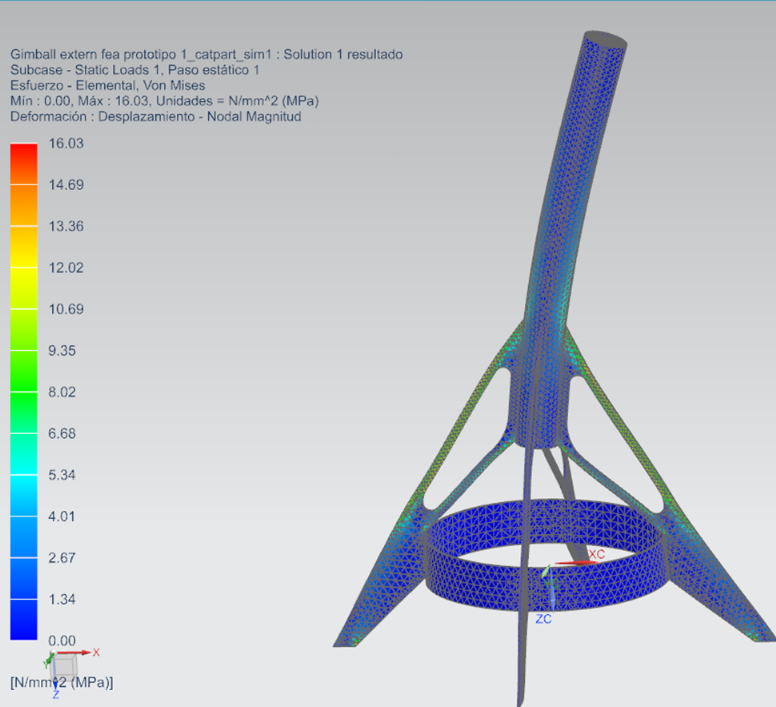
\includegraphics[width=\linewidth]{fig/fea/tuboplaca3.png}
    \caption{Modelo tubo y placas esfuerzo elemental para carga superior de 100 N en dirección planar al suelo.}
    \label{fig:fea/tuboplaca3}
\end{figure}

\begin{figure}[htb]
    \centering
    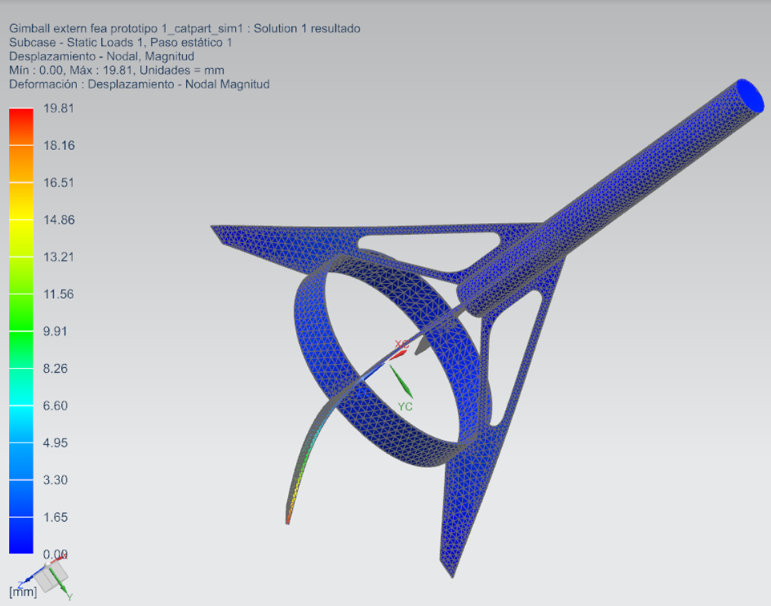
\includegraphics[width=\linewidth]{fig/fea/tuboplaca4.png}
    \caption{Modelo tubo y placas deformación en una de sus patas con una carga de 100N en dirección normal a la superficie de una de sus patas.}
    \label{fig:fea/tuboplaca4}
\end{figure}

\begin{figure}[htb]
    \centering
    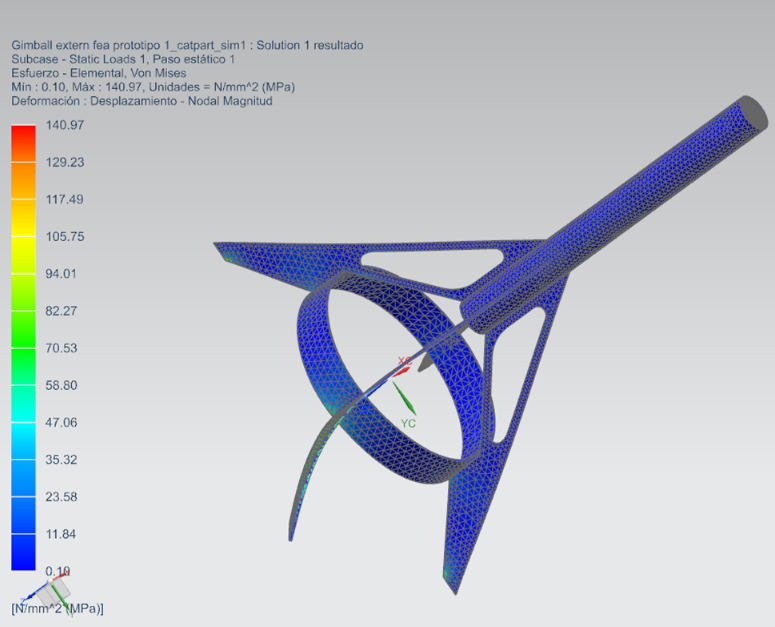
\includegraphics[width=\linewidth]{fig/fea/tuboplaca5.png}
    \caption{Modelo tubo y placas esfuerzo en una de sus patas con una carga de 100N en dirección normal a la superficie de una de sus patas.}
    \label{fig:fea/tuboplaca5}
\end{figure}

\begin{figure}[htb]
    \centering
    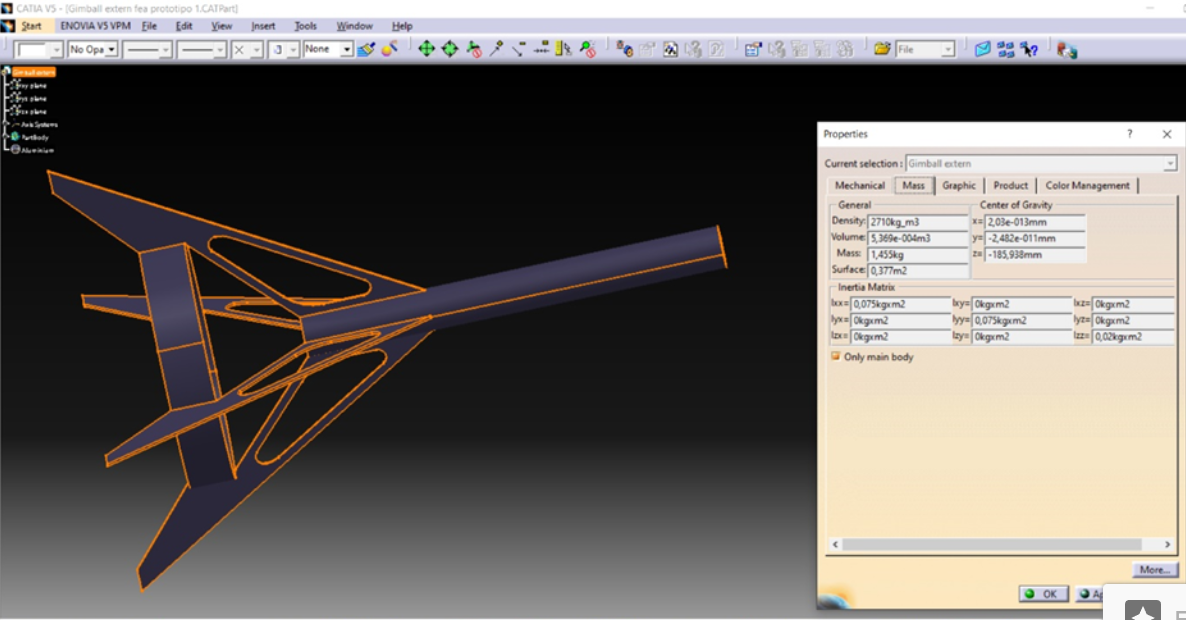
\includegraphics[width=\linewidth]{fig/fea/inercias}
    \caption{Peso e inercias del prototipo analizado.}
    \label{fig:fea/tuboplacainercias}
\end{figure}

\null\newpage
\clearpage

\subsection{Iteración del modelo y simulación en la que se definió la geometría final de las placas que componen las patas}

\begin{figure}[htb]
    \centering
    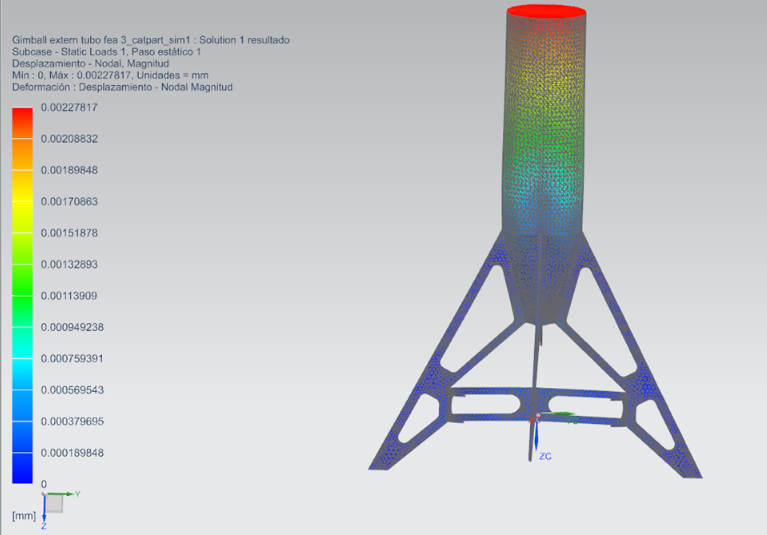
\includegraphics[width=\linewidth]{fig/fea/patas1.png}
    \caption{Modelo tubo y placas iteración $n$ desplazamiento para carga superior 1 N en dirección planar al suelo.}
    \label{fig:fea/patas1}
\end{figure}

\begin{figure}[htb]
    \centering
    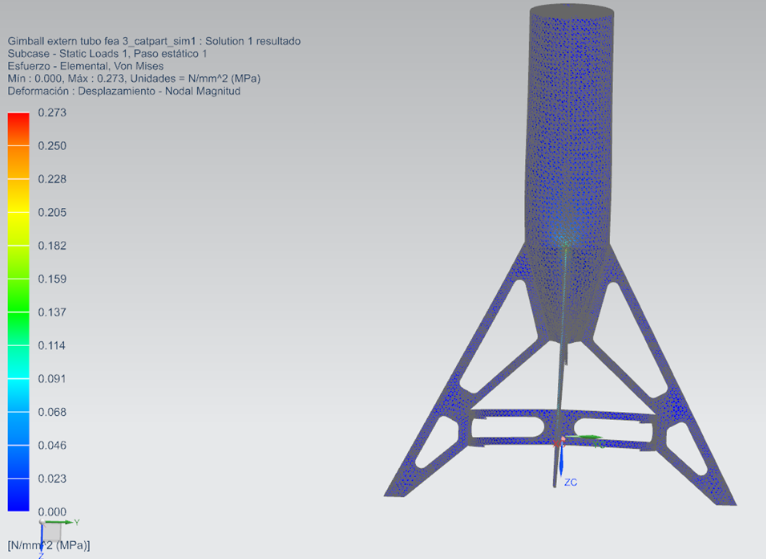
\includegraphics[width=\linewidth]{fig/fea/patas2.png}
    \caption{Modelo tubo y placas iteración $n$ esfuerzos elementales para carga superior 1 N en dirección planar al suelo.}
    \label{fig:fea/patas2}
\end{figure}

\begin{figure}[htb]
    \centering
    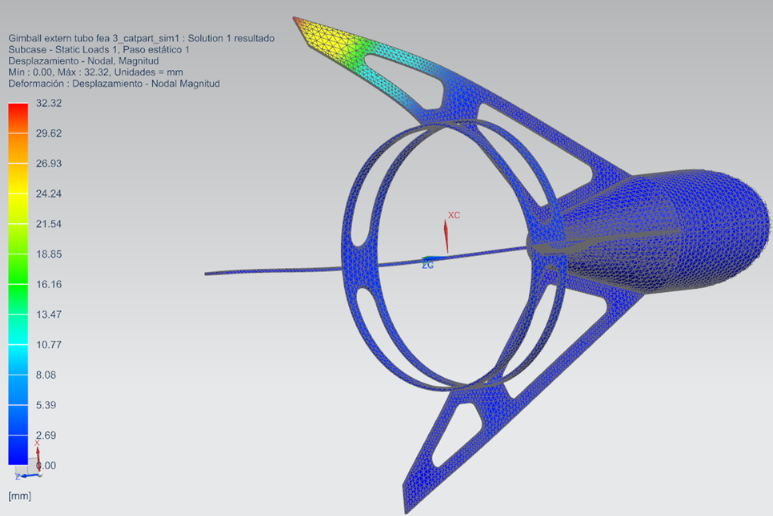
\includegraphics[width=\linewidth]{fig/fea/patas3.png}
    \caption{Modelo tubo y placas iteración $n$ desplazamientos con cargas de 100N en dirección normal a la superficie de una de sus patas.}
    \label{fig:fea/patas3}
\end{figure}


\begin{figure}[htb]
    \centering
    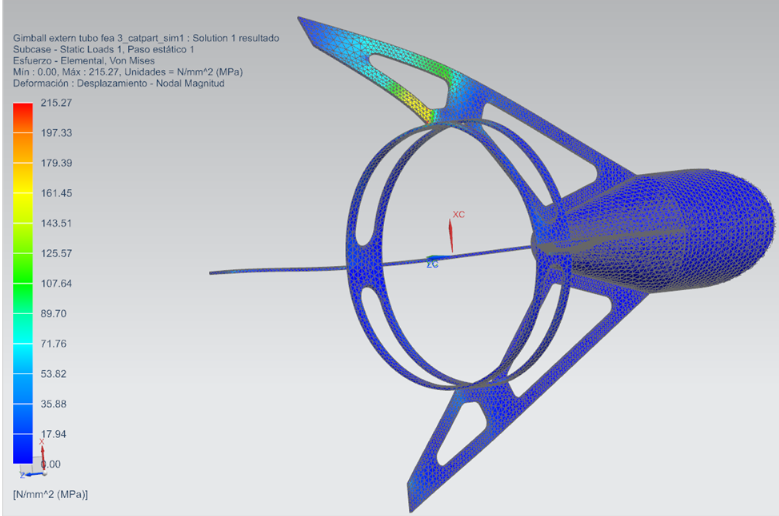
\includegraphics[width=\linewidth]{fig/fea/patas4.png}
    \caption{Modelo tubo y placas iteración $n$ esfuerzos elementales con carga de 100N en dirección normal a la superficie de una de sus patas.}
    \label{fig:fea/patas4}
\end{figure}

\begin{figure}[htb]
    \centering
    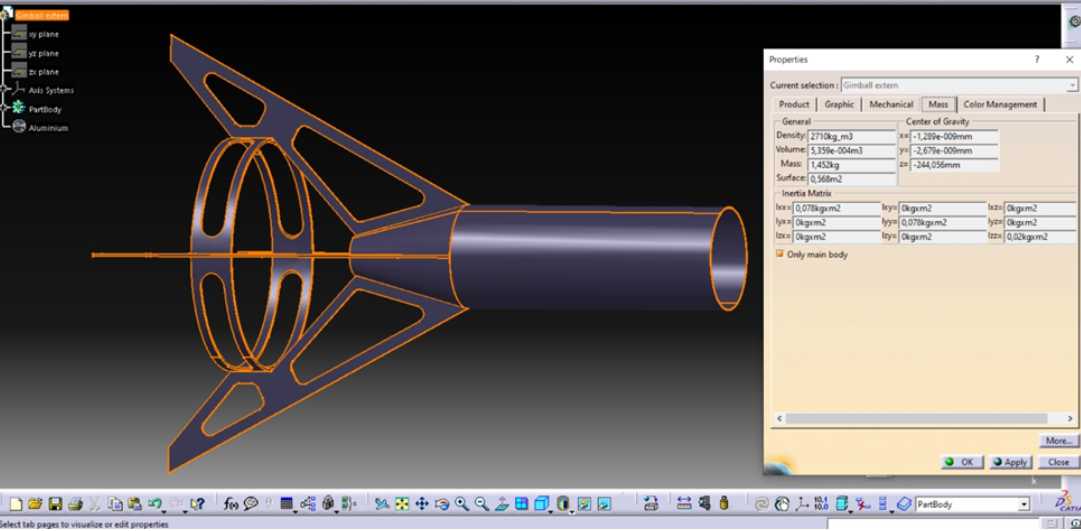
\includegraphics[width=\linewidth]{fig/fea/inerciaspatas.png}
    \caption{Peso e inercias del prototipo analizado.}
    \label{fig:fea/patas4}
\end{figure}

\begin{figure}[htb]
    \centering
    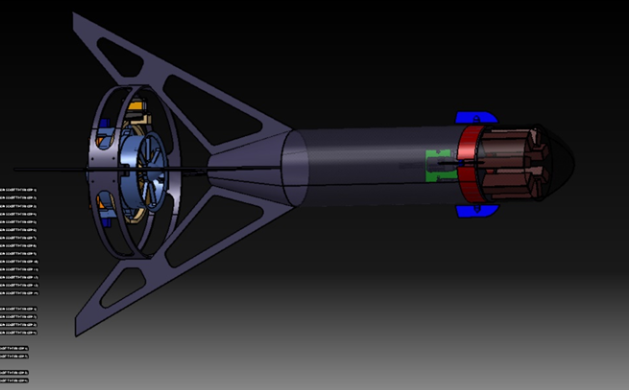
\includegraphics[width=\linewidth]{fig/fea/imagenpatas.png}
    \caption{Imagen del conjunto del prototipo del prototipo analizado.}
    \label{fig:fea/imagenpatas}
\end{figure}

Se comprobó que las patas aguantaron las cargas de diseño para su peor condición con factor de seguridad mayor a 1.4.

Como se vio que la estructura tubular estaba sobredimensionada para ser portadora de los componentes electrónicos, sin más análisis se procedió al vaciado para poder acceder a la electrónica. Se optó por una cuestión de simplicidad y avance con los tiempos de manufactura de prescindir del cono invertido superior, quedando tubular el diseño final del fuselaje. 



\null\newpage
\clearpage

\section{BOM, despiece y figuras del diseño mecánico}

\subsection{Diseño final - BOM y despiece}
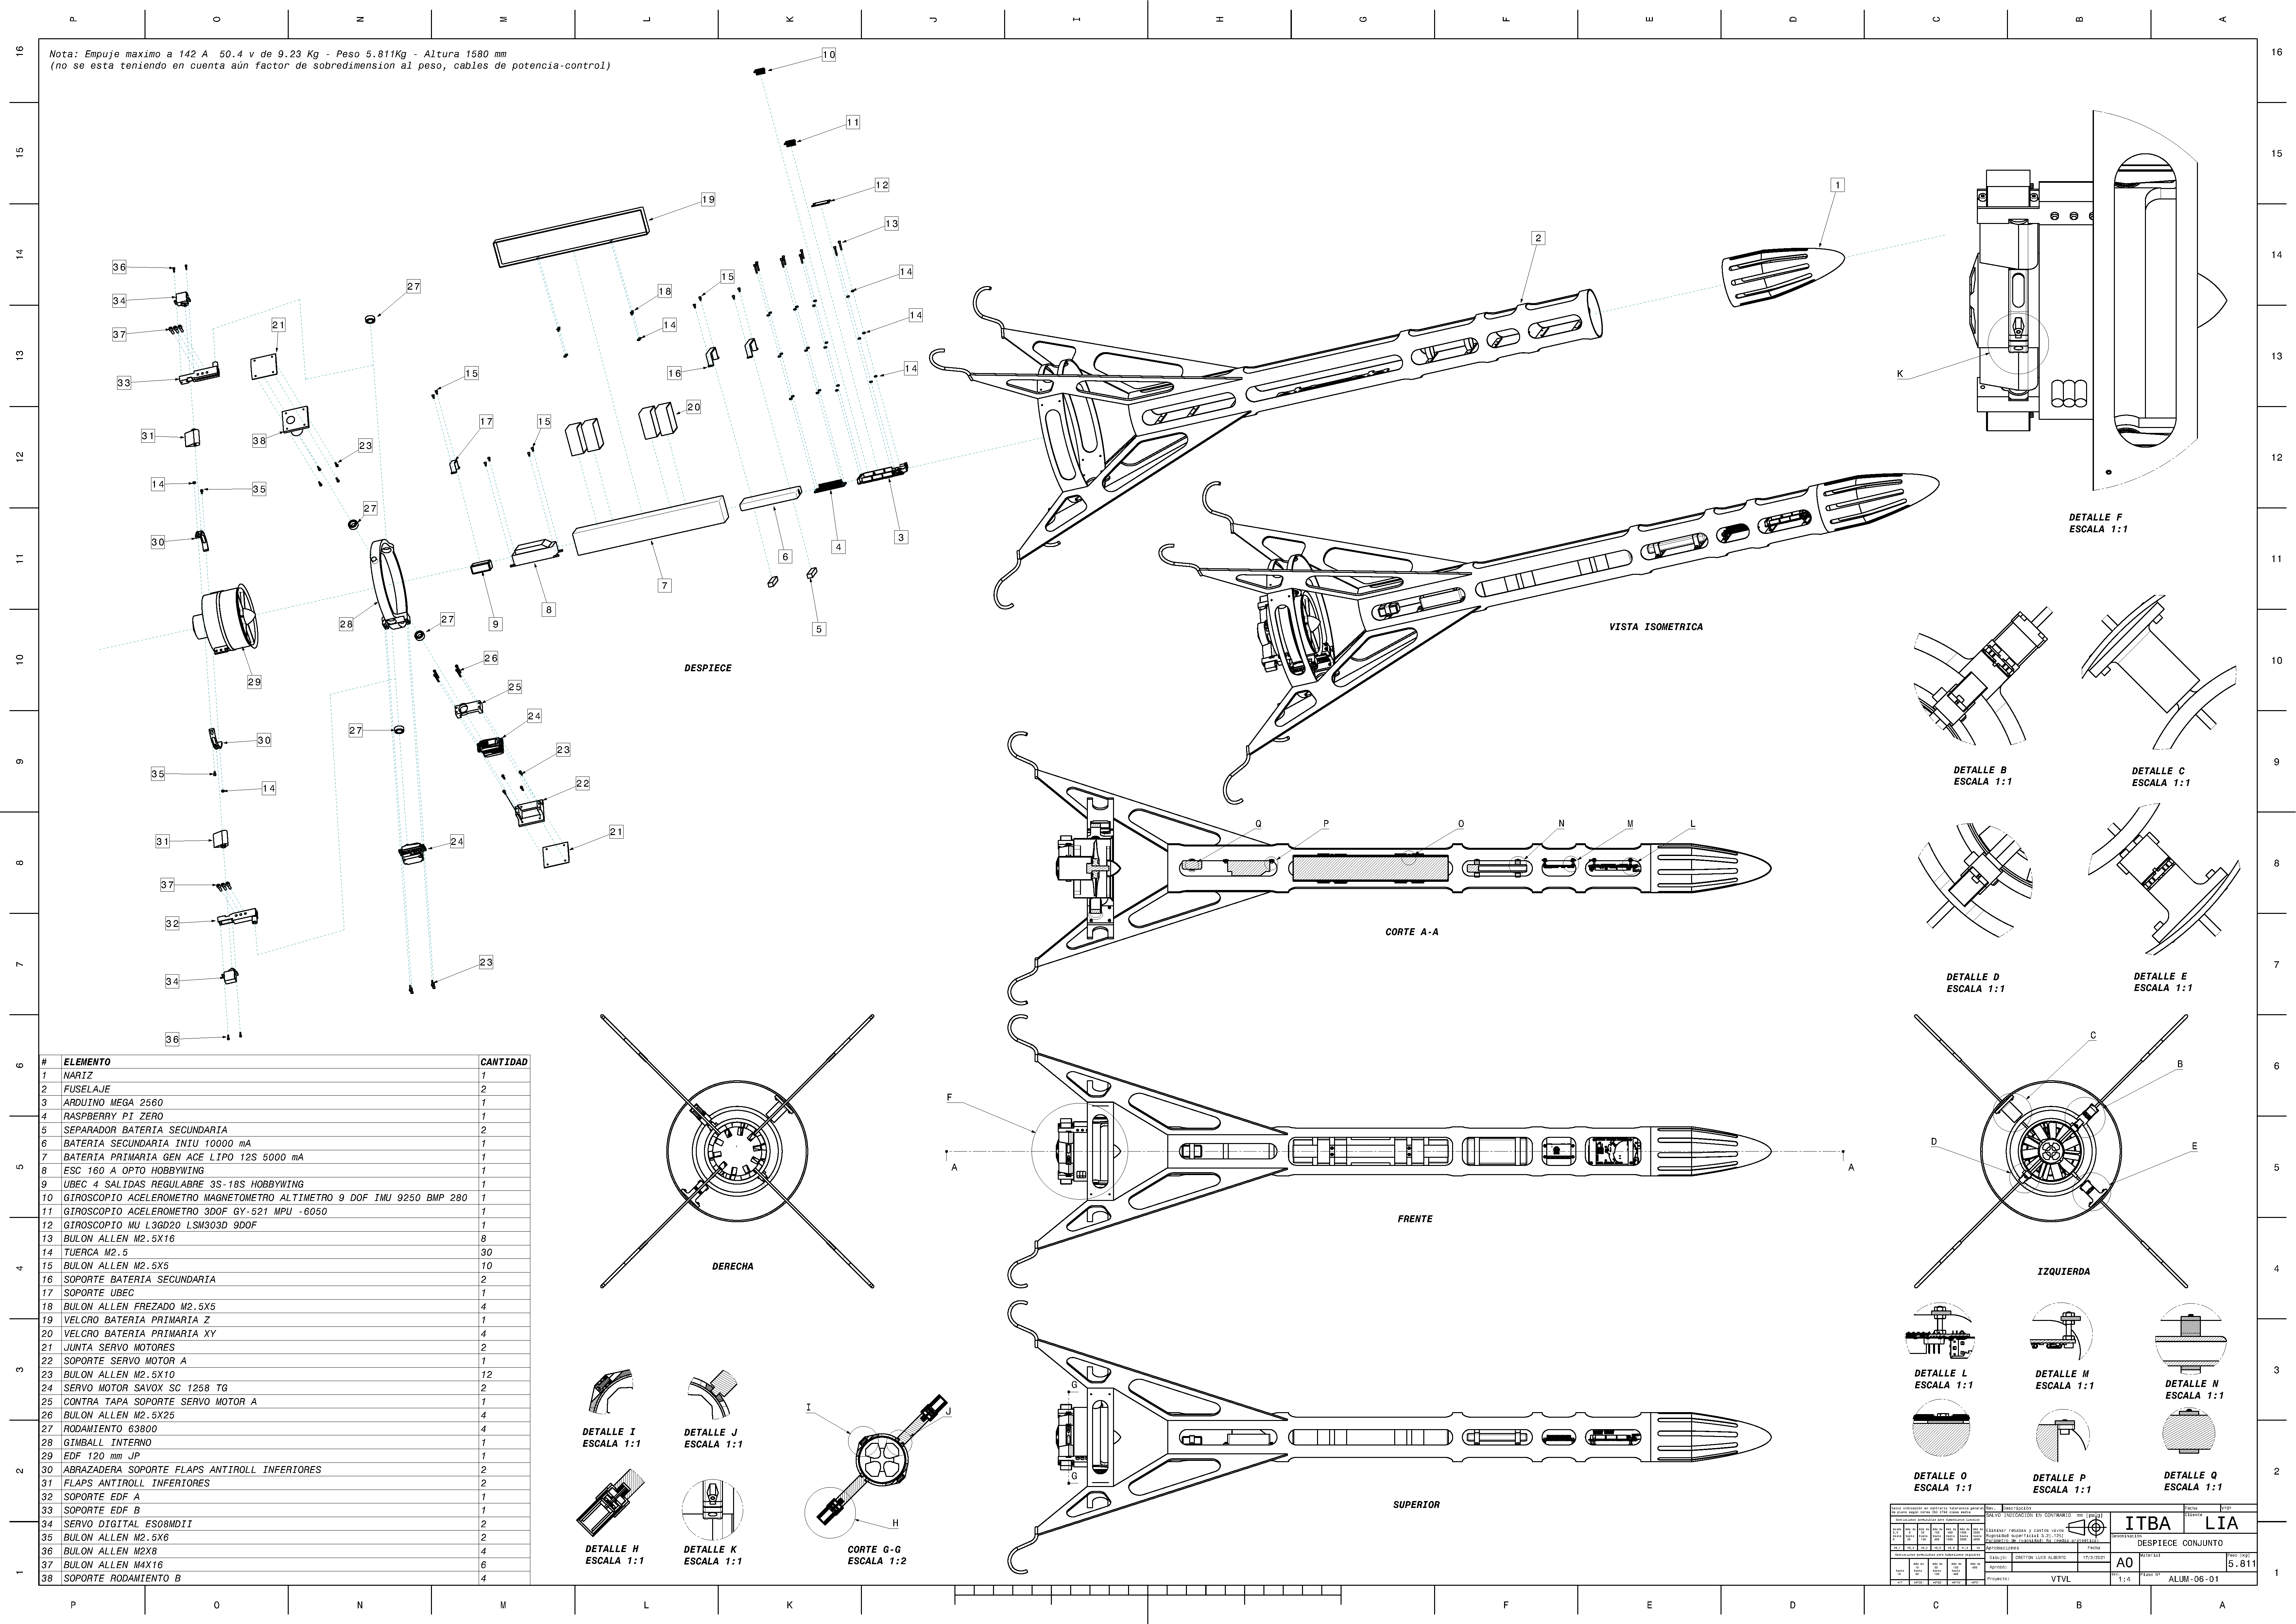
\includepdf[angle=90]{pdf/cad/ALUM-06-01} % Vista explotada del diseño final


\subsection{Diseño final - Imágenes}
% \todo{Si podemos quitar imagenes mejor. Yo personalmente no agregaría mas imagenes a no ser que agreguen valor. No agregaria las dos imagenes del anexo solo asi todo queda junto. }
\begin{figure}[htb]
    \centering
    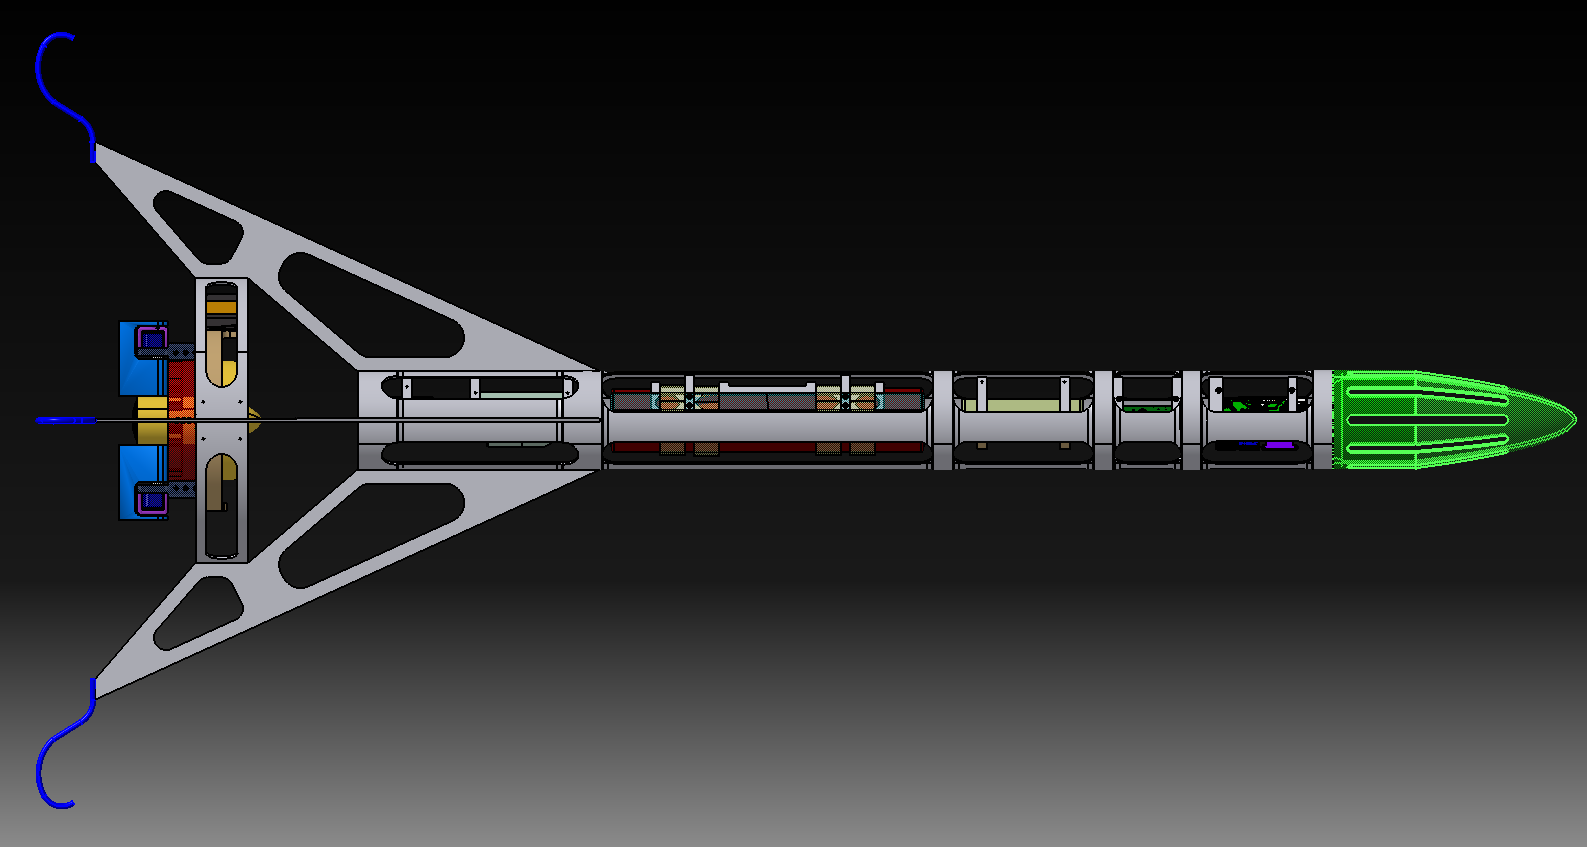
\includegraphics[height=0.3\pdfpageheight,angle=90]{fig/design/v6}
    \caption{Prototipo final, vista de frente, batería principal en el núcleo, incorporación de batería secundaria, aviónica en la parte superior, nariz aerodinámica, sistema anti-rolido en la parte inferior por derivación del flujo, patas y fuselaje vaciado, sistema de suspensión elástico.}
    \label{fig:design/v6}
\end{figure}

\begin{figure}[htb]
    \centering
    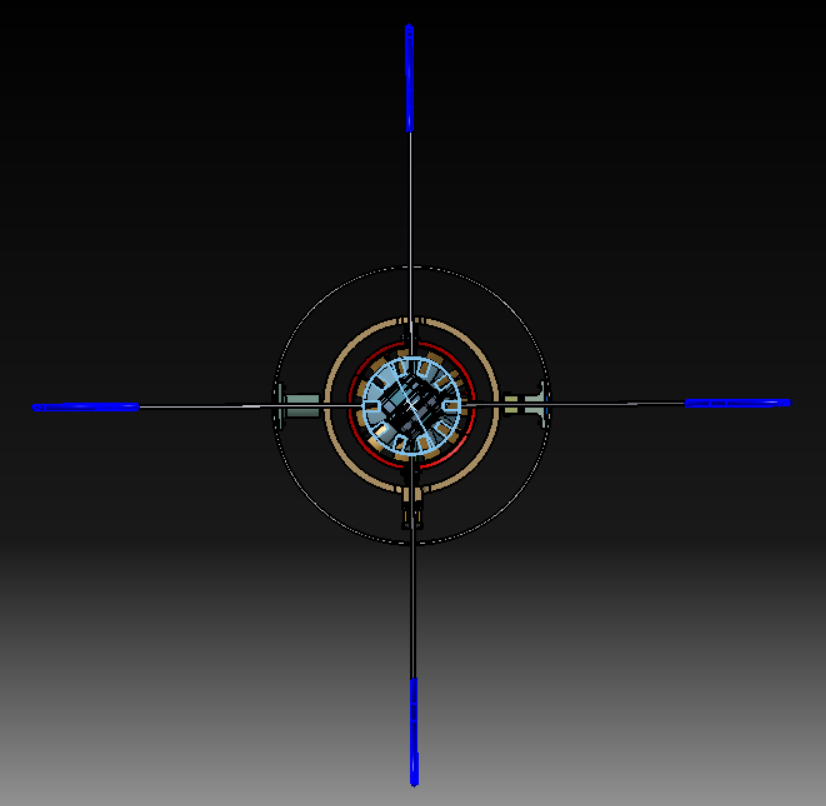
\includegraphics[height=0.3\pdfpageheight]{fig/design/v6_1}
    \caption{Prototipo final, vista superior.}
    \label{fig:design/v6_1}
\end{figure}


\begin{figure}[htb]
    \centering
    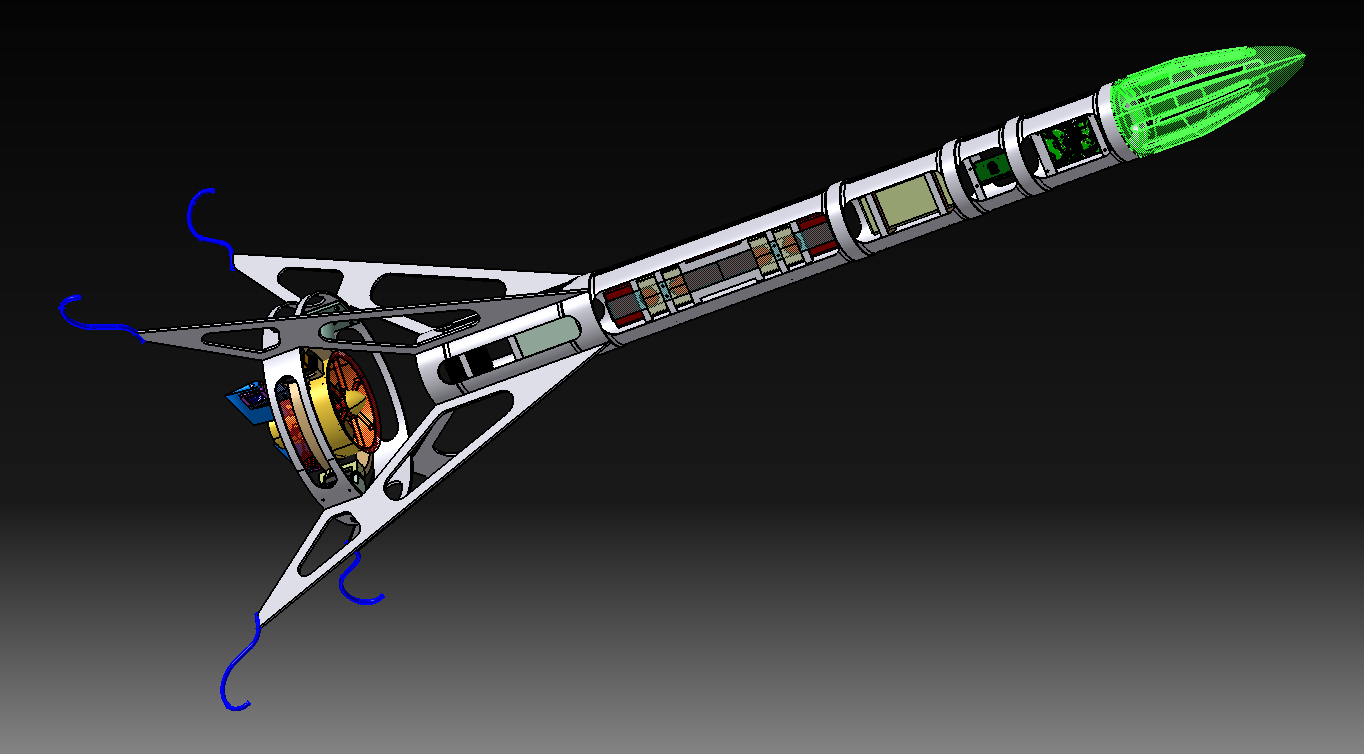
\includegraphics[height=0.3\pdfpageheight]{fig/design/v6_2}
    \caption{Prototipo final vista isométrica axonométrica.}
    \label{fig:design/v6_2}
\end{figure}



\begin{figure}[htb]
    \centering
    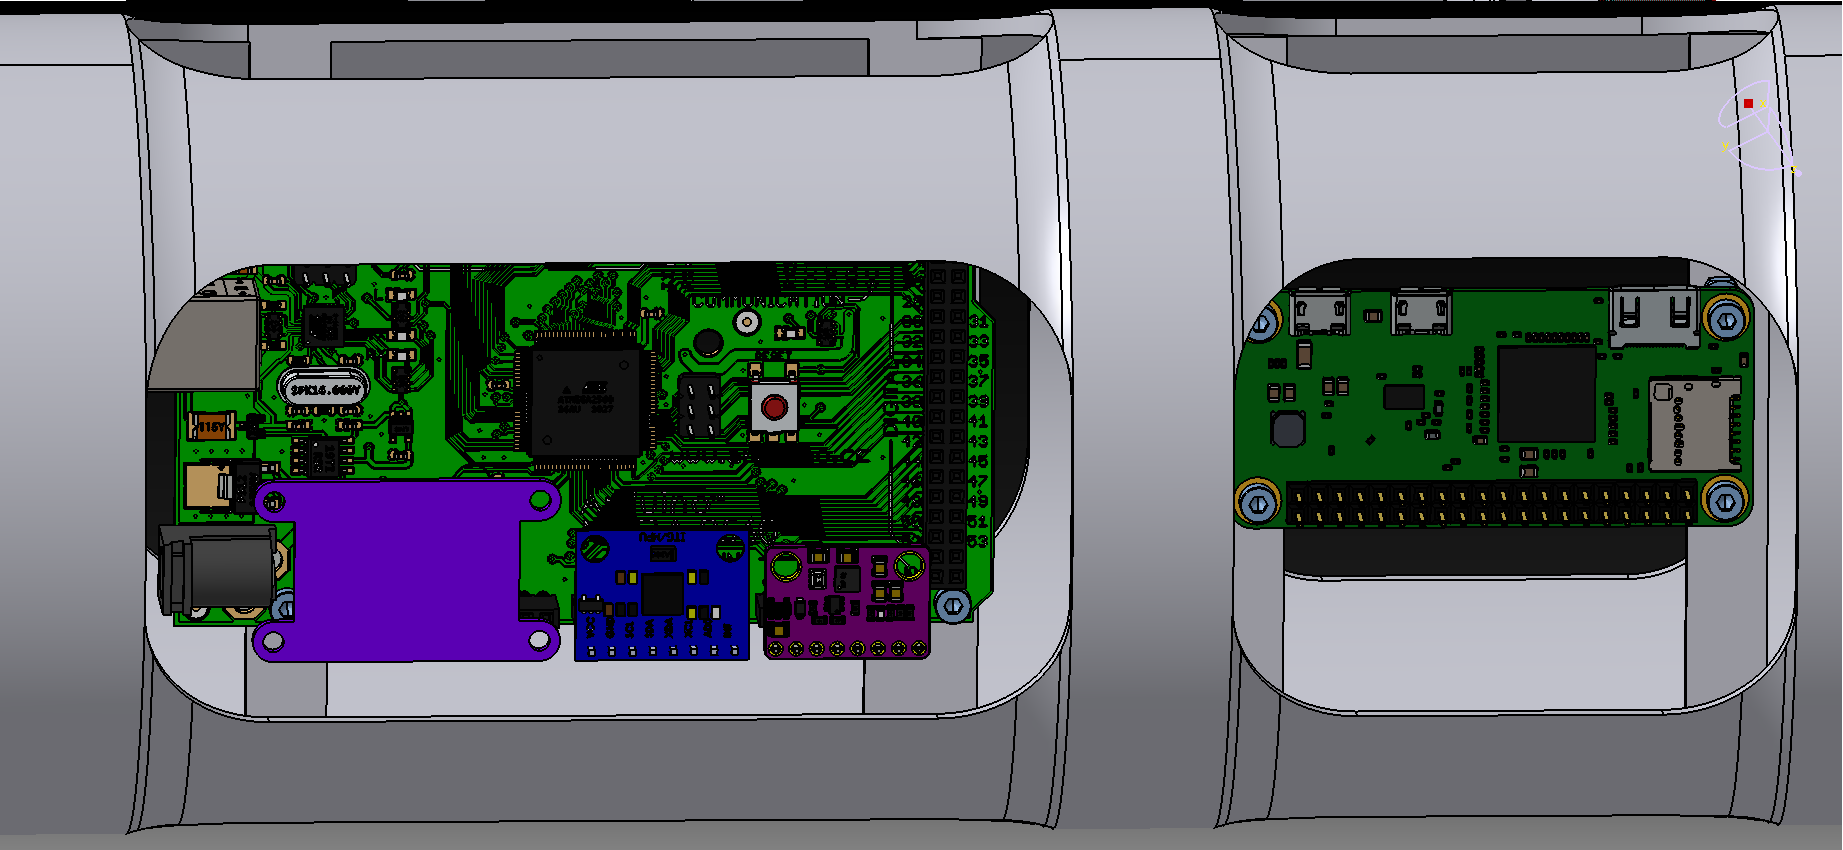
\includegraphics[height=0.2\pdfpageheight]{fig/design/v6_4}
    \caption{Prototipo final, detalle aviónica.}
    \label{fig:design/v6_4}
\end{figure}


\begin{figure}[htb]
    \centering
    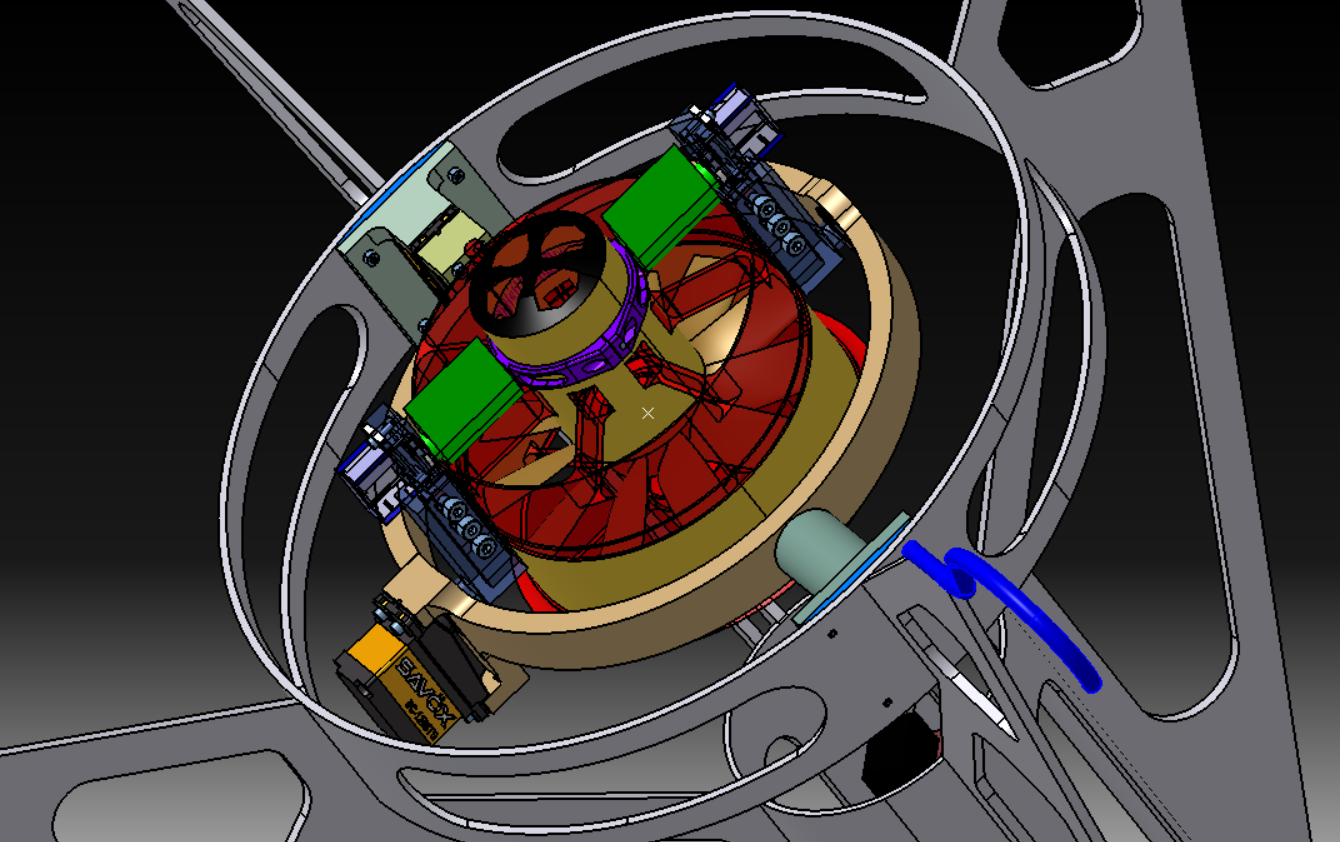
\includegraphics[height=0.25\pdfpageheight]{fig/design/v6_6}
    \caption{Prototipo final detalle de componentes.}
    \label{fig:design/v6_6}
\end{figure}

\begin{figure}[htb]
    \centering
    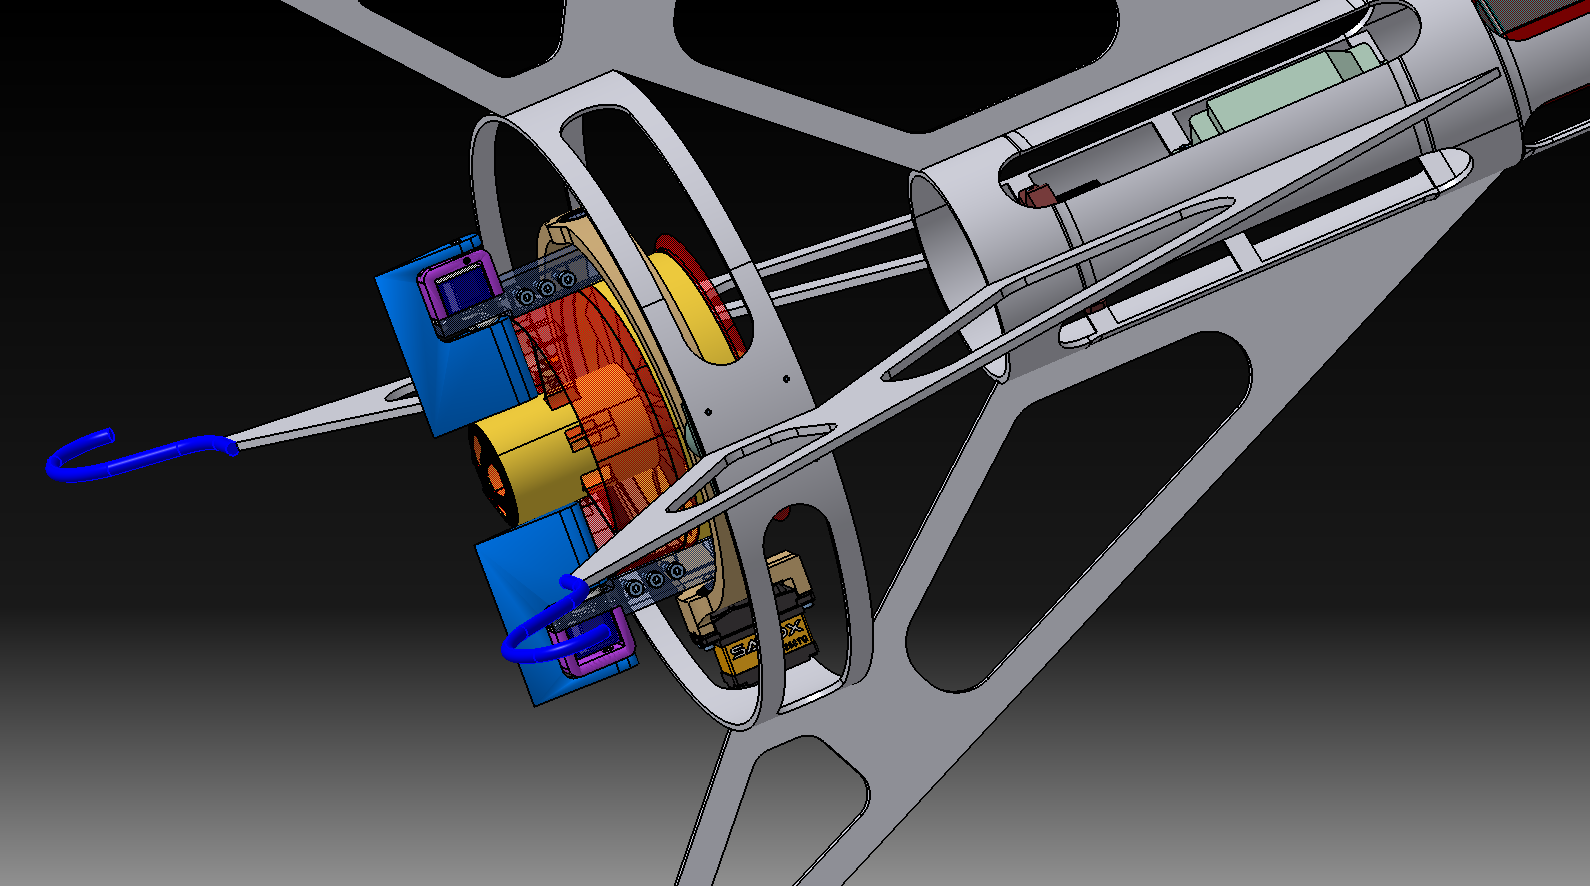
\includegraphics[width=\linewidth]{fig/design/v6_3}
    \caption{Prototipo final detalle EDF.}
    \label{fig:design/v6_3}
\end{figure}

\begin{figure}[htb]
    \centering
    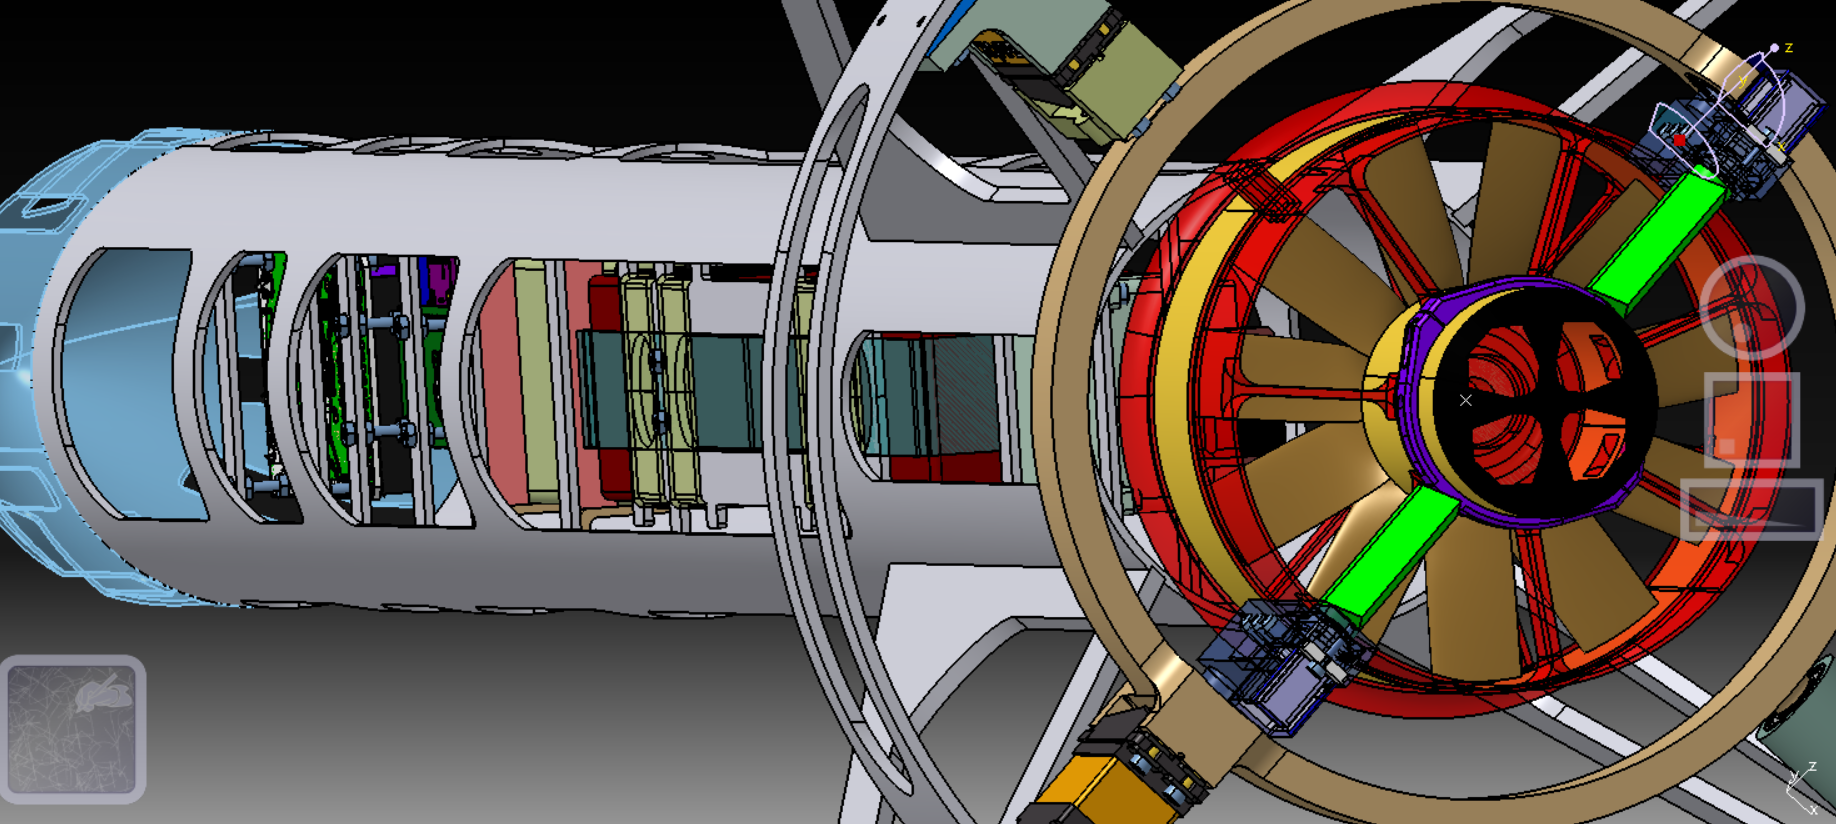
\includegraphics[width=\linewidth]{fig/design/v6_5}
    \caption{Prototipo final vista inferior detalle constructivo.}
    \label{fig:design/v6_5}
\end{figure}

\null\newpage
\clearpage

\subsection{Ensamblaje final - Fotos}
\begin{figure}[htb]
    \centering
    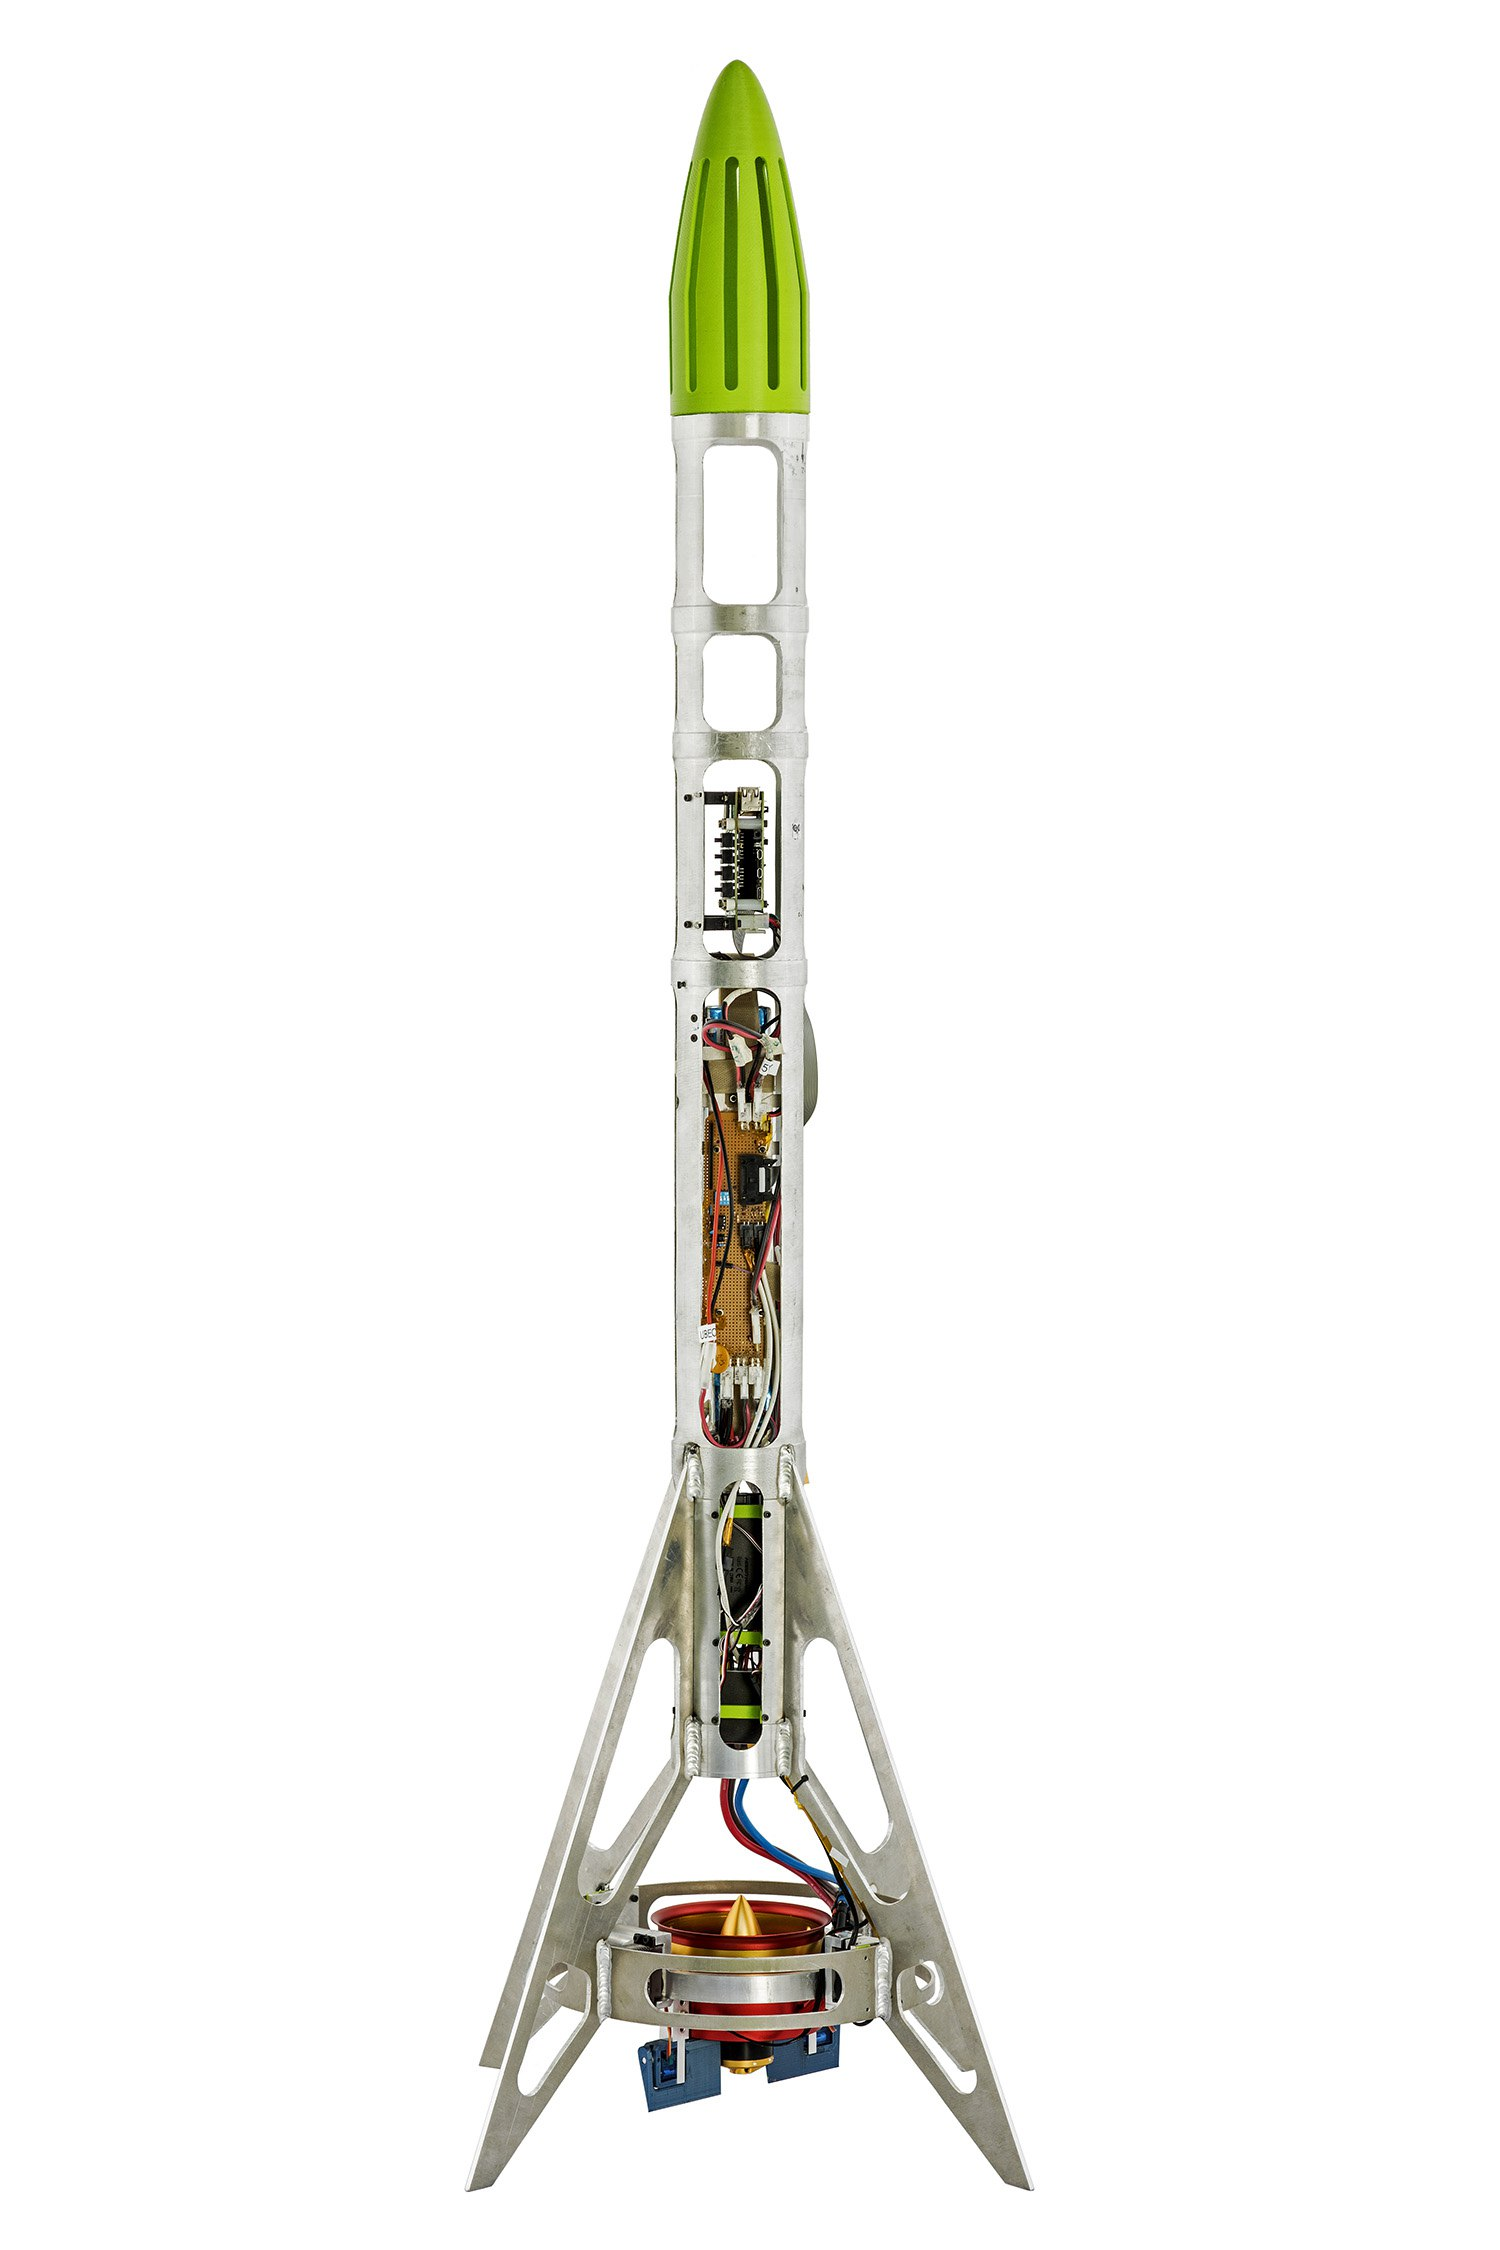
\includegraphics[height=0.6\pdfpageheight]{fig/hq/wide_plane_bonete.jpg}
    \caption{Foto del conjunto armado.}
    \label{fig:hq/wide_plane_bonete}
\end{figure}

\begin{figure}[htb]
    \centering
    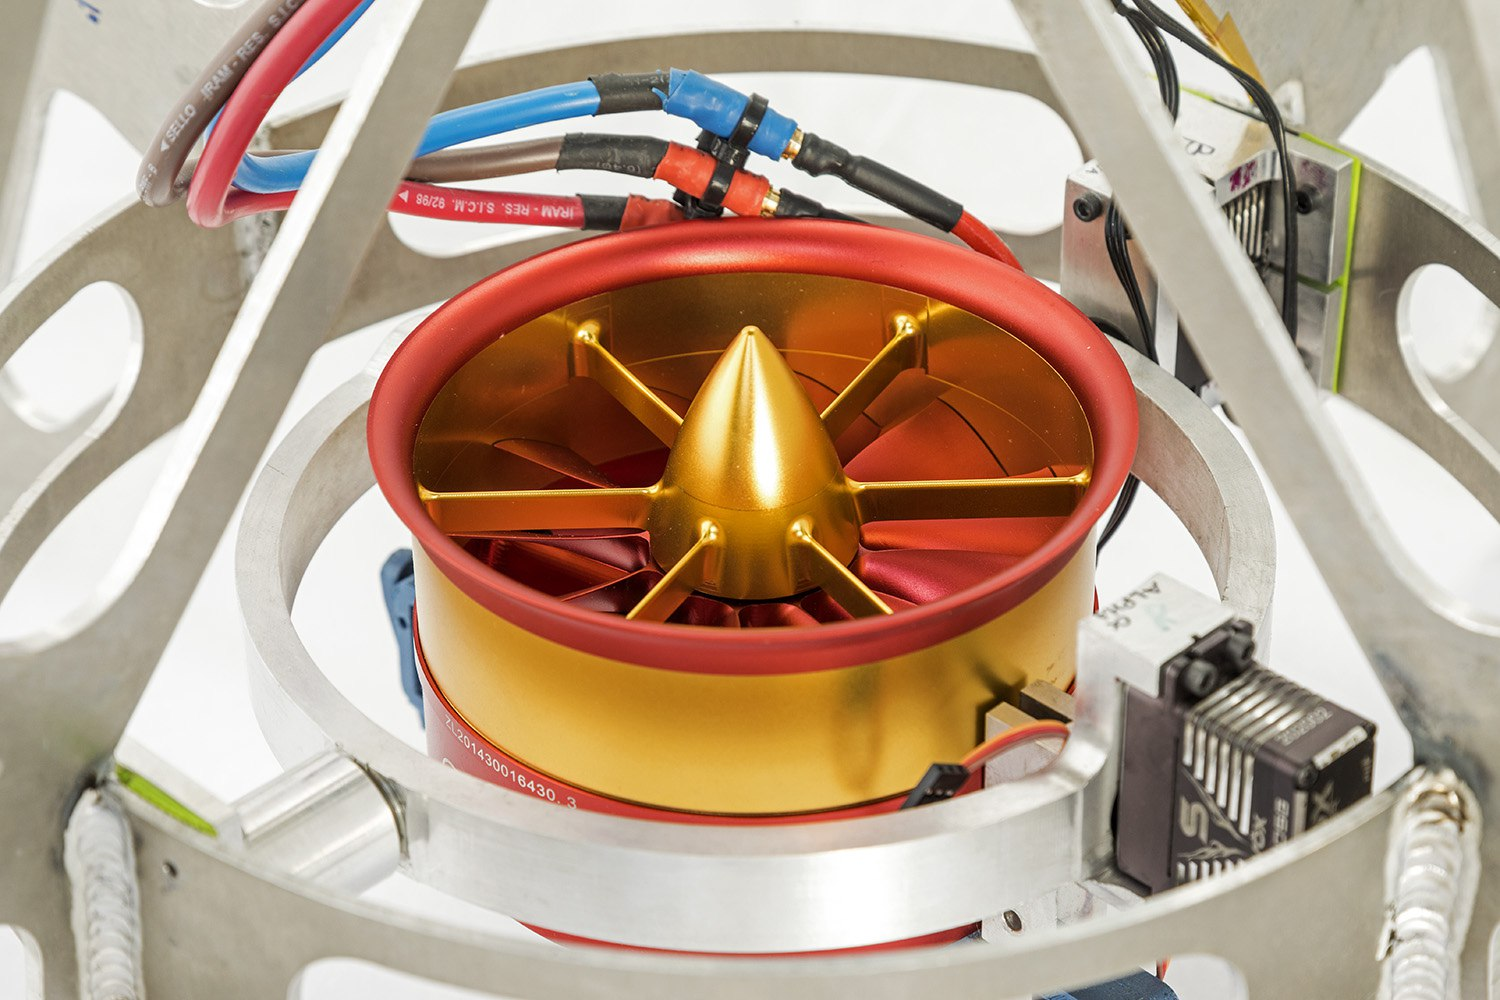
\includegraphics[height=0.3\pdfpageheight]{fig/hq/gimbal_close.jpg}
    \caption{Conjunto cardán, servos y soportes de gimbal externo.}
    \label{fig:hq/gimbal_close}
\end{figure}

\begin{figure}[htb]
    \centering
    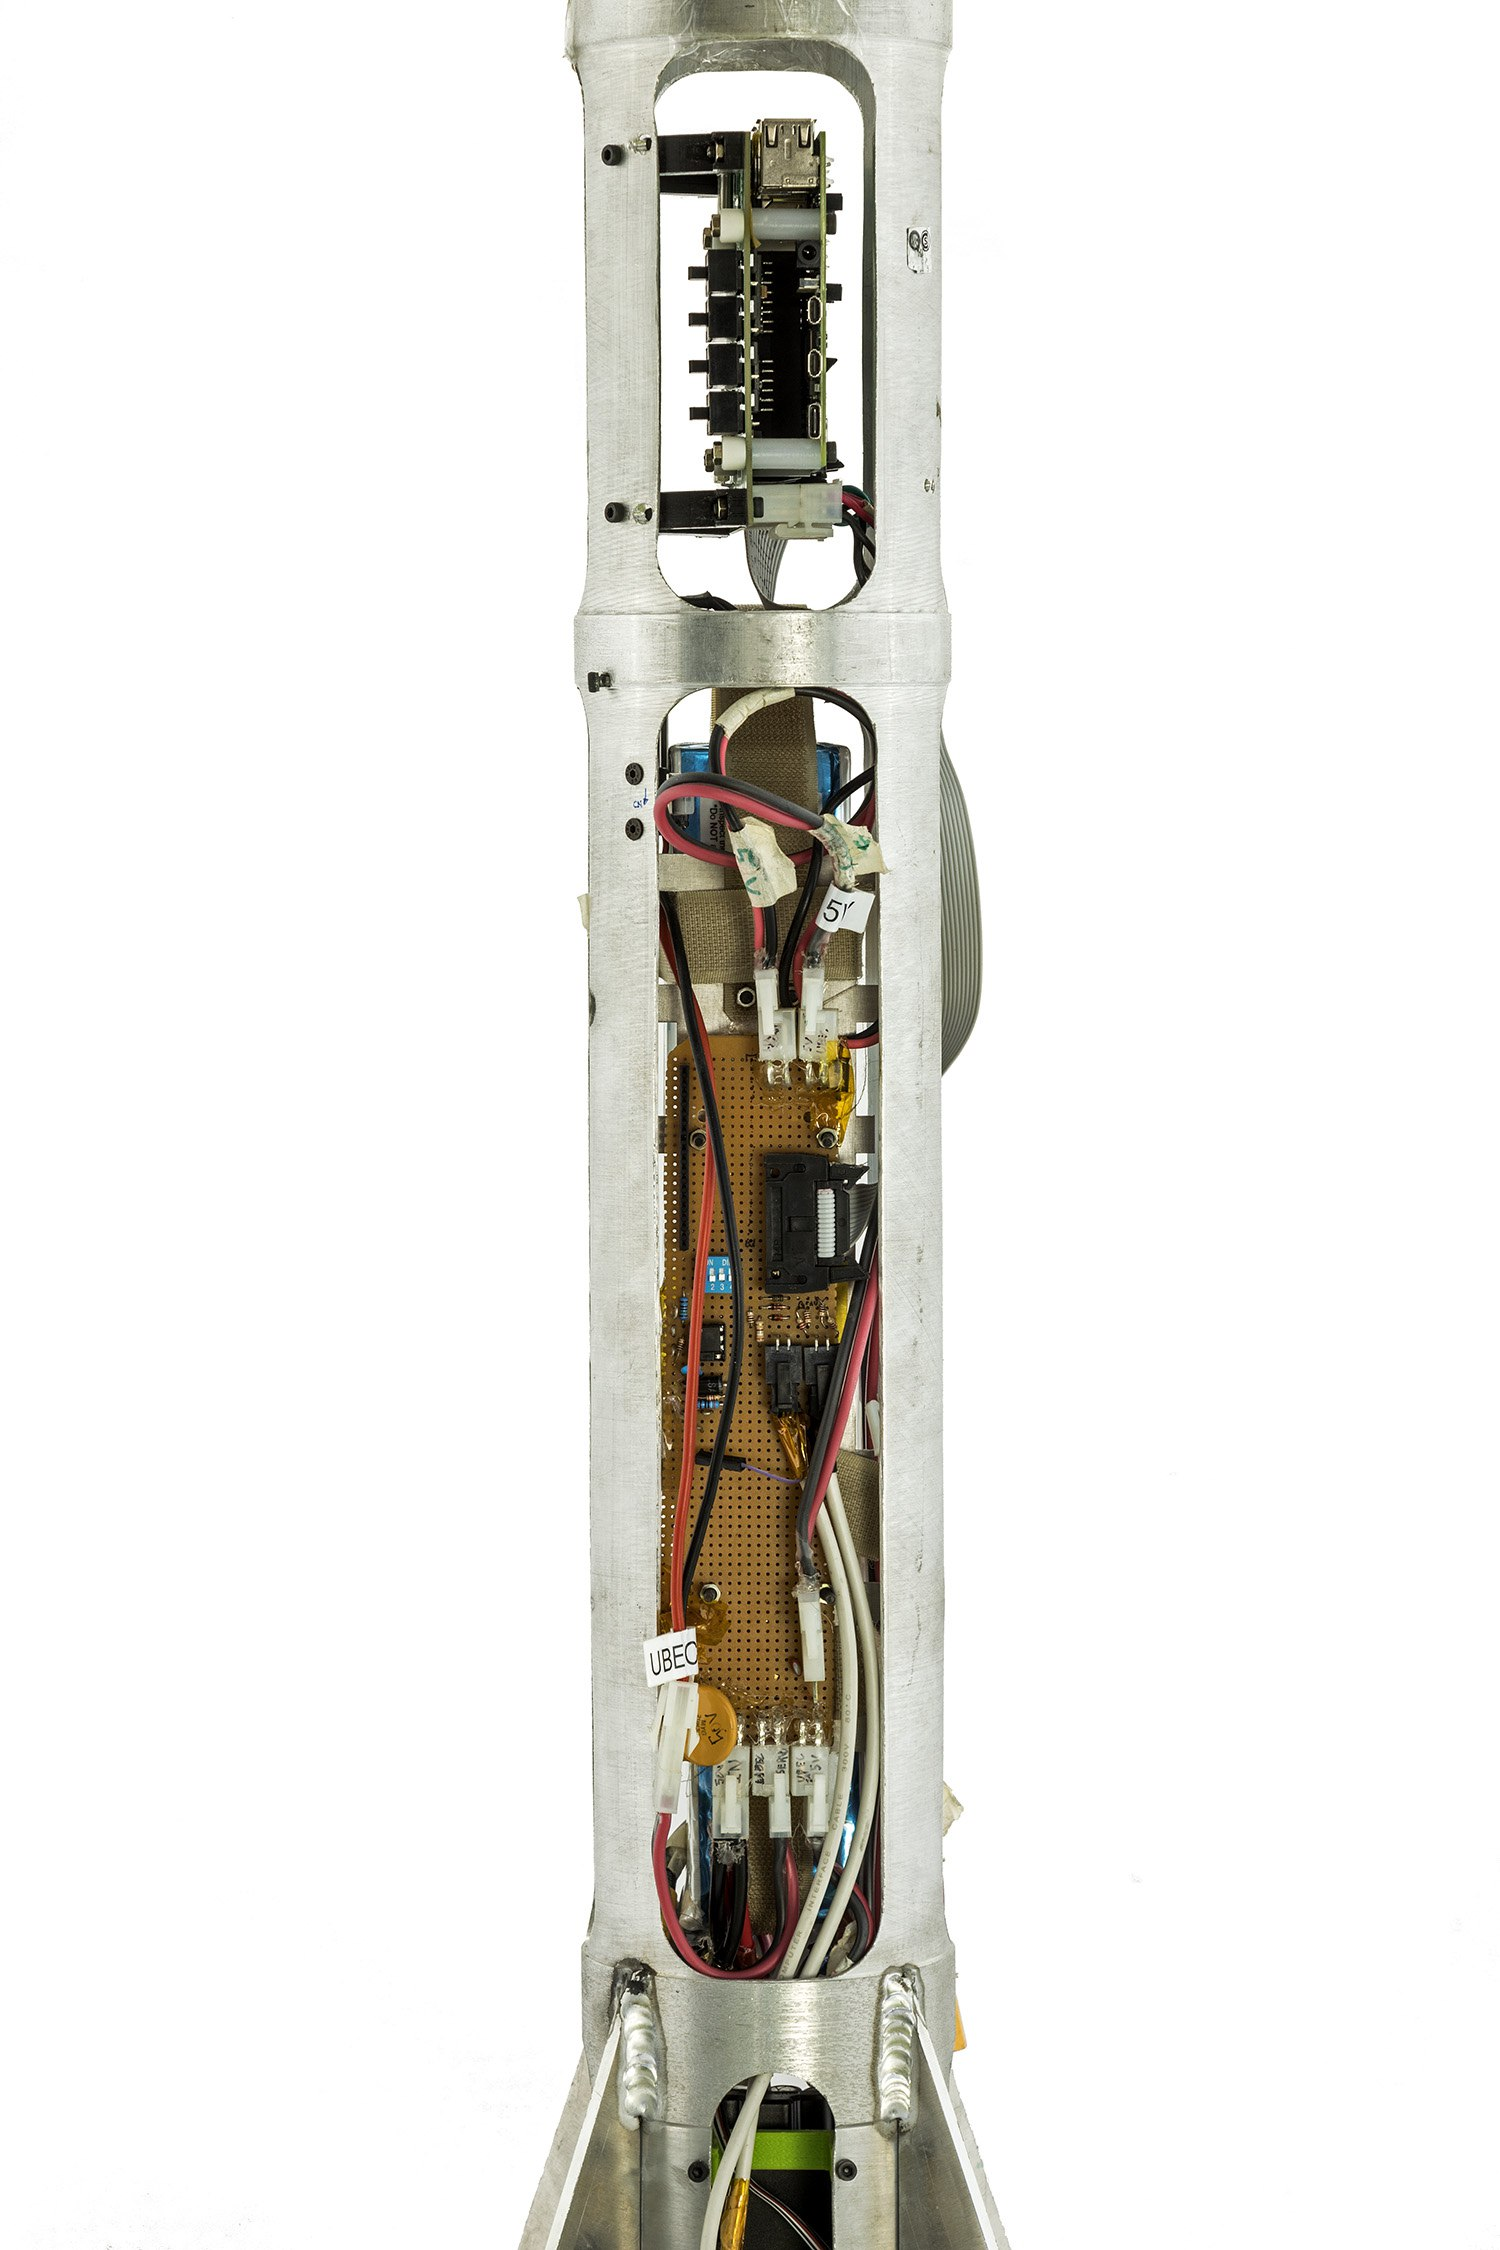
\includegraphics[height=0.3\pdfpageheight]{fig/hq/electronics.jpg}
    \caption{Conjuntos electrónica y cableado.}
    \label{fig:hq/electronics}
\end{figure}

\begin{figure}[htb]
    \centering
    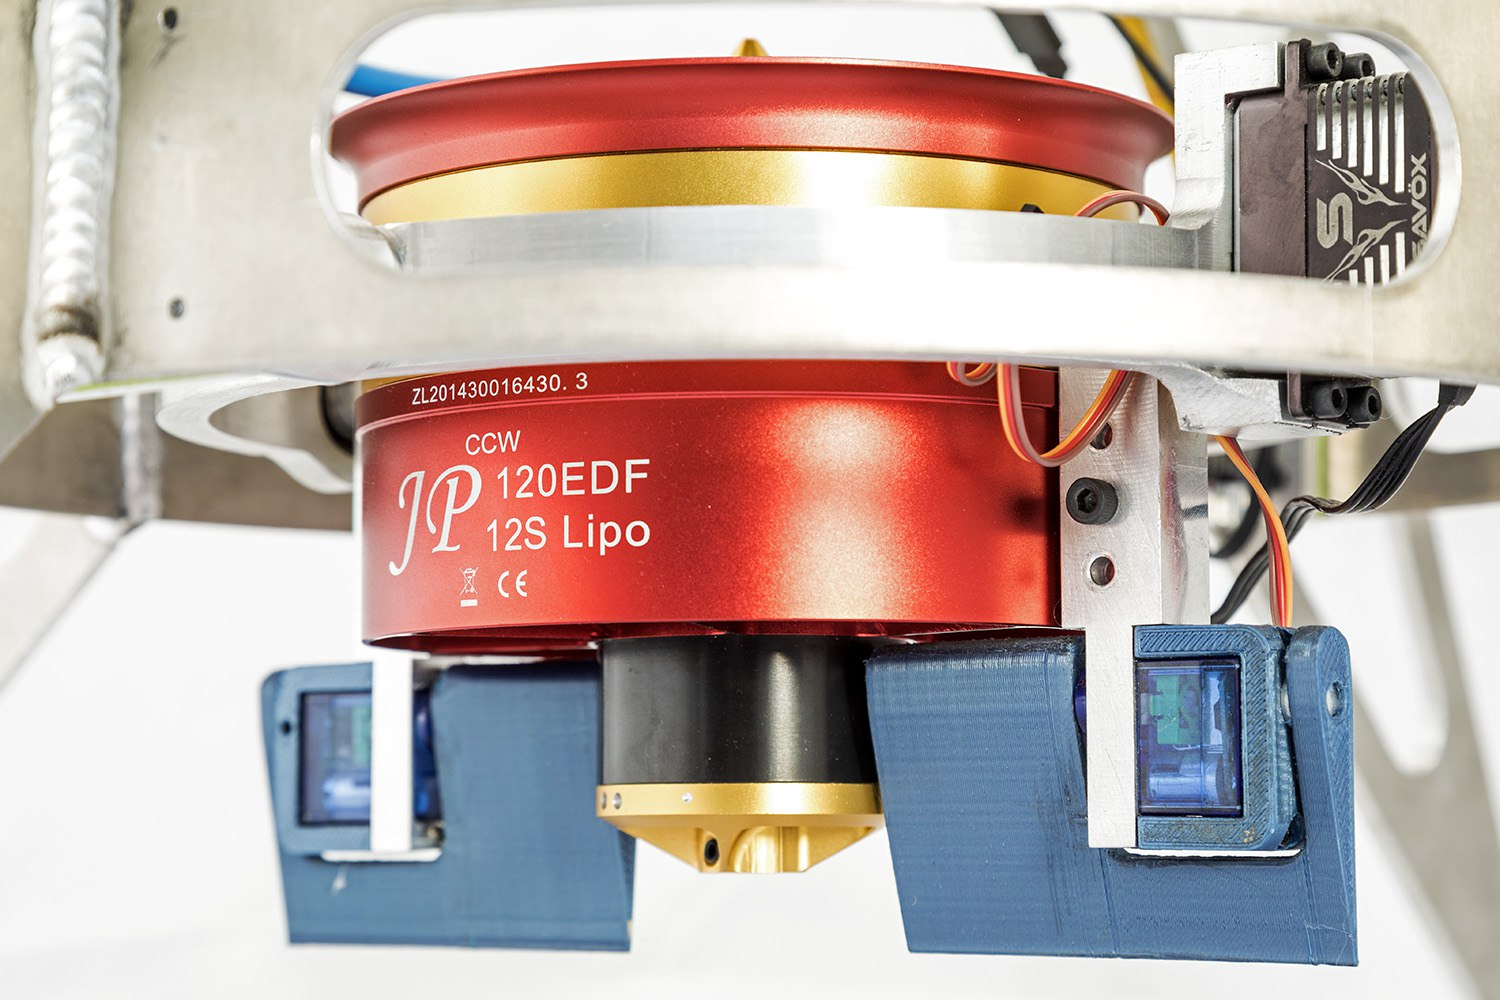
\includegraphics[height=0.3\pdfpageheight]{fig/hq/flaps.jpg}
    \caption{Vista inferior del conjunto cardán y flaps.}
    \label{fig:hq/flaps}
\end{figure}

\begin{figure}[htb]
    \centering
    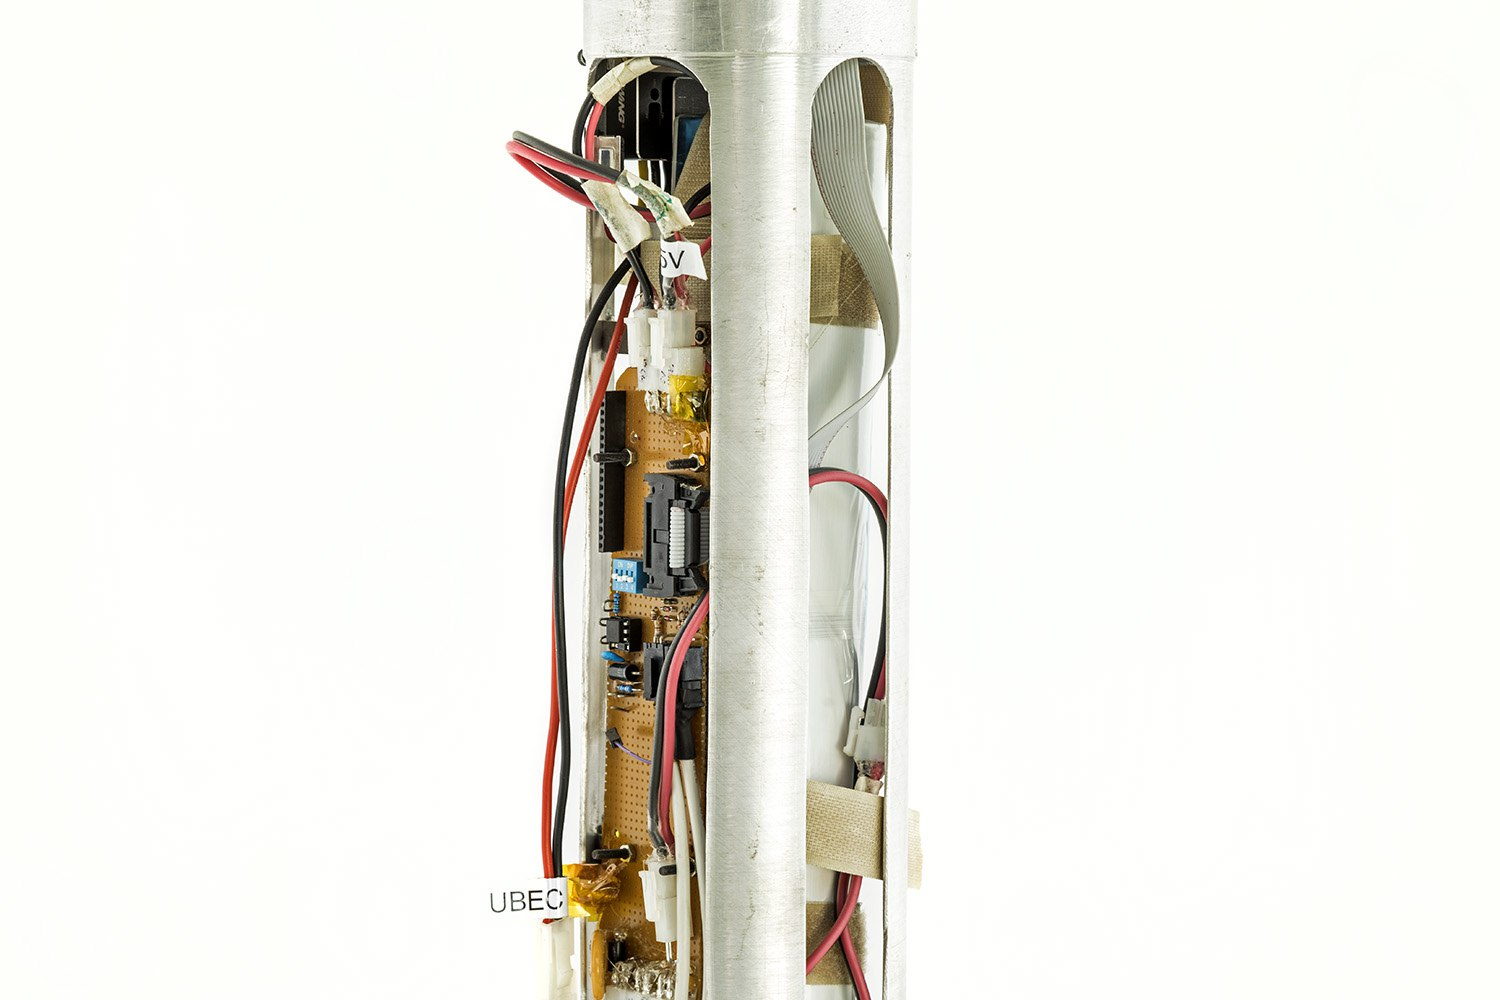
\includegraphics[height=0.3\pdfpageheight]{fig/hq/backpcb.jpg}
    \caption{Plano detalle de la placa electrónica de potencia.}
    \label{fig:hq/backpcb}
\end{figure}



\null\newpage
\clearpage


\section{Modelo 2D simplificado} \label{sec:model2d}

Esta siguiente sección detallará el tratamiento matemático efectuado para controlar un vehículo con propulsión vectorizada en el plano. El propósito es ilustrar a un nivel simple las herramientas que se aplicaron para controlar el vehículo diseñado.

\begin{figure}[htb!]
	\centering
	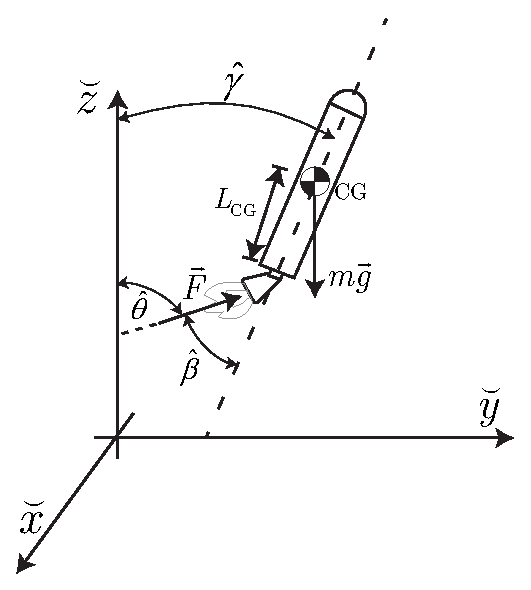
\includegraphics[width=9cm]{fig/rocketFBD.eps}
	\caption{Diagrama de cuerpo libre de un vehículo con propulsión vectorizada 2D.}
	\label{fig:FBD2D}
\end{figure}


\subsection{Modelado matemático}
Se comenzó con las ecuaciones dinámicas de un vehículo en el plano con control de propulsión vectorizada (por ángulo)

\[
\left\{
\begin{array}{l}
	\ddot{y}=\frac{F}{m} \sin(\gamma+\beta) \\
	\ddot{z}=\frac{F}{m} \cos (\gamma+\beta)-g \\
	\ddot{\gamma} = \frac{L_{\CG}\cdot F}{I_{xx}}\sin\beta
\end{array}
\right.
\]
donde \(\LCG\) y \(F\) están en función del tiempo, $m =m_0 - \int \dot{m} $ y $\theta = \gamma+\beta$. 

Vale la pena aclarar que no se tomaron en cuenta los siguientes efectos:
\begin{itemize}
	\item Viento y efectos aerodinámicos
	\item \textit{Fuel sloshing}
	\item Efectos relativistas
\end{itemize}

\subsection{Armado de sistema lineal}

Se propuso un punto de operación alrededor del cual se efectuó la linealización de las ecuaciones. El estado del vehículo alrededor del cual se linealizó fue \textit{vertical y quieto en el espacio}.\footnote{La linealización es valida solo para un vehículo vertical. Se deberá modificar el método para modelar un vehículo orbital.} 

\begin{align*}
	\gamma^* = 0 \\
	\beta^* = 0 \\
	F^* = mg
\end{align*}
en este caso $F$ fue la desviación del punto de operación siendo $\Delta F = F- mg$.

\subsection{Representación en espacio de estados}
El número de variables de estado fue igual a número de almacenadores de energía independientes. Estos son

\begin{enumerate}
	\item[$z$] Energía potencial por la gravedad
	\item[$\dot{y},\dot{z}$] Energía cinética del vehículo
	\item[$\dot{\gamma}$] Momento angular del vehículo
\end{enumerate}
entonces, las variables de estado fueron las siguientes
\begin{align*}
	x_1 = y \\
	x_2 = \dot{y} \\
	x_3 = z \\
	x_4 = \dot{z} \\
	x_5 = \gamma \\
	x_6 = \dot{\gamma}
\end{align*}
donde $\dot{x_1} = x_2$, $\dot{x_3} = x_4$ y $\dot{x_5} = x_6$

Se aprovecho la expansión de Taylor para la linealización de expresiones trigonométricas:
\[
\sin(x+y)|_{x=x_0+\Delta x,y=y_0+\Delta y} \approx \sin(x_0+y_0) + \cos(x_0 + y_0) (x-x_0) + \cos(x_0 + y_0) (y-y_0)
\]
\todo{Revertir cambios tiempo pasado}
Las ecuaciones dinámicas de los estados 2,3, y 4 fueron dadas por las ecuaciones mostradas al comienzo de esta sección.

Abajo se encuentran las ecuaciones de estados
\begin{equation}
	\dot{x_2} = \frac{F}{m} \left( \gamma+\beta \right) = g x_5 + g u_2 
\end{equation}
\begin{equation}
\dot{x_4} = \frac{F}{m} - g =\frac{F-F_0}{m}= \frac{u_1}{m}
\end{equation}
\begin{equation}
\dot{x_6} = \frac{\LCG \cdot F}{I_{xx}} \beta = \frac{\LCG \cdot mg}{I_{xx}} u_2 
\end{equation}

donde $\Ts$ es el periodo de muestreo.

Los vectores de entrada y salida resultaron
\[
\Cme{u}(t) = \begin{bmatrix}
u_1 \\
u_2
\end{bmatrix} = \begin{bmatrix}
\Delta F \\
\beta
\end{bmatrix}
\]
\[
\Cme{y}(t) = \begin{bmatrix}
y_1 \\
y_2 \\
y_3
\end{bmatrix} = \begin{bmatrix}
y \\
z \\
\gamma
\end{bmatrix}
\]
tal que las ecuaciones de salida son

\begin{equation}
	y_1 = x_1 
\end{equation}
\begin{equation}
	y_2 = x_3
\end{equation}
\begin{equation}
	y_3 = x_5
\end{equation}

Se calcularon las matrices del sistema y de control ($\Mme{D} = [0]$)
\begin{equation} \label{eq:ssmatrices}
	\Mme{A} = 
	\left[\begin{array}{cccccc} 0 & 1 & 0 & 0 & 0 & 0\\ 0 & 0 & 0 & 0 & g & 0\\ 0 & 0 & 0 & 1 & 0 & 0\\ 0 & 0 & 0 & 0 & 0 & 0\\ 0 & 0 & 0 & 0 & 0 & 1\\ 0 & 0 & 0 & 0 & 0 & 0 \end{array}\right],\quad \Mme{B} = 
	\left[\begin{array}{cc} 0 & 0\\ 0 & g\\ 0 & 0\\ \frac{1}{m} & 0\\ 0 & 0\\ 0 & \frac{\LCG \cdot mg}{I_{xx}} \end{array}\right], \quad \Mme{C} =  \left[\begin{array}{cccccc} 1 & 0 & 0 & 0 & 0 & 0\\ 0 & 0 & 1 & 0 & 0 & 0\\ 0 & 0 & 0 & 0 & 1 & 0 \end{array}\right]
\end{equation}
El sistema mostrado en \eqref{eq:ssmatrices} es \textit{fully state controllable}.

\section{Ecuaciones de movimiento de cuerpo rígido} \label{sec:ecuacionesRigid}
A continuación se mostrarán las ecuaciones de movimiento en el espacio usadas para controlar el vehículo.
Se hará referencia a la figura \ref{fig:FBD2D} para explicar las variables en juego en el modelo 3D debido a la dificultad inherente de mostrar las 16 variables de estado en un dibujo del modelo 3D.

\begin{figure}[htb!]
	\centering
	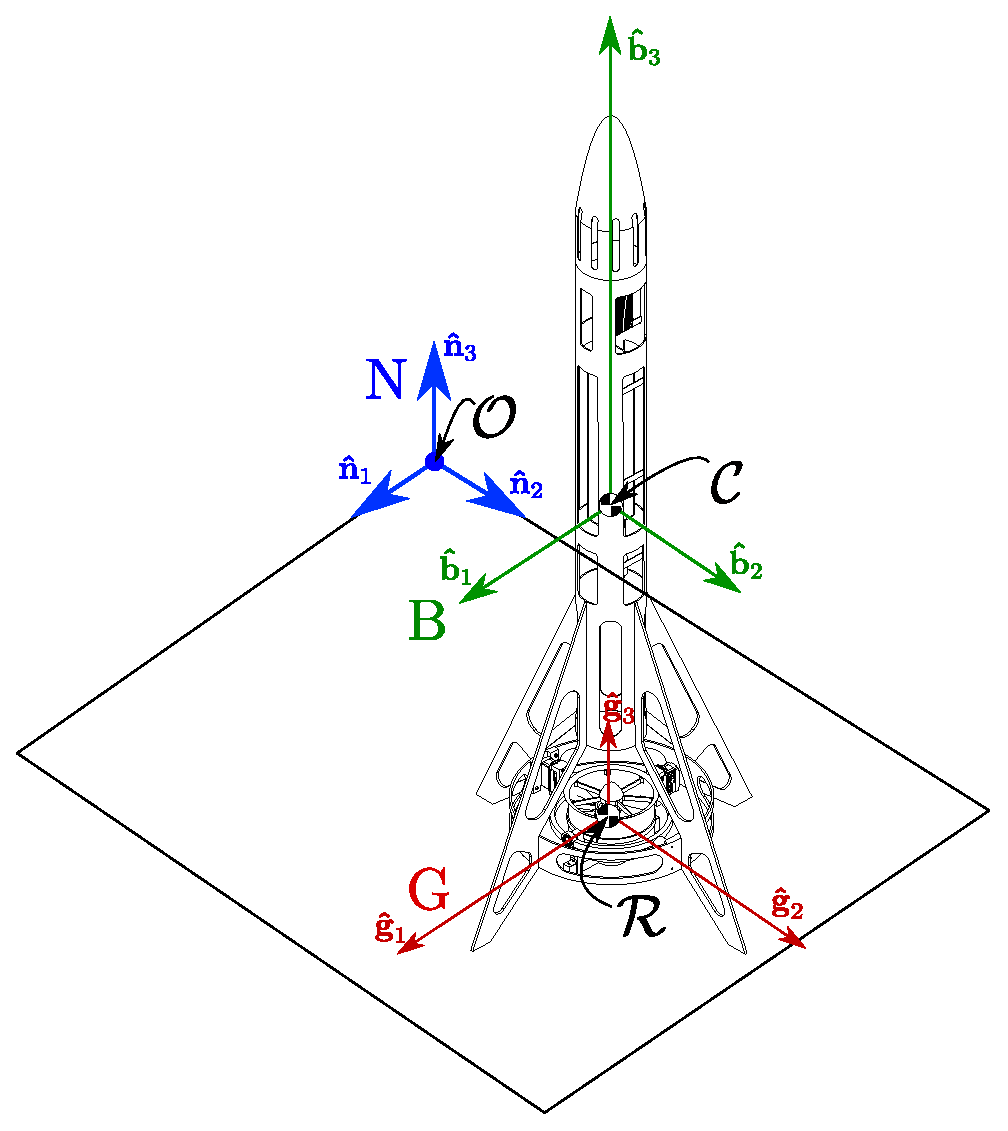
\includegraphics[width=0.52\textwidth]{fig/marcosDiagrama.eps}
	\caption{Marcos de referencia tomados para el análisis de cuerpo rígido. Por simplicidad se tomaron los centros de masa del cardán y del rotor como coincidentes en el punto $\ogn{R}$.}
\end{figure}

\newpage
\subsection{Notación}

La notación utilizada fue la del libro \textit{Rigid Body Dynamics of Mechanisms, Theoretical Basics} \cite{hahn2013rigid}. Se requirió un tratamiento algebraico explicito de los marcos de referencia y representación debido al caso especial de un \textit{gimballed rotor}. Este tratamiento facilitó la programación de la simulación y, en consecuencia, el control, el cual se volvería ambiguo y complejo con un tratamiento más común o simplificado.

\begin{description}
	\item[{\(\avec{r}_{\ogn{CO}}=[x,y,z]\)}] : Posición absoluta del centro de masa del vehículo léase ``posición de $\ogn{C}$ respecto $\ogn{O}$'')
	\item[{\(\avec{r}_{\ogn{RC}}\)}] : Posición del centro de masa del cardán respecto al centro de masa del vehículo
	\item[{\( \avec{\eta}=[\phi,\theta,\psi] \)}] : Ángulos de actitud del vehículo (Ángulos Euler)
	\item[\( \avec{\omega}_r^{\frm{G}} \)] : Velocidad angular del rotor del EDF representado en el marco $\frm{G}$ (dirección constante)
	\item[\( \avec{\omega}_\frm{BN}^\frm{B} \)] : Velocidad angular de $\frm{B}$ respecto a $\frm{N}$, representado en el marco $\frm{B}$.
	\item[\(  \alpha, \beta \)] : Ángulo de actuación de vectorización del EDF o ángulo de actitud del marco $\frm{G}$
	\item[{\( \delta   \)}] :  Ángulo de actuación de los dos flaps anti-roll
	\item[{\( m  \)}] :  Masa del vehículo sin rotor
	\item[{\( m_r  \)}] :  Masa del rotor
	\item[{\( \avec{g}  \)}] :  Aceleración de la gravedad
	\item[{\( \avec{F}^\frm{B} \)}] : Empuje del EDF representado en el marco $\frm{B}$ 
	\item[{\( \transform{NB}  \)}] :  Matriz de transformación de cosenos directores de un marco $\frm{B}$ a el marco $\frm{N}$
\end{description}

\textbf{Caracterización del EDF}
\begin{description}
	\item[{\( \tau_c  \)}] :  Torque efectivo de control del EDF
%	\item[{\( i  \)}] :  Corriente entregada al motor
	\item[{\( K_T  \)}] :  Constante de empuje del EDF
	\item[{\( K_Q  \)}] :  Coeficiente de torque viscoso de fricción
	\item[{\( Q  \)}] :  Torque viscoso de fricción
	\item[{\( \tau_r \)}] : Torque de reacción por el swirl de salida
\end{description}

\textbf{Caracterización del mecanismo anti-roll:}
\begin{description}
	\item[{\( K_{F_L}  \)}] : Coeficiente de lift de los flaps anti-roll
	\item[{\( K_{F_D}  \)}] : Coeficiente de drag de los flaps anti-roll
	\item[{\( F_L \)}] : Lift de los flaps anti-roll
	\item[{\( F_D \)}] : Drag de los flaps anti-roll
\end{description}

\textbf{Matriz de inercia:}
\begin{description}
	\item[{\(  \inertia{C}{B}  \)}] : Vehículo sin rotor respecto a $\ogn{C}$ representado en $\frm{B}$
	\item[{\(  \inertiarotor{R}{G}  \)}] : Rotor respecto a $\ogn{R}$ representado en $\frm{G}$
	\item[{\(  \inertia{\!\mathrm{g}R}{G}  \)}] : Cardán y motor sin rotor respecto a $\ogn{R}$ representado en $\frm{G}$
\end{description}



\subsection{Notación del álgebra a utilizar}

El producto escalar se definió como $\bigcdot$ para diferenciarlo de simple multiplicación vectorial ($\cdot$). $\skw{\omega}$ es la matriz skew del vector que reemplaza el producto vectorial ya que $\skw{r}\cdot v = r \times v$
\[
\skw{\omega}_{L R}^{L}=\left(\begin{array}{ccc}
0 & -\omega_{z L R}^{L}, & \omega_{y L R}^{L} \\
\omega_{z L R}^{L} & 0 &-\omega_{x L R}^{L} \\
-\omega_{y L R}^{L} &  \omega_{x L R}^{L} & 0
\end{array}\right)
\]

Se definió a $J_\ogn{C}^\frm{B}$ como la matriz de inercia respecto al punto $\ogn{C}$, representada en el marco $\frm{B}$: es decir, las componentes de la matriz de inercia están en la base de $\frm{B}$. Esto se puede escribir así:
\begin{IEEEeqnarray*}{c}
J_\ogn{C}^\frm{B} = J_{b1} \bvec{b}_1 + J_{b2} \bvec{b}_2 + J_{b3} \bvec{b}_3
\end{IEEEeqnarray*}

La derivada del término anterior respecto un marco $N$ quedó definida
$${}^\frm{N}\dot{J}_{\ogn{C}}^\frm{B} =\left.^\frm{N} \frac{\di J_\ogn{C}^\frm{B}}{\di t}  \right. = \transform{NB} \cdot \left.^\frm{B} \frac{\di J_\ogn{C}^\frm{B}}{\di t}  \right. $$


Se pueden demostrar las siguientes ecuaciones
\begin{IEEEeqnarray}{C}
\dottransform{RL} =\transform{RL}\cdot \skw{\omega}^\frm{L}_\frm{LR} =
\skw{\omega}^\frm{R}_\frm{LR}\cdot\transform{LR} = -\skw{\omega}^\frm{L}_\frm{LR}\cdot\transform{RL} \\
\transform{BN} = (\transform{NB})\tp =  (\transform{NB})^{-1} \quad \Rightarrow \quad \transform{NB} \cdot \transform{BN} = \eye
\end{IEEEeqnarray}

donde $\omega_{\frm{LR}}^{\frm{L}}$ es la velocidad angular vectorial del marco $\frm{L}$ con respecto a $\frm{R}$ representado en $\frm{L}$, $\transform{RL}$ es la matriz de cosenos directores que transforma una vector de una base ortogonal $\frm{L}$ a otra base ortogonal $\frm{R}$, y $\dottransform{RL}$ es la derivada de la matriz $\transform{RL}$ respecto $\frm{R}$.

\newpage

\subsection{Variables de estado}
Se obtuvieron las variables de estado de posición y velocidad donde $z$ positivo es alejándose de la tierra.
\[
\avec{r}_\ogn{CO}^\frm{N} = 
\begin{bmatrix}
x & y & z 
\end{bmatrix}, \qquad
\dot{\avec{r}}_\ogn{CO}^\frm{N} = 
\begin{bmatrix}
\dot{x} & \dot{y} & \dot{z}
\end{bmatrix} 
\]

El movimiento cuerpo rígido se describió por 3 ángulos de Euler (Cardán o Bryant en algunas bibliografías) $\phi, \theta$ y $\psi$ (roll, pitch, yaw respectivamente).
\begin{IEEEeqnarray}{C}
\avec{\eta} = \begin{bmatrix}
\phi  &  \theta &  \psi
\end{bmatrix}
\end{IEEEeqnarray}

\begin{figure}[ht!]
	\centering
	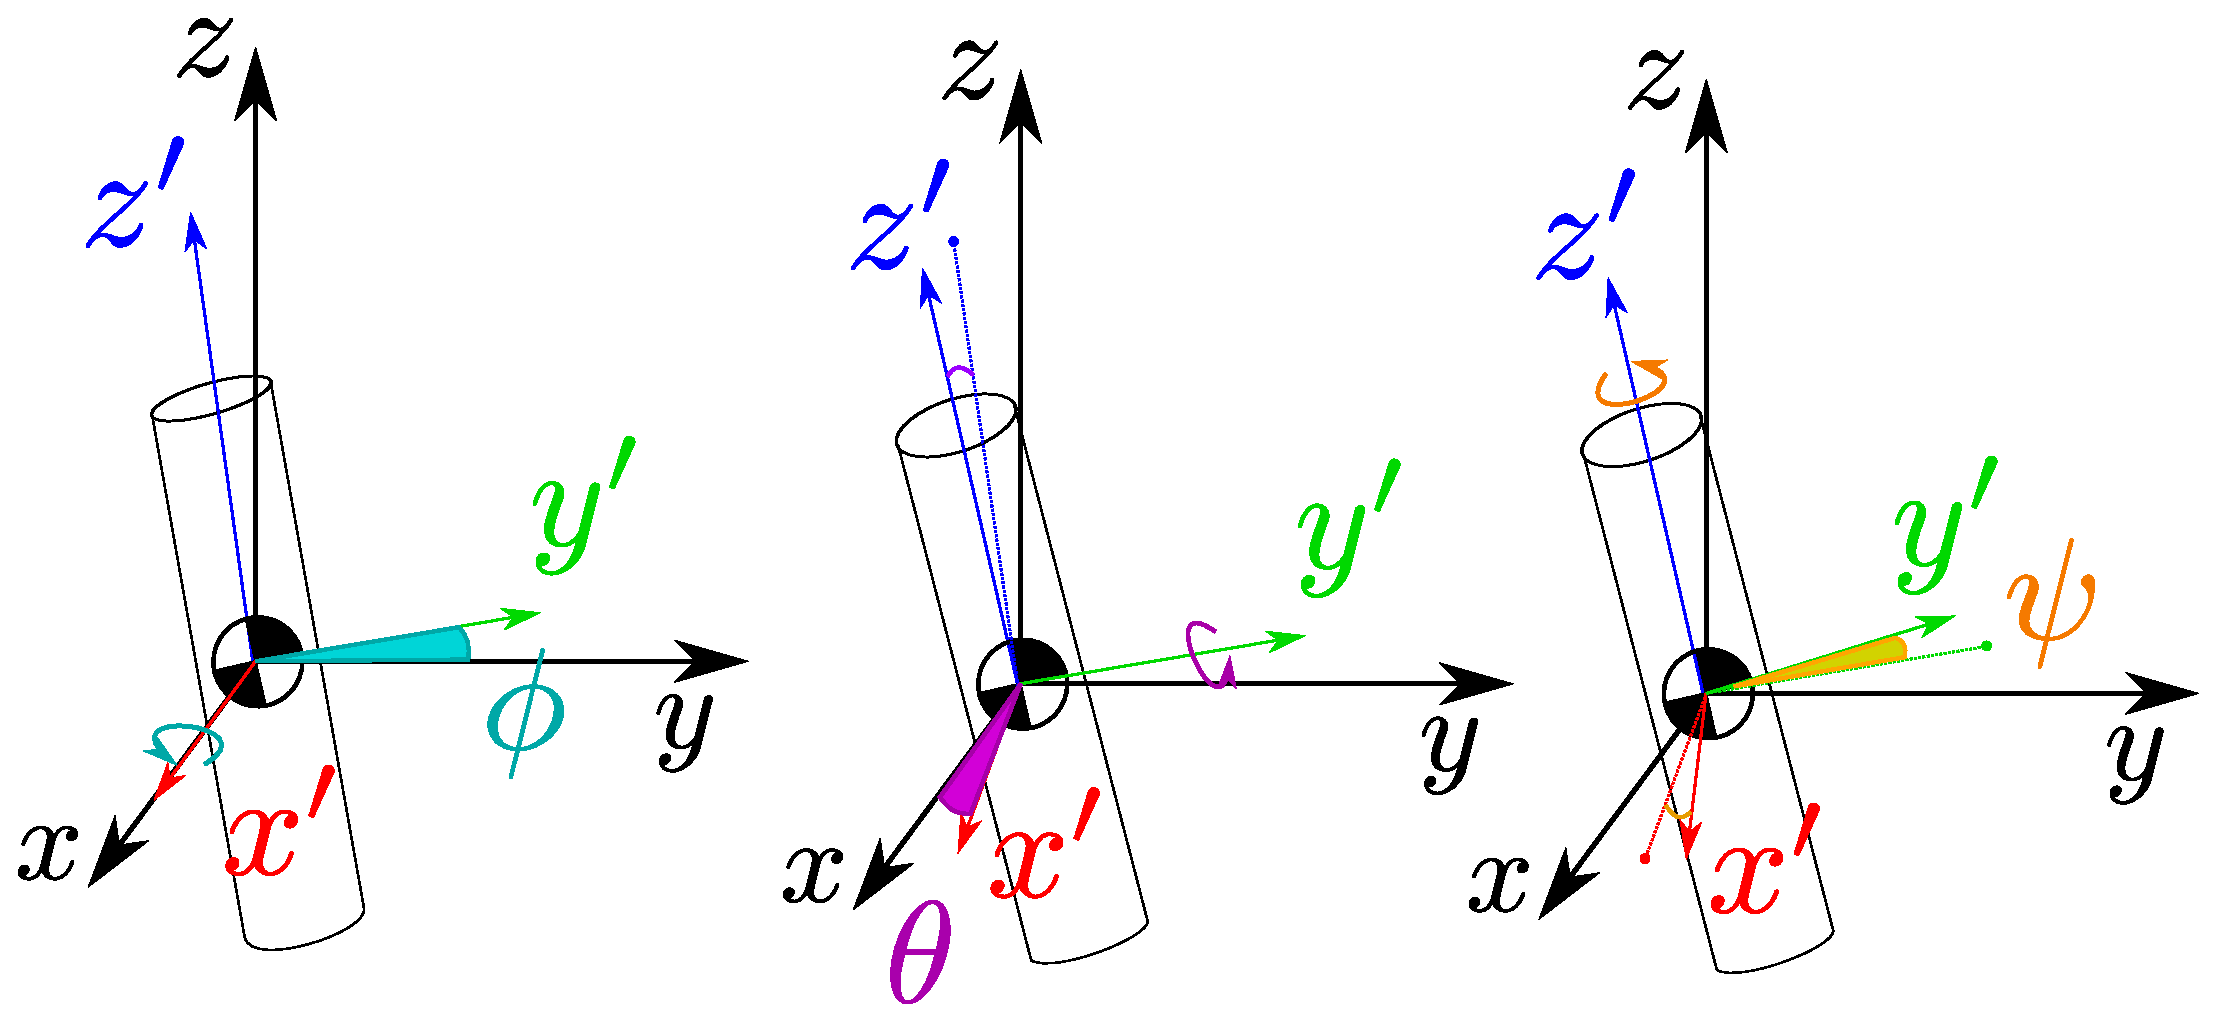
\includegraphics[width=0.8\textwidth]{fig/cuerpolibreGlobal_v2.eps}
	\caption{Diagrama mostrando las rotaciones de ángulo de euler en el orden que son efectuadas para describir el sistema. $\phi$ representa el pitch, $\theta$ el yaw y $\psi$ el roll. Se muestran las últimas posiciones de los ejes rotados con una linea punteada.}
\end{figure}


Los ángulos de la vectorización de la tobera fueron $\alpha$ y $\beta$. El ángulo $\delta$ correspondió a los actuadores que contrarrestan el roll del vehículo mediante dos flaps. Los ángulos $\alpha$ y $\beta$ describieron la dirección en la que está apuntando la tobera (equivalente a la orientación $\frm{G}$) respecto la dirección del vehículo (marco $\frm{B}$). $\omega_r=\omega_r^\frm{G}$ es la velocidad angular del rotor.

\medskip

Se definieron las variables de estado y el vector input, donde $F$ es la fuerza que hace la tobera sobre el vehículo (la cual depende de la velocidad del vehículo)\footnote{En el código $\phi$, $\theta$ y $\psi$ aparecen como \texttt{q,r,s}}
\begin{equation} \label{eq:ssVariables3D}
	\Cx = \left[
	\begin{array}{cccccccc}
		\avec{r}_\ogn{CO}^\frm{N} & \avec{\eta} &\dot{\avec{r}}_\ogn{CO}^\frm{N} &  \avec{\omega}_\frm{BN}^\frm{B} & \omega_r & \alpha & \beta & \delta
	\end{array}\right] \tp
\end{equation}
\begin{equation}\label{eq:ssInputs3D}
	\Cu = \begin{bmatrix}
		\tau_c & \dot{\alpha} & \dot{\beta} & \dot{\delta}
	\end{bmatrix} \tp
\end{equation}
En la próxima sección se buscará obtener el vector de variables de estado derivado en el tiempo $\dot{\Cx}$.

\subsection{Ecuaciones diferenciales} \label{subsec:modeloMatematico}

\def\scos{\operatorname{c}}
\def\ssin{\operatorname{s}}
Se definió la transformación de los ángulos euler con una matriz de transformación $\transform{BN}$ donde $\scos$ y $\ssin$ fueron las funciones coseno y seno, respectivamente.

\begin{equation} \label{eq:matrizTransfoVehiculo}
	\transform{BN} = \begin{bmatrix}
	\scos \theta \cdot \scos \psi & \scos \theta \cdot \ssin \psi & - \ssin \theta \\
	\ssin \phi \cdot \ssin \theta \cdot \scos \psi - \scos \phi \cdot \ssin \psi & \ssin\phi \cdot \ssin\theta \cdot \ssin\psi + \scos\phi\cdot\scos\psi & \ssin\phi \cdot \scos\theta \\
	\scos\phi \cdot \ssin\theta \cdot \scos\psi + \ssin\phi \cdot \ssin\psi\quad & \scos\phi \cdot \ssin\theta \cdot \ssin\psi - \ssin\phi \cdot \scos\psi \quad& \scos\phi \cdot \scos\theta
	\end{bmatrix}
\end{equation}
La transformación nos sirvió para poder pasar de la dinámica que está definida en el marco del vehículo $\frm{B}$ al marco $\frm{N}$ donde se obtienen las variables de estado que se desean controlar.

Se pudo obtener la velocidad en el marco del cuerpo
\begin{IEEEeqnarray}{rCl}
	\dot{\avec{r}}_\ogn{CO}^\frm{B} &= &\transform{BN} \cdot \dot{\avec{r}}_\ogn{CO}^\frm{N} 
\end{IEEEeqnarray}

La obtención de la velocidad angular del cuerpo se complicó por el hecho de que la razón de cambio de los ángulos de Euler no son vectores cartesianos, si no más bien parámetros que describen la orientación del cuerpo rígido en el espacio.\footnote{ Como bien sabemos la matriz de transformación $\tform$ solo es aplicable para transformar vectores cartesianos de una base ortogonal a otra. Los parámetros $\avec{\eta}$ conforman un vector de configuración, no un vector cartesiano!} Para relacionar la velocidad angular con $\avec{\eta}$ fue necesario utilizar la matriz de actitud cinemática $\attitude(\avec{\eta})$.

\begin{IEEEeqnarray}{c}
	\attitude(\avec{\eta}) = \left[\begin{array}{ccc}
	1 & \sin (\phi) \tan (\theta) & \cos (\phi) \tan (\theta) \\
	0 & \cos (\phi) & -\sin (\phi) \\
	0 & \sin (\phi) \sec (\theta) & \cos (\phi) \sec (\theta)
	\end{array}\right]
\end{IEEEeqnarray}

La matriz de actitud cinemática se usó para transformar 
\begin{IEEEeqnarray}{rCl}
	 \dot{\avec{\eta}}& = & \attitude(\avec{\eta}) \cdot  \avec{\omega}_\frm{BN}^\frm{N} \\
	\avec{\omega}_\frm{BN}^\frm{B} & = &\transform{BN}\cdot \avec{\omega}_\frm{BN}^\frm{N}
\end{IEEEeqnarray}
e inversamente
\begin{IEEEeqnarray}{rCl}
	\avec{\omega}_\frm{BN}^\frm{N} & = &\attitude^{-1}(\avec{\eta})\cdot \dot{\avec{\eta}} \\
\end{IEEEeqnarray}


La fuerza que impulsó al vehículo en el marco del cuerpo se obtuvo transformando del marco del cardán donde se conocen los componentes, al marco cuerpo. La matriz fue calculada reemplazando $\phi\equiv\alpha$, $\theta\equiv\beta$, y $\psi = 0$.
\begin{equation}
	\avec{F}^\frm{B} = \transform{BG} \cdot \avec{F}^\frm{G} 
\end{equation}

La aceleración del centro de masa del vehículo se midió en el marco del cuerpo $\frm{B}$ y fue igualada a  $\avec{F}$
\begin{equation}
	{}^\frm{B}\frac{\di }{\di t}\left( \dot{\avec{r}}_\ogn{CO}^\frm{B} \right) = \frac{1}{m+m_r} \cdot \avec{F}^\frm{B}
\end{equation}
luego obtenemos la aceleración en coordenadas globales
\begin{equation}
	\ddot{\avec{r}}_\ogn{CO}^\frm{N} =
	\transform{NB}\cdot {}^\frm{B}\frac{\di }{\di t}\left( \dot{\avec{r}}_\ogn{CO}^\frm{B} \right)- \avec{g}^\frm{N}
\end{equation}

Los momentos actuantes externos en el marco del vehículo respecto su centro de gravedad $\ogn{C}$ se calcularon en base al diseño de los flaps anti roll según~\cite{isaac2022mathematical}.
\todo{Se tiene que tratar el termino de la vorticidad aqui. Se puede suponer que la vorticidad forma parte del termino de flaps y que se modela como si fuera un offset del angulo de actuacion, es decir, cuando los flaps estan actuados en angulo cero va haber un momento debido a la vorticidad del flujo del EDF. Entonces a la ecuacion de abajo se le agrega un término constante al angulo del flap actuado para tomarlo en cuenta.}

\begin{equation}
	\avec{M}^\frm{B}_\ogn{C} = \skw{\avec{r}}_\ogn{RC}^\frm{B}\cdot \avec{F}^\frm{B} + \transform{BG} \cdot 
	\begin{bmatrix}
		0 \\
		0 \\
		\omega_r^2 K_{F_L}d_T\delta+\tau_r
	\end{bmatrix}  
\end{equation}

La aceleración angular en el marco $\frm{B}$ se obtuvó del desarrollo de la sección~\ref{ssec:ecuacionangular} del anexo.
\begin{equation}
	\hspace{-1cm}
{}^\frm{B}\frac{\di }{\di t} \left(\avec{\omega}_\frm{BN}^\frm{B} \right) =  \left(\inertia{C}{B}\right)^{-1} \cdot \left( - \skw{\avec{\omega}}_\frm{BN}^\frm{B} \cdot \inertia{C}{B}\cdot \avec{\omega}_{\frm{BN}}^{\frm{B}} - 
\transform{{BG}} \cdot\skw{\avec{\omega}}_\frm{GB}^\frm{G} \cdot \inertiarotor{R}{G}  \cdot \avec{\omega}_r^\frm{G} -
\skw{\avec{\omega}}_\frm{BN}^\frm{B} \cdot \inertiarotor{R}{G}  \cdot \avec{\omega}_r^\frm{G} -
\transform{{BG}}\cdot  \inertiarotor{C}{G} \cdot  {}^\frm{N} \dot{\avec{\omega}}_{\!r}^{\frm{G}} + \avec{M}_\ogn{C}^\frm{B} \right)
\end{equation}

El rotor y los servos son modelados como de primer orden por el momento. Su valor en las simulaciones fueron limitados por velocidad máxima según sus especificaciones.

Las ecuaciones diferenciales usadas para el control del vehículo fueron las siguientes
\begin{equation} \label{eq:ssDiffVariables3D}
	\dot{\Cx} = \left[
	\begin{array}{cccccccc}
		\dot{\avec{r}}_\ogn{CO}^\frm{N}& \dot{\avec{\eta}} &\ddot{\avec{r}}_\ogn{CO}^\frm{N} & {}^\frm{B}\frac{\di }{\di t} \left(\avec{\omega}_\frm{BN}^\frm{B} \right) & \dot{\omega}_r & \dot{\alpha} & \dot{\beta} & \dot{\delta}
	\end{array}\right] \tp~
\end{equation}


\subsection{Dinámica angular del vehículo}\label{ssec:ecuacionangular}

El momento angular del vehículo respecto de su centro de masa ($\ogn{C}$) y representado en el marco fijo-tierra $\frm{N}$ debió tomar en cuenta el momento angular por tener un cuerpo con velocidad lineal y angular propia. 

\begin{equation}
		L_{\ogn{C}}^{\frm{N}} = \underbrace{\transform{{NB}} \cdot J_{\ogn{C}}^{\frm{B}} \cdot \omega_{\frm{BN}}^{\frm{B}}}_{\text{Vehículo}} +
		\underbrace{\transform{{NG}}J_{\!g\ogn{R}}^{\frm{G}} \cdot \omega_\frm{GN}^\frm{G} +
		 m_{g}\cdot \skw{\avec{r}}^\frm{N}_\ogn{RC} \cdot\dot{\avec{r}}^\frm{N}_\ogn{RC} }_\text{Cardán \& EDF} + \underbrace{ \transform{NG} \cdot J_{\!r\ogn{R}}^\frm{G} \cdot \omega_{\!r}^\frm{G} + m_{r}\cdot \skw{\avec{r}}^\frm{N}_\ogn{RC} \cdot\dot{\avec{r}}^\frm{N}_\ogn{RC}}_\text{Rotor}
\end{equation}

Esta ecuación describió los efectos de tener un cardán con un rotor integrado acoplado al vehículo sin embargo algunos términos se pudieron considerar despreciables debido al diseño del cardán. 

Ambos gimbals del cardán tienen su eje de giro cercano a su centro de masa lo cual significó que la velocidad relativa entre los puntos $\ogn{R}$ y $\ogn{C}$ tuvieron poco impacto sobre los torques internos del vehículo. Se consideró que
\begin{equation}
\dot{\avec{r}}_\ogn{RC}  = 0
\end{equation}

La velocidad angular de los gimbals fue poca ya que su actuación ocurrió en el orden de la décima de grado lo cual implicó un bajo impacto del término del cardán cuando fue integrado en el tiempo. El término  $\transform{NG} \cdot J_{\!g\ogn{R}}^{\frm{G}} \cdot \omega_\frm{GN}^\frm{G}$ entonces pasó a formar parte de la inercia del resto del vehículo $\inertia{C}{B}$, el cual solo excluyó al rotor.



El momento angular quedó simplificado de la siguiente manera:


\begin{equation}
	L_{\ogn{C}}^{\frm{N}} = \transform{{NB}} \cdot \inertia{C}{B} \cdot \omega_{\frm{BN}}^{\frm{B}} +\transform{NG} \inertiarotor{R}{G} \cdot \omega_{\!r}^\frm{G}
\end{equation}

donde
\begin{description}
	\item[$\omega_{\!r}$] : velocidad del rotor
	\item[$\inertiarotor{R}{G}$] : matriz de inercia del rotor tomado alrededor de su centro de masa representado en coordenadas del marco cardán $\frm{G}$
\end{description}


Se derivó el momento angular con respecto a $\frm{N}$ y junto con $\inertia{C}{B} \approx \text{constante}$\footnote{La inercia del vehículo en su propio marco $\inertia{C}{B}$ fue constante excepto por las variaciones introducidas al agruparlo con el término del cardán $J_{\!g\ogn{C}}^\frm{B}$, el cual varió en función a la actuación $\alpha,\beta$.}

\begin{IEEEeqnarray*}{rCl}
	\hspace{-1cm}
^{\frm{N}}\dot{L}_{\ogn{C}}^{\frm{N}}  & = & ^{\frm{N}} \frac{\di}{\di~t}  \left(\transform{{NB}} \cdot \inertia{C}{B} \cdot \omega_{\frm{BN}}^{\frm{B}} + \transform{{NG}}\cdot \inertiarotor{R}{G} \cdot \omega_r^\frm{G} \right) \\
 & = & \dottransform{NB} \cdot\inertia{C}{B}\cdot \omega_{\frm{BN}}^{\frm{B}} + 
 \transform{{NB}} \cdot \underbrace{ {}^\frm{N}\dot{J}_{\ogn{C}}^\frm{B}}_{\approx~0}\cdot \omega_{\frm{BN}}^{\frm{B}} +
  \transform{{NB}} \cdot \inertia{C}{B}\cdot \dot{\omega}_{\frm{BN}}^{\frm{B}} + 
  \dottransform{NG}\cdot  \inertiarotor{R}{G} \cdot \omega_{\!r}^\frm{G} +
  \transform{{NG}}\cdot {}^\frm{N}\frac{\di}{\di~t}\left(\inertiarotor{R}{G}  \cdot \omega_r^\frm{G} \right)
\end{IEEEeqnarray*}
la derivada de la inercia del cuerpo se anuló y luego se aplicó la regla de la cadena a la derivada
%\transform{{NG}}\cdot {}^\frm{N}\frac{\di}{\di t}\left( \inertiarotor{R}{G}  \cdot \omega_r^\frm{G} \right)
\begin{IEEEeqnarray*}{rCl}
	\hspace{-1cm}
^{\frm{N}}\dot{L}_{\ogn{C}}^{\frm{N}}  &=&\dottransform{NB} \cdot J_{\ogn{C}}^\frm{B}\cdot \omega_{\frm{BN}}^{\frm{B}} + 
\transform{{NB}} \cdot \inertia{C}{B}\cdot \dot{\omega}_{\frm{BN}}^{\frm{B}} + 
\dottransform{NG}\cdot \inertiarotor{R}{G}  \cdot \omega_r^\frm{G} +
\transform{{NG}}\cdot {}^\frm{N}\frac{\di}{\di t}\left( \inertiarotor{R}{G}  \cdot \omega_r^\frm{G} \right) \\
&=&\transform{{NB}} \cdot \skw{\omega}_\frm{BN}^\frm{B} \cdot \inertia{C}{B} \cdot \omega_{\frm{BN}}^{\frm{B}} + 
\transform{{NB}} \cdot \inertia{C}{B}\cdot \dot{\omega}_{\frm{BN}}^{\frm{B}} + 
\transform{{NG}} \cdot\skw{\omega}_\frm{GN}^\frm{G} \cdot\inertiarotor{R}{G}  \cdot \omega_r^\frm{G} +
\transform{{NG}}\cdot \left( {}^{\frm{N}} \dot{J}_{\! r\ogn{R}}^\frm{G} \cdot \omega_{\!r}^{\frm{G}} + 
 \inertiarotor{R}{G} \cdot {}^\frm{N} \dot{\omega}_{\!r}^{\frm{G}}  \right)
\end{IEEEeqnarray*}
donde $ \dot{J}_{\! r\ogn{R}}^\frm{G}$ se consideró despreciable por la geometría ligera del conjunto cardán y por actuaciones pequeñas (mencionadas anteriormente).

\medskip

Como el rotor fue fijado al vehículo alrededor de un punto cercano a $\ogn{R}$ y  el movimiento del gimbal fue restringido por los actuadores se supuso que el rotor fue parte del cuerpo rígido del vehículo y se planteo su momento angular como un vector libre. Así se logró igualar $\inertiarotor{R}{G} \equiv \inertiarotor{C}{G} = \inertiarotor{}{G}$, y por extensión, $J_\ogn{R}^{\frm{B}} \equiv J_\ogn{C}^{\frm{B}} $. 




\begin{IEEEeqnarray*}{rCl}
&=&\transform{{NB}} \cdot \skw{\omega}_\frm{BN}^\frm{B} \cdot \inertia{C}{B} \cdot \omega_{\frm{BN}}^{\frm{B}} + 
\transform{{NB}} \cdot \inertia{C}{B} \cdot \dot{\omega}_{\frm{BN}}^{\frm{B}} + 
\transform{{NG}} \cdot\skw{\omega}_\frm{GN}^\frm{G} \cdot \inertiarotor{}{G}  \cdot \omega_r^\frm{G} +
\transform{{NG}}\cdot  \inertiarotor{}{G} \cdot  {}^\frm{N} \dot{\omega}_{\!r}^{\frm{G}}
\end{IEEEeqnarray*}
luego se multiplicó por $\transform{BN}$


\begin{IEEEeqnarray*}{rCl}
\transform{BN} \sum_i M_{i\ogn{C}}^\frm{N}=\sum_i M_{i\ogn{C}}^\frm{B}&=& \skw{\omega}_\frm{BN}^\frm{B} \cdot \inertia{C}{B}\cdot \omega_{\frm{BN}}^{\frm{B}} + 
\inertia{C}{B}\cdot \dot{\omega}_{\frm{BN}}^{\frm{B}} + 
\transform{{BG}} \cdot\skw{\omega}_\frm{GN}^\frm{G} \cdot \inertiarotor{}{G}  \cdot \omega_r^\frm{G} +
\transform{{BG}}\cdot  \inertiarotor{}{G} \cdot  {}^\frm{N} \dot{\omega}_{\!r}^{\frm{G}}  %\transform{BN} \cdot {}^\frm{N}\dot{L}^\frm{N}_\ogn{C}
\end{IEEEeqnarray*}
entonces
\begin{IEEEeqnarray*}{rCl}
\inertia{C}{B}\cdot \dot{\omega}_{\frm{BN}}^{\frm{B}} & = & - \skw{\omega}_\frm{BN}^\frm{B} \cdot \inertia{C}{B}\cdot \omega_{\frm{BN}}^{\frm{B}} - 
\transform{{BG}} \cdot\skw{\omega}_\frm{GN}^\frm{G} \cdot \inertiarotor{}{G}  \cdot \omega_r^\frm{G}-
\transform{{BG}}\cdot \inertiarotor{}{G} \cdot  {}^\frm{N} \dot{\omega}_{\!r}^{\frm{G}} + \sum_i M_{i\ogn{C}}^\frm{B}
\end{IEEEeqnarray*}
donde $\omega_\frm{GN}^\frm{G} =\omega_\frm{GB}^\frm{G} + \omega_\frm{BN}^\frm{G} =\omega_\frm{GB}^\frm{G} + \transform{GB} \omega_\frm{BN}^\frm{B} $
%\todo{Esto está bien? el término $ \skw{\omega}_\frm{BN}^\frm{B} \cdot \inertiarotor{}{G}  \cdot \omega_r^\frm{G}$ nos hace ruido}

\vspace{1cm}

se continuó el desarrollo matemático simplificando términos
\begin{IEEEeqnarray*}{rCl}
\hspace{-1cm}
\inertia{C}{B}\cdot \dot{\omega}_{\frm{BN}}^{\frm{B}} & = & - \skw{\omega}_\frm{BN}^\frm{B} \cdot \inertia{C}{B}\cdot \omega_{\frm{BN}}^{\frm{B}} - 
\transform{{BG}} \cdot\skw{\omega}_\frm{GB}^\frm{G} \cdot \inertiarotor{}{G}  \cdot \omega_r^\frm{G} -
\transform{{BG}}\transform{{GB}} \cdot\skw{\omega}_\frm{BN}^\frm{B} \cdot \inertiarotor{}{G} \cdot \omega_r^\frm{G} -
\transform{{BG}}\cdot  \inertiarotor{}{G} \cdot  {}^\frm{N} \dot{\omega}_{\!r}^{\frm{G}} + \sum_i M_{i\ogn{C}}^\frm{B} \\
& = & - \skw{\omega}_\frm{BN}^\frm{B} \cdot \inertia{C}{B}\cdot \omega_{\frm{BN}}^{\frm{B}} - 
\transform{{BG}} \cdot \skw{\omega}_\frm{GB}^\frm{G} \cdot \inertiarotor{}{G}  \cdot \omega_r^\frm{G} -
 \skw{\omega}_\frm{BN}^\frm{B} \cdot \inertiarotor{}{G}  \cdot \omega_r^\frm{G} -
\transform{{BG}}\cdot  \inertiarotor{}{G} \cdot  {}^\frm{N} \dot{\omega}_{\!r}^{\frm{G}} + \sum_i M_{i\ogn{C}}^\frm{B} \\
\end{IEEEeqnarray*}
obteniendosé ${}^\frm{N}\dot{\omega}_r^\frm{G} = \transform{GN}\cdot {}^\frm{G}\dot{\omega}_r^\frm{G} = \transform{GN} \cdot  \dot{\omega}_r \bvec{g}_3$
%\todo{$\transform{GN}$ debería ser $\transform{NG}$ posiblemente}


\null\newpage
\clearpage

\section{Simulación}\label{sec:simulation}

Para comprobar el sistema de control se definió el sistema no-lineal en \Matlab, se obtuvo el sistema lineal sobre un punto de operación tomando el jacobiano del sistema de ecuaciones diferenciales para controlar el sistema, y finalmente se integró el sistema no lineal en el tiempo retroalimentado con el sistema de control.

Se investigó la respuesta del vehículo ante perturbaciones Delta-Dirac de orientación.

\subsection{Sistema no-lineal}

El sistema~\eqref{eq:ssDiffVariables3D} describió la dinámica no-lineal del vehículo con 16 ecuaciones. Estas pudieron ser integradas mediante un método numérico para ecuaciones diferenciales ordinarias multivariables no-autónomas. El requerimiento no-autónomo surgió de la necesidad de incorporar el vector $\Cu$ a la integración, el cual incluyó las actuaciones en base a lo que leyeron los sensores. 

\medskip

Para satisfacer el requerimiento no-autónomo se tuvo que implementar un método numérico basado en Runge-Kutta orden 4. El método fue probado y contrastado con soluciones analíticas conocidas.

\subsection{Sistema de control}

Se optó por controlar mediante el controlador \gls{lqr} debido a la simplicidad de implementación y adaptabilidad para problemas de variables de estado. Como se mencionó anteriormente, se obtuvo el jacobiano del sistema \eqref{eq:ssDiffVariables3D} alrededor del punto de operación. Esta se denominó la matriz del sistema $\MA$. La matriz $\MB$ formó parte del jacobiano del sistema pero diferenciado respecto $\Cu$. Finalmente, $\MC$ resultó la combinación lineal de las mediciones de los sensores (ver sección \ref{sec:model2d} para entender el proceso). 

Se modelaron las siguientes imperfecciones en el sistema:

\begin{itemize}
    \item Delay en medición/actuación
    \item Desalineación de sensores (acelerómetro y giroscopio)
    \item Resolución mínima de actuación del gimbal según lo visto en la sección~\ref{ssec:servoSeleccion}
\end{itemize}

La matriz costo asociada al equilibrio se construyó asignando los siguientes valores a la diagonal: 5 a las posiciones globales, 1 a las velocidades, $1\times10^{-3}$ a la velocidad del rotor del EDF, $1\times10^{-4}$ a la velocidad angular en pitch y yaw del vehículo, y $1\times10^{-5}$ a las variables restantes (actuadores, ángulos de Euler y velocidad angular en roll).

\medskip

La matriz costo asociada a los actuadores es diagonal con los siguientes valores: 1000 a actuadores de pitch y yaw del gimbal, $1\times10^{-5}$ al actuador de roll, y $1\times10^{-6}$ al control velocidad del rotor del EDF.


\subsection{Resultados de simulación}

Los ejes $x$ corresponden al tiempo en segundos. El vehículo comenzó con una perturbación Delta-Dirac en la orientación del ángulo de euler $\phi$ y a una altura de 1m (en $z$).

\begin{figure}[!ht]
    \centering
    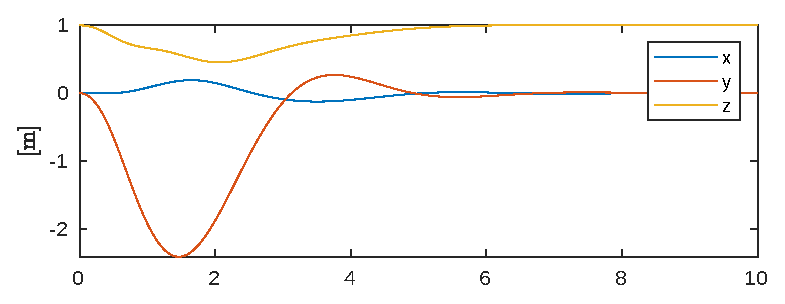
\includegraphics[width=0.8\linewidth]{fig/pos_edf}
    \caption{Posición del vehículo}
    \label{fig:pos_edf}
\end{figure}

\begin{figure}[!ht]
    \centering
    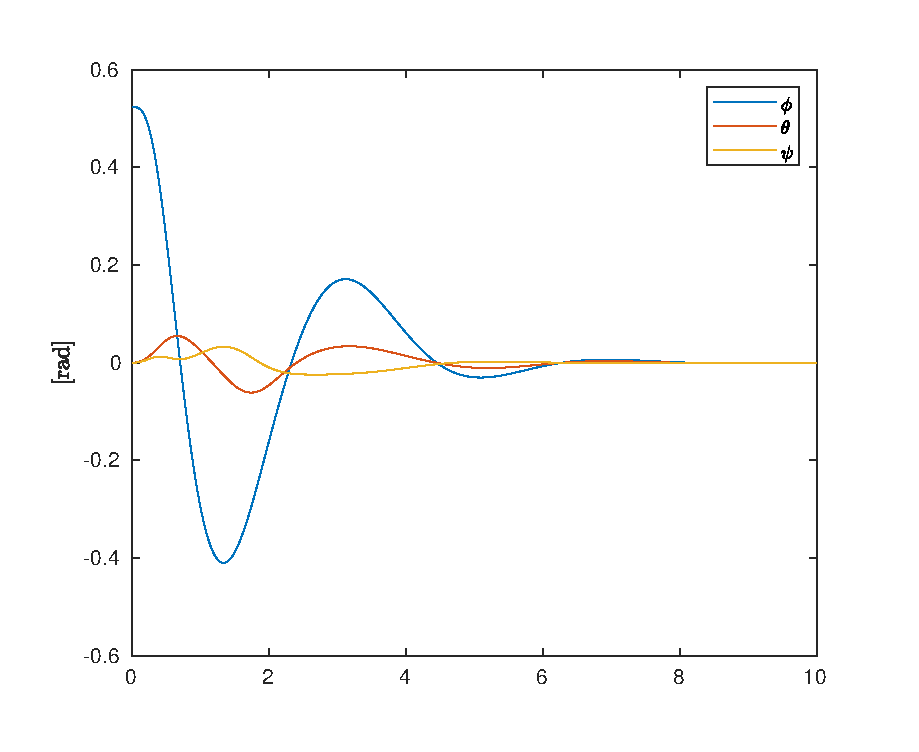
\includegraphics[width=0.6\linewidth]{fig/eulerang_edf}
    \caption{Ángulos de euler. Note que solo hubo perturbación inicial en $\phi$ sin embargo la actuación del gimbal ($\alpha$) generó una perturbación interna en $\theta$ por el efecto giroscópico.}
    \label{fig:eulerang_edf}
\end{figure}

\begin{figure}[!ht]
    \centering
    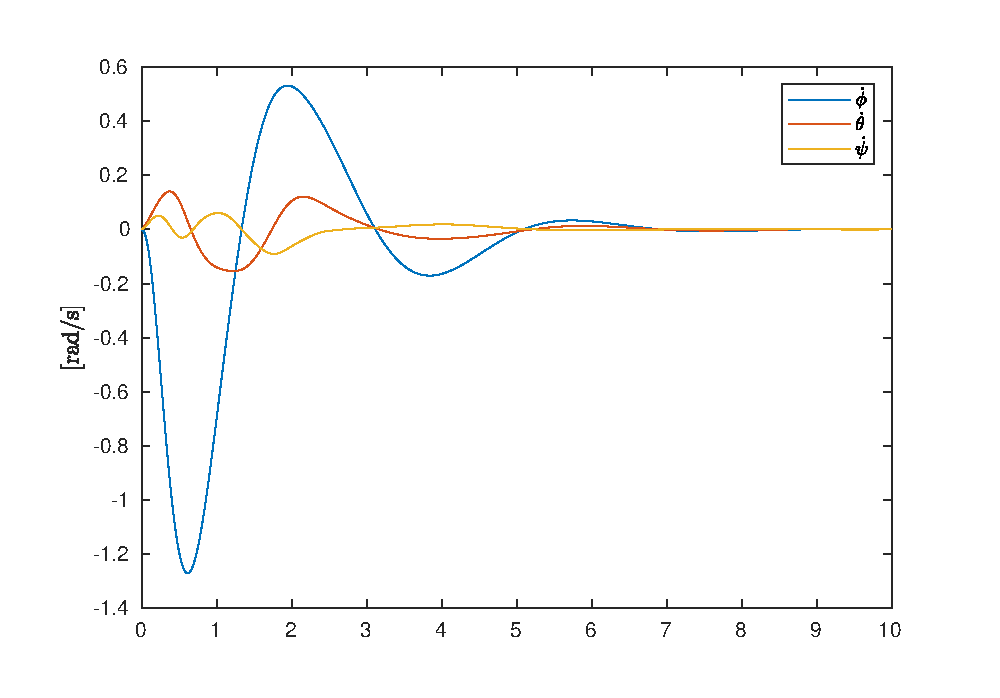
\includegraphics[width=0.6\linewidth]{fig/angvel_edf.eps}
    \caption{Velocidad angular del vehículo}
    \label{fig:angvel_edf.eps}
\end{figure}

\begin{figure}[!ht]
    \centering
    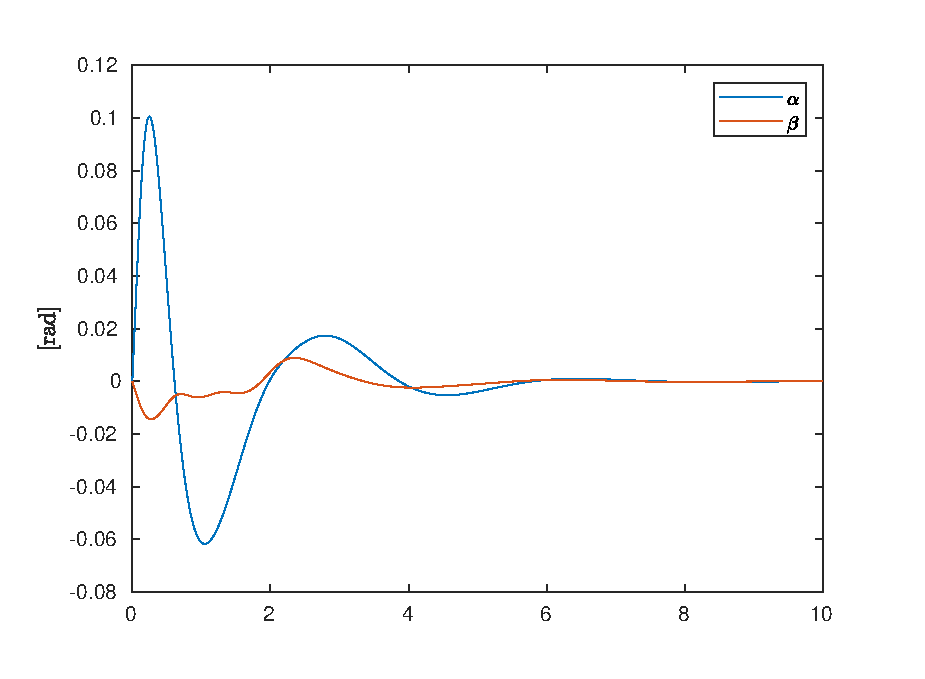
\includegraphics[width=0.6\linewidth]{fig/actuator_edf}
    \caption{Actuación angular del gimbal.}
    \label{fig:actuator_edf}
\end{figure}

\begin{figure}[!ht]
    \centering
    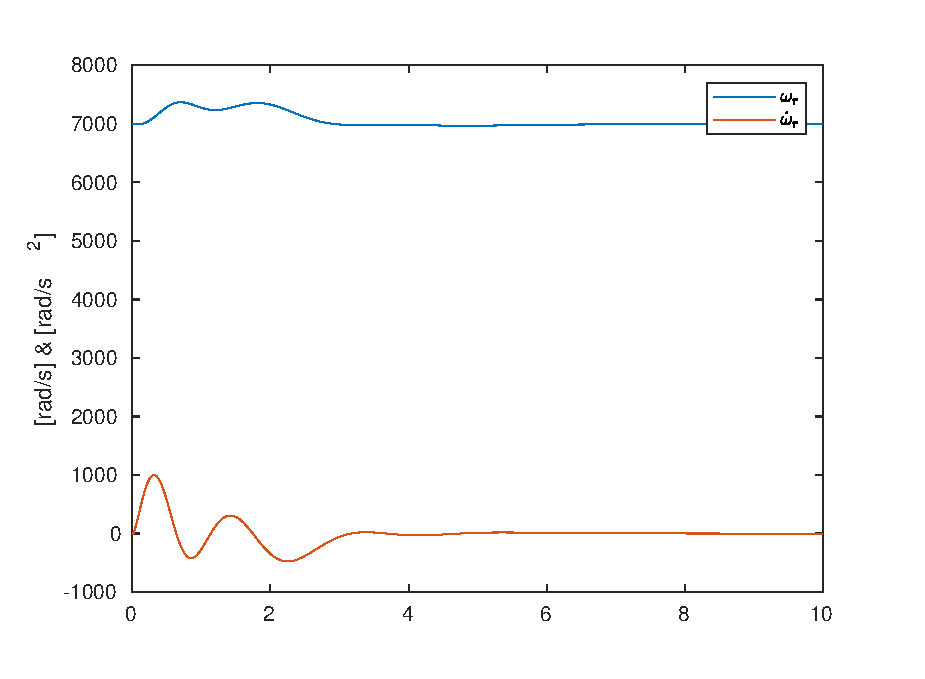
\includegraphics[width=0.6\linewidth]{fig/rotor_edf}
    \caption{Velocidad y aceleración angular del rotor.}
    \label{fig:rotor_edf}
\end{figure}





\null\newpage
\clearpage

\section{Desarrollo de software}

La decisión de software a utilizar dependió del controlador, poder de cálculo disponible, interfases de periféricos y funcionalidad deseada.

\medskip

Dado el uso de una Raspberry Pi,\footnote{La Raspberry Pi provee un entorno con Linux instalado que permite la programación con virtualmente cualquier lenguaje de programación en existencia.} el lenguaje de programación elegido fue \textbf{Go} (Golang) debido a los siguientes puntos

\begin{description}
    \item[Seguro] - Modelo de memoria Go, sistema de tipado fuerte\footnote{Hoy en día hay pocos lenguajes con sistemas de tipos fuertes. Contrario a la creencia popular, C y C++ ambos son tipados débilmente.}
    \item[Simple] - Claridad de sintaxis
    \item[Concurrencia] - Crear \glsplural{corrutina} es simple, paralelizar corrutinas es trivieal
    \item[Rendimiento] - Superior a Python, Java y Matlab. Comparable a C. Esto también implica un menor consumo de energía
    \item[Estable] - \textit{The Go 1 promise} (La promesa Go 1)
    \item[Comprobado] -  Usado en sistemas de alto-riesgo/alta-complejidad (Kubernetes, Docker, Go-HEP)
    \item[Portable] - Todos los programas Go compilan a código nativo (código de máquina) para cualquier arquitectura y sistema operativo. Incluso se puede programar microcontroladores (TinyGo)
\end{description}

\subsection{Flujo de control}
\begin{figure}[!htb]
    \centering
    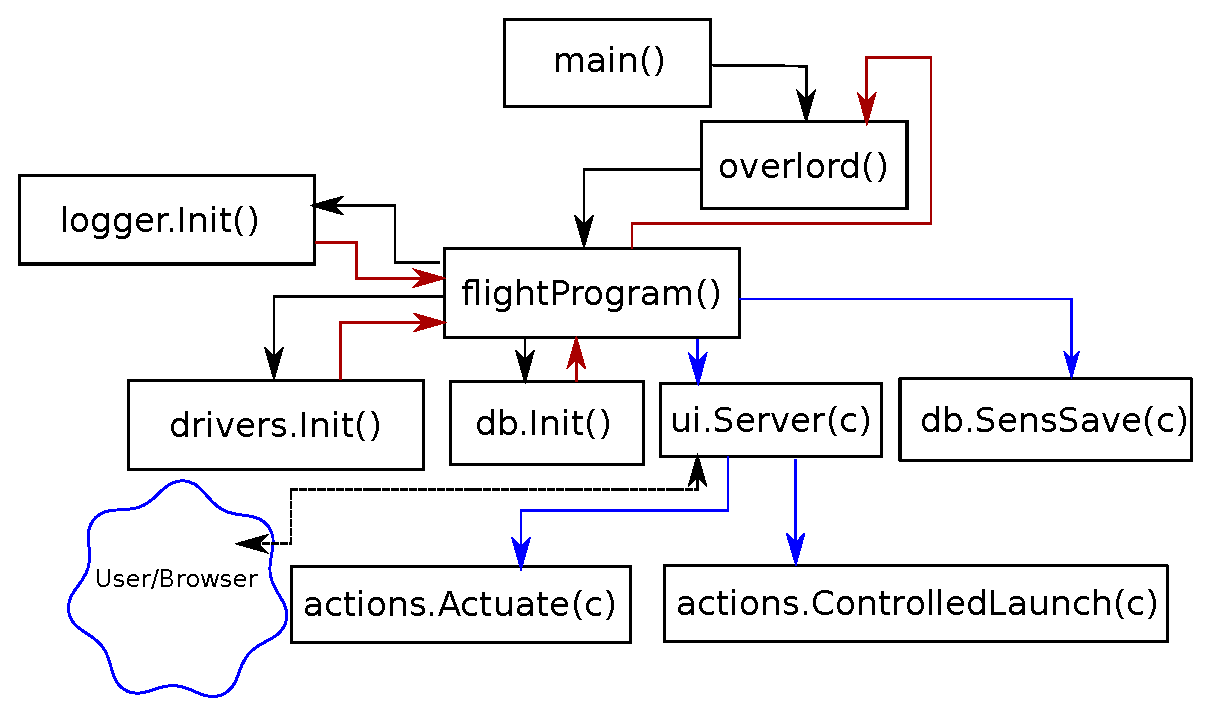
\includegraphics[width=0.7\textwidth]{fig/cfg_flightprogram.eps}
    \caption{Gráfico de flujo de control (CFG) del programa de vuelo. Las lineas de flujo azules son corrutinas independientes al programa principal. Las lineas negras son flujo del programa principal. Las lineas rojas son flujo del programa principal al encontrar un error.}
    \label{fig:flightProgram}
\end{figure}

Se ilustra el flujo de control a grandes rasgos usando un CFG en la figura \ref{fig:flightProgram}. El programa principal corrió la rutina \texttt{overlord} que a su vez comandó \texttt{flightProgram} y esperó que esta devuelva control a \texttt{overlord}. El propósito de \texttt{overlord} fue guardar el estado del vehículo y ante una falla irrecuperable en \texttt{flightProgram}, terminar con todas las corrutinas generadas por \texttt{flightProgram} y sus afiliadas y a su vez reiniciar \texttt{flightProgram} nuevamente con el último estado antes de la falla.


\subsection{Interfaz con hardware}

Como se mencionó anteriormente, la computadora elegida tiene varios puertos que sirviern como interfases con periféricos, entre ellos 

\begin{itemize}
    \item ADC (sensores)
    \item Generadores de PWM (para actuadores)
    \item Blinkenlights
\end{itemize}

Para la interacción del software con el hardware se usó la librería \href{https://periph.io}{periph.io}. Esta librería permitió la interacción a través de los puertos de comunicación de la Raspberry Pi. Los drivers para los periféricos fueron programados según la información dada en las datasheet.


\subsection{Implementación}

Al momento de escribir el presente informe el programa de vuelo tuvo 3540 líneas de lógica, de las cuales 1680 correspondieron a los drivers de control de periféricos. Se logró controlar la actuación de hasta 12 señales PWM y en simultaneo leer 16 señales de telemetría y guardar a archivo en una tarjeta SD a 1200 muestras por segundo (cada canal). 1060 líneas de código fueron dedicadas a la interfaz de usuario para facilitar el control del vehículo desde un browser, como por ejemplo Firefox.

\subsection{Debugging}

En junio 2021 se halló un bug en el software. Al cabo de cierto tiempo entraba en un estado degenerado el sistema donde no respondía a inputs de usuario ni a señales del sistema operativo. Debido a los periféricos usados la última señal mandada al actuador se quedaba fija y era imposible retornar el sistema a un estado seguro sin terminar el programa forzosamente y reiniciarlo. 

Se sospechaba que el bug era causa de una falla en el kernel de Linux para computadoras ARM o corrupción de memoria causada por el garbage collector de Go. Debido a la configuración de la computadora y las herramientas disponibles para Go era dificil debuggear. El debugger nativo de Go (Delve) no funcionaba aún en procesadores ARM de 32 bits y el detector de carreras de Go tampoco estaba disponible para procesadores ARM. Se pasó 6 meses investigando intermitentemente y hablando con expertos en software y hardware.

En enero 2022 se encontró el mismo comportamiento observado durante el bug mientras se desarrollaba un proyecto no asociado a este trabajo. En este software el estado degenerado era causado por una condición de carrera, específicamente era el caso de una \gls{datarace}. Con este conocimiento se modificó el programa de vuelo para que pueda correr en un entorno de computadora desktop. Para lograr esto se programó un mock de la escritura I2C que fue facilitado por el uso de \textit{interfaces} en Go. Esta modificación permitió al detector de carreras de Go encontrar condiciones de carrera en el programa de vuelo. Se encontraron y se arreglaron 2 condiciones de carreras causadas por error de programador debido al uso equivocado de mutexes.

Aún así el error persistía y el programa seguía encontrandosé en el estado degenerado. Se optó por reescribir el programa de cero y aplicando patrones de diseño más estrictos y seguros. Al cabo de un mes se había reescrito el programa de vuelo de la empresa y el bug no volvió a resurgir en el desarollo. Esto se puede deber a que se redujo el uso de librerias de terceros y la cantidad de líneas de código totales bajó de 700.000 a tan solo 30.000, incluyendo dependencias de terceros3. Excluyendo las liberías de terceros, la base de código era de tan solo 2100 líneas e incluía el frontend (interfaz con el usuario).



\null\newpage
\clearpage


\section{Pruebas}

Se probó el prototipo en las instalaciones de LIA Aerospace. Para esto se colgó de 3 puntos de anclaje con sogas para poder lograr que quede sin estar en contacto con el suelo a una distancia de aproximadamente 1 metro, colgado en el aire, para que en caso de suceder algún desperfecto o salida de control el prototipo no colisione abruptamente con alguna superficie que no sea la indicada, el tren de aterrizaje.

En las pruebas lo que se buscaba era lograr una maniobra Hopper, esto es, un despegue y aterrizaje vertical, combinado con un desplazamiento direccional con el vehículo orientado verticalmente.

Se iniciaba y se terminaba suspendido en el aire porque el software de vuelo estaba siendo desarrollado aún y los parámetros estaban siendo modificados.
Se puso una soga atada directamente al prototipo para que en caso de una emergencia o salirse de control, tener una posibilidad de guiar el vehículo a mano.


\null\newpage
\clearpage

\section{Desafíos y soluciones}\label{sec:challenges-solutions}

\subsection{Fallo de programa de vuelo}
Durante una prueba de campo el prototipo entró en un estado degenerado. Esta fue una situación donde el ruido del EDF no permitía la comunicación verbal entre el equipo presente, aún estando a 3 metros de distancia. Se encontraban 2 operadores en el lugar, uno manejando el control del vehículo a través de la interfaz gráfica y otro operador manejando la soga que prevenía que el vehículo vuele más alto de 3 metros como se había convenido.

Comenzó con un momento de confusión cuando luego de comandar a que se detenga el EDF no se detuvo. El operador de la interfaz intentó recuperar el control a través del fail safe pero esto tardaba varios segundos. Mientras tanto el operador de la soga no se enteró de la falla y dejó que el vehículo se acerque al límite de los 3 metros. Al no detenerse el motor como se venía haciendo el vehículo pegó un tirón y al inclinarse comenzó la pérdida total de control de la situación mientras el EDF comenzaba a agregar energía a los movimientos rotacionales del vehículo. Esto último sucedió en menos de 3 segundos. Luego el operador de la soga procedió a realizar una secuencia de apagado forzoso a mano. Para lograr esto había que acercarse al dispositivo, lograr capturarlo y apagarlo manualmente.

Durante esta maniobra una soga se metió por la admisión del EDF provocando la rotura crítica del EDF. El EDF en este momento estaba girando por encima de las 30.000 vueltas por minuto, provocando que se desprendan partes de aluminio de los álabes. De esta forma quedó desbalanceado rotando a decenas de miles de vueltas por minuto haciendo un ruido que podría ser descrito como ``ensordecedor". El operador de la soga igual pudo acercarse al dispositivo y desconectar el enchufe de las baterías que estaba en un lugar de difícil acceso. Tuvo que abrazar al dispositivo con los codos y utilizar las manos para desconectar la batería.

Esta situación trajo algunas mejoras con respecto a la seguridad:

\begin{itemize}
    \item Una señal visual para cuando las cosas se salen de control y activar un protocolo de emergencia.
    \item Protección completa en los brazos
    \item Una rejilla en la admisión del EDF para que no pueda succionar por error algún objeto.
    \item Un cortacorrientes más accesible para un apagado de emergencia.
    \item Un rediseño para el anclaje en el lugar de ensayo.
    \item Una corrección del bug de software para evitar que el prototipo entre en un estado degenerado en el que no responde a ningún comando, ni siquiera los supremos de Linux.
\end{itemize}

\subsection{Rediseño de sistema de flaps}

Cuando se estaba realizando la etapa de diseño, se debía realizar la implementación de flaps antirrolido. Estos flaps tienen como misión desviar el flujo proveniente del EDF para obtener como resultado un control de rolido. Se realizó el diseño en CAD en una etapa temprana del proyecto, con la guía de planos del fabricante que se consiguieron por internet. Estos planos no contenían el nivel de detalle que permitieran conocer que parte rotaba por su superficie externa, para poder realizar el diseño previo de todo el proyecto antes de que se logren importar todas las piezas aledañas. Se prototipo la pieza que contenía los ejes de los flaps simplemente apoyados, para poder ser fabricada con manufactura aditiva en una impresora 3D con PLA. Se procedió a realizar la pieza y tenerla lista a la espera de la importación del EDF. Cuando el EDF y las piezas faltantes ingresaron a suelo argentino, y se procedió con el armado, se detectó que el anillo contenedor del apoyo de los flaps que había sido diseñado anteriormente, apretaba sobre una pieza móvil del EDF, que no había sido especificada en los planos. Esto llevó a tener que realizar un rediseño completo de flaps y apoyos, con un diseño mucho más complejo al tener algunas piezas ya fabricadas que imponían condiciones bastantes dificultosas para que todo encaje y tenga un accionar correcto del mecanismo antirrolido.

\medskip

Cuando se probó el sistema antirrolido, los microservos que accionaban el mecanismo de los flaps, dejaron de funcionar, esto sucedió debido a que la caja de engranajes era de plástico y la calidad de este componente no era acorde al tipo de proyecto y utilización que se estaba llevando a cabo. Según los datos del fabricante esta pieza estaba en especificación para la utilización que le estábamos dando, pero las prácticas determinaron que esto no era así. Esta situación llevó a tener que cambiarlos por unos servos con caja de engranajes de metal y salida estriada de metal para el accionar del mecanismo flap antirrolido. Como así también un rediseño de los anclajes de la envuelta de los servomotores.

\subsection{Problemas electricos}
Durante las pruebas fue común observar que al conectar las baterías la computadora de vuelo se apague debido al arc flash que ocurriía adentro del conector. Esto se debía a la alta capacitancia
del \gls{esc} que contiene un banco de capacitores grande. Para subsanar la situación se fabricó un echufe de dos etapas donde el primer contacto permitía cargar los capacitores a traves de un termistor NTC. El termistor tenía una resistencia de miles de ohms nominal que bajaba al momento que comenzaba a circular corriente. Esto permitía cargar los capacitores rápido y de forma segura.

Además del arc flash en varias ocasiones se quemaron salidas digitales optoacopladas de la computadora de vuelo. Resultó aparente que se requerían de componentes de protección adicionales.
Se optó por diseñar la PIAA (sección \ref{ssec:electronicsdesign}) como solución duradera que soportara el entorno hostíl. Para subsanar la situación de forma inmediata se utilizaron salidas digitales que no habían sido quemadas y se les soldaron diodos zener de 9V de protección. Además se puso un optoacoplador secundario para controlar la ESC. Este último optoacoplador iba montado sobre un zócalo que permitía el fácil intercambio ante otra falla.

\null\newpage
\clearpage

\section{Conclusión}\label{sec:conclusion}

Como hemos podido apreciar en el presente informe, luego del análisis de cada sistema por separado, el diseño, desarrollo y construcción de cada subconjunto, se pudo lograr la implementación de un software de control escrito enteramente por nosotros adaptado a un vehículo físico, autonomo con tecnlogía VTVL, construido por un equipo de dos estudiantes. Se pudo comprobar el cumplimiento de los requerimientos propuestos al inicio de este proyecto.

% Esto culminó en las pruebas que mostraron que se cumplieron los requerimientos propuestos al inicio del proyecto.

\medskip

El proyecto tuvo dificultades complicadas de sortear debido a que este tipo de tecnologías no es frecuente, ni sencilla, existe solo una empresa en todo el mundo que logró la implementación exitosa a escala mayor y utiliza como medio para completar comercialmente las misiones. No existen antecedentes en instituciónes académicas de libre acceso que permitan una guía o referencia para llevar a cabo un proyecto de similares características. Hasta donde se pudo averiguar no se encontraron casos similares.

% Cada subconjunto podría haber sido un proyecto final, teniendo en cuenta el costo, y el tiempo disponible en un proyecto final de carrera en el ITBA.

Se destacan la utilidad de las herramientas de software que supimos poder dominar durante la carrera, tanto el uso del CAD que permitió facilitar la construcción y caracterización del vehículo en tiempos de pandemia que nos obligó a trabajar separados, y poder llegar dentro de los plazos estipulados con una aproximación de diseño. Que luego fue evolucionando hasta su forma casi final en la etapa temprana del proyecto. Logrando continuar con una construcción pasando por múltiples procesos productivos, que culminaron en la producción de piezas idénticas a las que están en la pantalla. Cuando se comenzaron las tareas de ensamble e integración, las piezas fueron integradas al vehículo sin mayores inconvenientes debido a la precisión manejada por el software. También se menciona la utilización del modelado de elementos finitos, que nos proporcionó la información necesaria para poder verificar una geometría. Es importante destacar que este tipo de herramientas nos permitió la comunicación eficiente con documentación clara y concisa. Teniendo condensado en una imagen o gráfico lo necesario para tomar una decisión de diseño para luego poder tener un éxito en la misión.

\medskip

Se destaca también, que se aprendió que, en los proyectos de ingeniería de tal complejidad, es un acierto invertir tiempo en las decisiones en las etapas tempranas. Diseñando, simulando, discutiendo la funcionalidad e implementación de piezas caras y complejas. Esto permite corregir a tiempo antes que se invierta tiempo y dinero en diseños que no habían nacido correctamente y que por más que se optimicen en un futuro el problema es más profundo a tal punto de determinar que una pieza no es necesaria.

Se pudo lograr entrar dentro del presupuesto diseñando piezas para ser construidas en máquinas tradicionales. Se dejó de lado la utilización de un control numérico de varios ejes. Este proyecto puede ser replicado con un torno y una fresa, además de herramientas manuales cotidianas. Esto se logró pensando la pieza desde varios frentes, no solo de forma funcional, sino como así también las herramientas que había a disposición y el costo asociado a las horas, tan simple como se pueda.

Las pruebas de campo otorgaron resultados positivos, pese al incidente hablado en la sección \ref{sec:challenges-solutions}. Se pudieron sortear los distintos problemas para controlar y realizar vuelos exitosos mediante la implementación del software de vuelo en el dispositivo que se construyó. Produciendo un despegue y aterrizaje exitoso. Esto se logró utilizando en gran parte componentes comercialmente disponibles, esto es a excepción de las piezas custom que teníamos la capacidad de volver a proveer rápidamente si fuera necesario. Se pudieron conseguir nuevamente las partes
que se rompieron para continuar con el presente trabajo. Por esto es que los componentes COTS fueron vitales para poder comprobar una hipótesis y no quedar en el camino demorado o estancado por fallas. Eventualmente el hardware traerá problemas.

El ingeniero aeroespacial a cargo del sistema de control del prototipo FROG de la ESA, Stéphane Querry de Polyvionics, dio su aprobacion del proyecto luego de una conversación con el equipo acerca los algoritmos de control.
Lo que generó el conocimiento acerca del proyecto en Stephane fue de tal magnitud que stephane ofrecio ser mentor en el desarrollo de software. Después de recibir una presentación del proyecto, Stéphane se mostró dispuesto a brindar su experiencia como mentor en el desarrollo del software. Esto fue aprovechado varias veces en la forma de reuniones virtuales donde se hicieron preguntas a Stéphane acerca temas de GNC para trabajos similares en LIA Aerospace. En varias ocasiones Stéphane verbalizó incredulidad amistosamente acerca el hecho que un proyecto como el presente estaba siendo llevado adelante por dos personas.

% Lo que generó el conocimiento acerca del proyecto en Stephane fue tal que el mismo ofrecio ser mentor en el desarrollo de software. 

\medskip

Haber trabajado sobre este proyecto nos permitió crecer en el ambiente aeroespacial y poder solucionar problemas similares en el día a día. Las equivocaciones en el trayecto hasta la finalización del prototipo o la frase “esto podría estar mejor” salieron a la luz para ser solucionadas posteriormente. Es algo no menor en el trabajo de un casi ingeniero trabajando en la mesa de diseño cuando las características del proyecto no admiten equivocaciones.

Para culminar, estamos orgullosos y felices de poder aportar un granito de arena con el desarrollo de comienzo a fin de tecnologías que permitirían la realización de vuelos espaciales suborbitales e incluso orbital con el escalado del prototipo.

Por nuestra parte esperamos poder fomentar y alentar a que se puedan seguir generando documentos e investigaciones sobre este tipo de tecnologías en la institución, siendo que no habían antecedentes, más allá de las limitaciones geo espaciales, económicas, las barreras de importación u opiniones acerca de la complejidad, cuando se trabaja en equipo y con pasión las misiones se pueden lograr.


\section{Trabajo a futuro}

Se detallan puntos que se consideran importantes para continuar con el desarrollo del la tecnología propuesta en el presente trabajo e incluso para poder escalar el proyecto a un nivel mayor.

\begin{itemize}
    \item \textbf{Estimación de actitud:} El estimador usado fue un filtro Madgwick. A futuro sería deseable implementar un filtro de Kalman, que es un estimador de estado óptimo. Esto permitiría obtener una estimación de actitud más robusta ante perturbaciones.
    \item \textbf{Rack de componentes:} Se podría implementar la idea de colocar una pieza contenedora de todos los componentes electrónicos para poder quitarlos y ponerlos de forma rápida a modo de rack. Esto además permitiría realizar pruebas de la electrónica y modificaciones de forma más eficiente.
    \item \textbf{Mejora en la seguridad y fiabilidad:} Se podrían implementar sistemas de seguridad para garantizar un vuelo seguro y confiable. Esto incluiría la integración de redundancias y sistemas de respaldo para mitigar posibles fallos y minimizar el riesgo de accidentes.
    \item \textbf{Integración de tecnologías de machine learning:} La integración de tecnologías de machine learning podrían proporcionar mejoras significativas en el rendimiento del VTVL autónomo. Los sistemas de machine learning podrían ayudar en la toma de decisiones autónomas, el reconocimiento de obstáculos, la planificación de rutas óptimas y la optimización de las maniobras de vuelo.
    \item \textbf{Utilización de sensores de alta calidad:} Los sensores utilizados tienen decadas de uso en la industria. Ya hay sensores de mejor calidad y más precisos que podrían ser utilizados para mejorar la estimación de estado.
    \item \textbf{Sensado absoluto de posición: } Se podría implementar un sistema de sensado absoluto de posición para mejorar la estimación de estado. Esto podría ser un sistema de GPS, un sensor laser funcionando por principio de Time-of-Flight sistema de visión de maquina.
\end{itemize}

\null\newpage
\clearpage

\subsection*{Agradecimientos}
Dan Etenberg por habernos ayudado en condiciones dificiles dado el contexto de pandemia y por proveer instalaciones, compra de materiales e insumos. 

\medskip

Stéphane Querry por haber intercambiado información acerca de parámetros de diseño del proyecto FROG de la ESA relevantes a la programación del sistema de control.

\medskip

Pablo Cossutta por compartir su experiencia trabajando con sistemas de potencia electrónicos. 

\null\newpage
\clearpage

\section{Anexo}

\subsection{Diseños preliminares - imágenes}

\begin{figure}[htb]
    \centering
    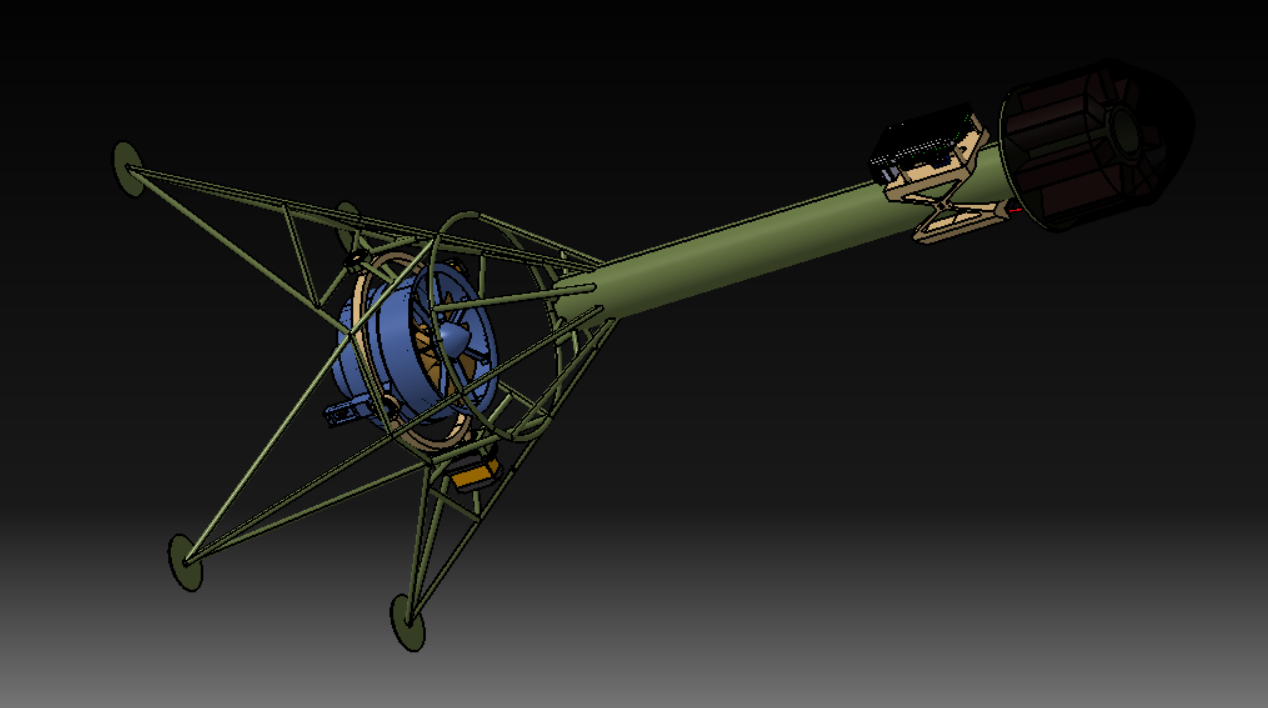
\includegraphics[height=0.25\pdfpageheight]{fig/design/0}
    \caption{Prototipo de fuselaje con patas reticuladas integro en aluminio, baterías en la nariz, aviónica debajo de la nariz, sin sistema anti rolido.}
    \label{fig:design/0}
\end{figure}


\begin{figure}[htb]
    \centering
    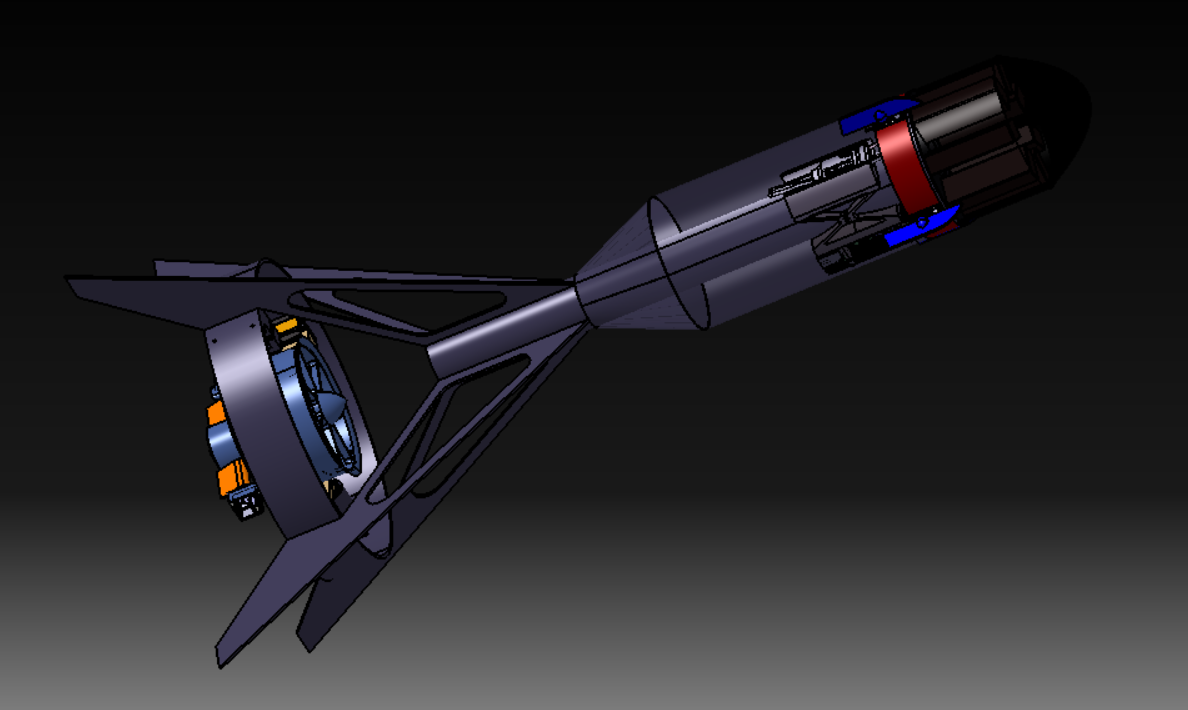
\includegraphics[width=\linewidth]{fig/design/1}
    \caption{Prototipo evolución al fuselaje de aluminio tubular, baterías en la nariz, sistema anti rolido en
    la parte superior, aviónica debajo de las baterías.}
    \label{fig:design/1}
\end{figure}

\begin{figure}[htb]
    \centering
    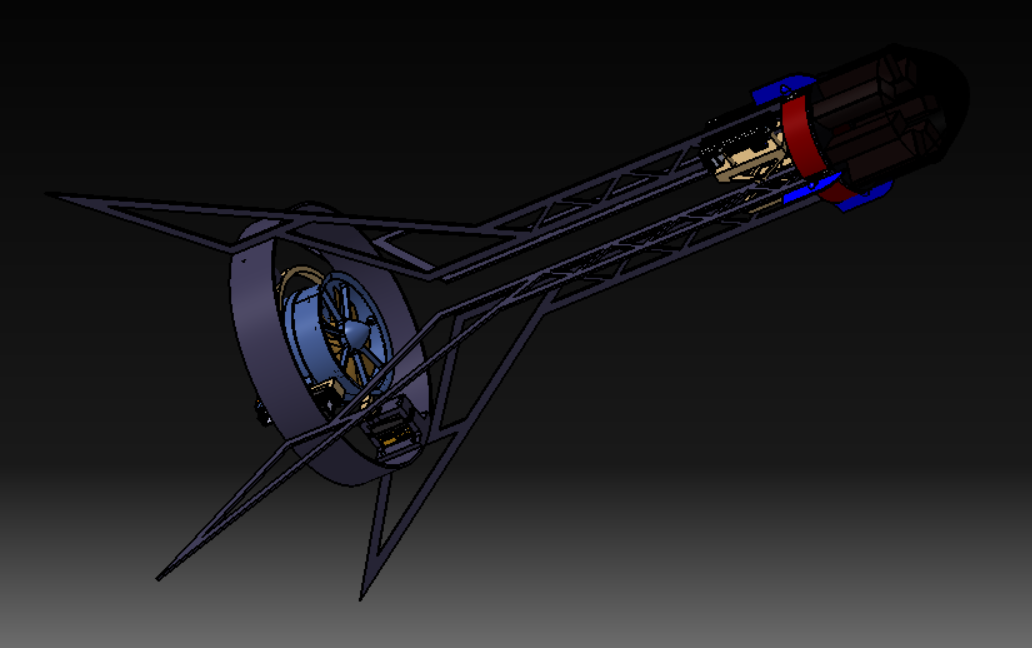
\includegraphics[width=\linewidth]{fig/design/2}
    \caption{Prototipo fuselaje reticulado de aluminio en forma de placas, baterías en la nariz, sistema anti
    rolido en la parte superior, aviónica debajo de las baterías.}
    \label{fig:design/2}
\end{figure}

\begin{figure}[htb]
    \centering
    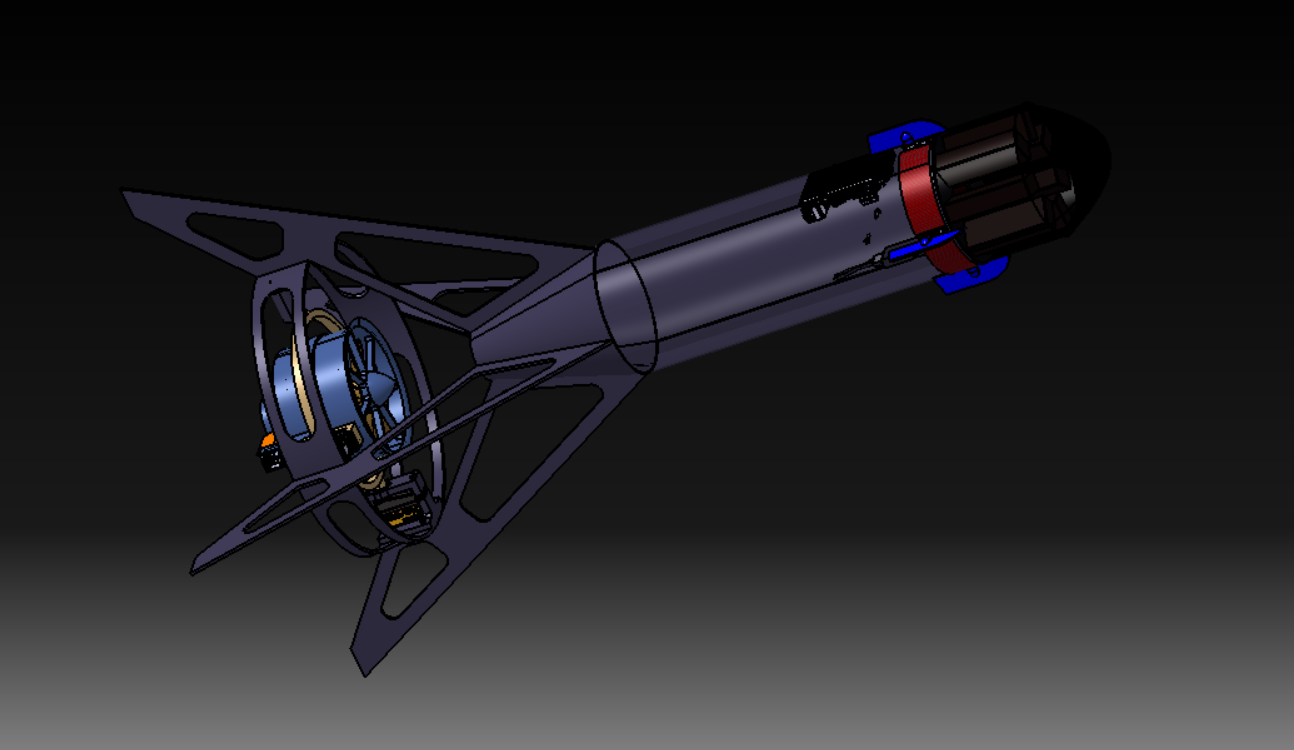
\includegraphics[width=\linewidth]{fig/design/3}
    \caption{Prototipo fuselaje tubular conico, para favorecer la admision del EDF, patas vaciadas, beterias en la nariz, siste a antirolido eb la parte superior,  avionica por debajo de las baterias.}
    \label{fig:design/3}
\end{figure}

\begin{figure}[htb]
    \centering
    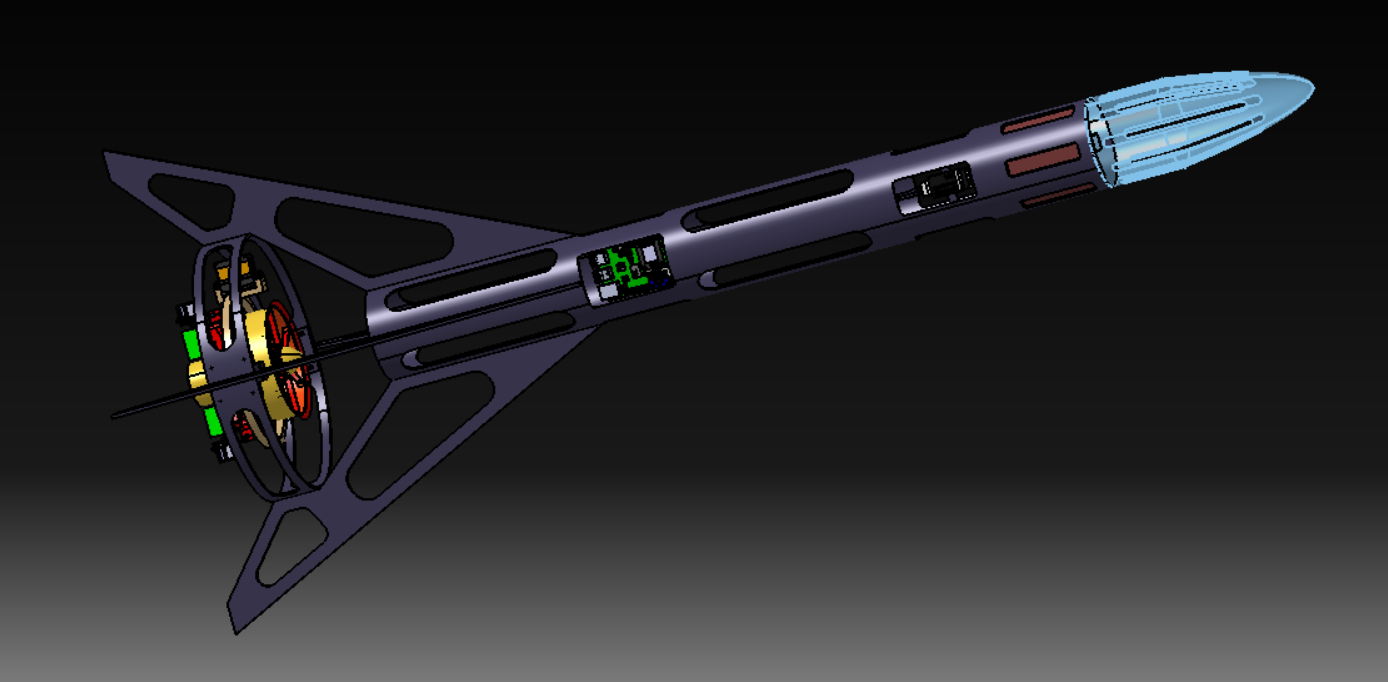
\includegraphics[width=\linewidth]{fig/design/4}
    \caption{Un diseño previo al diseño final. Los vaciados son distintos y la disposición de componentes es distinta. La posición de la Raspberry Pi fue cambiada luego de la charla con Pablo Cosutta.}
    \label{fig:design/4}
\end{figure}

\begin{figure}[htb]
    \centering
    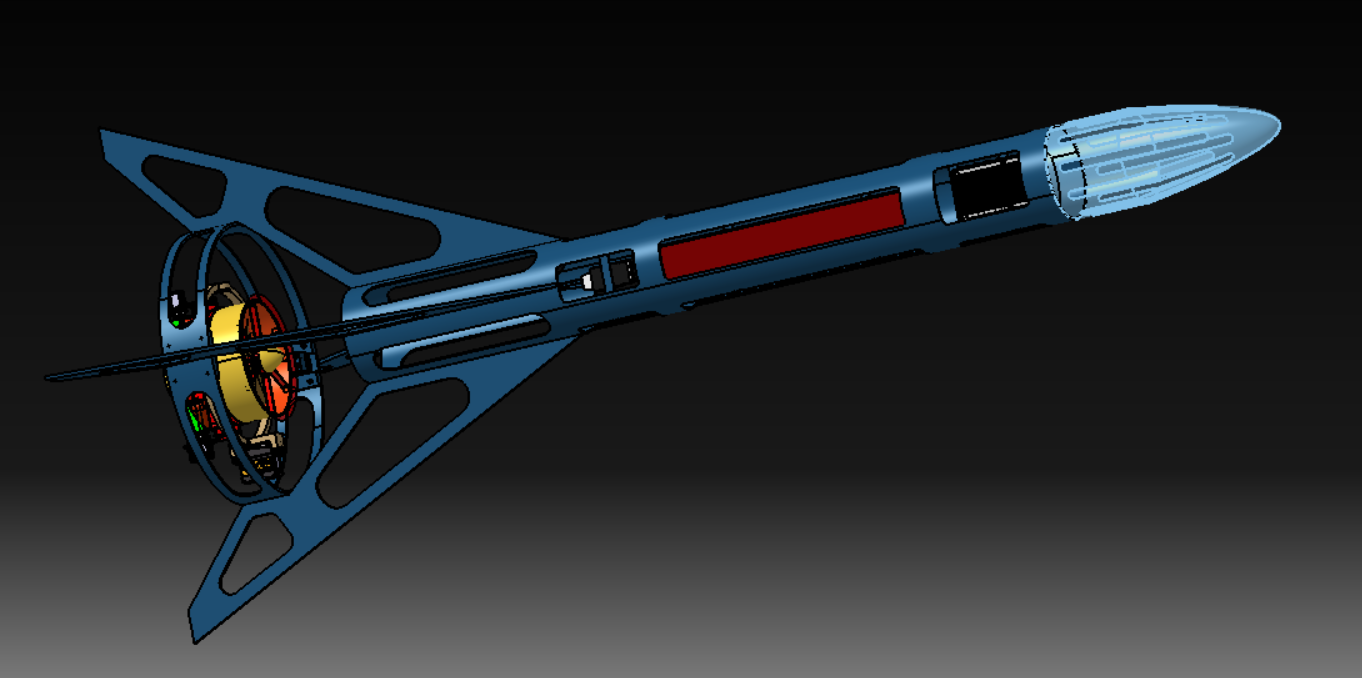
\includegraphics[width=\linewidth]{fig/design/5}
    \caption{Prototipo fuselaje de aluminio tubular vaciado, baterías en el cuerpo, en el núcleo, nariz aerodinámica, patas optimizadas, aviónica en la parte superior, sistema anti-rolido en la parte
    inferior del EDF por derivación del flujo.}
    \label{fig:design/5}
\end{figure}

\null\newpage
\clearpage


\bibliography{tex/biblio} % Indica archivo
\bibliographystyle{plainnat} %estilo de bibliografía
% \bibliographystyle{unsrtnat}
%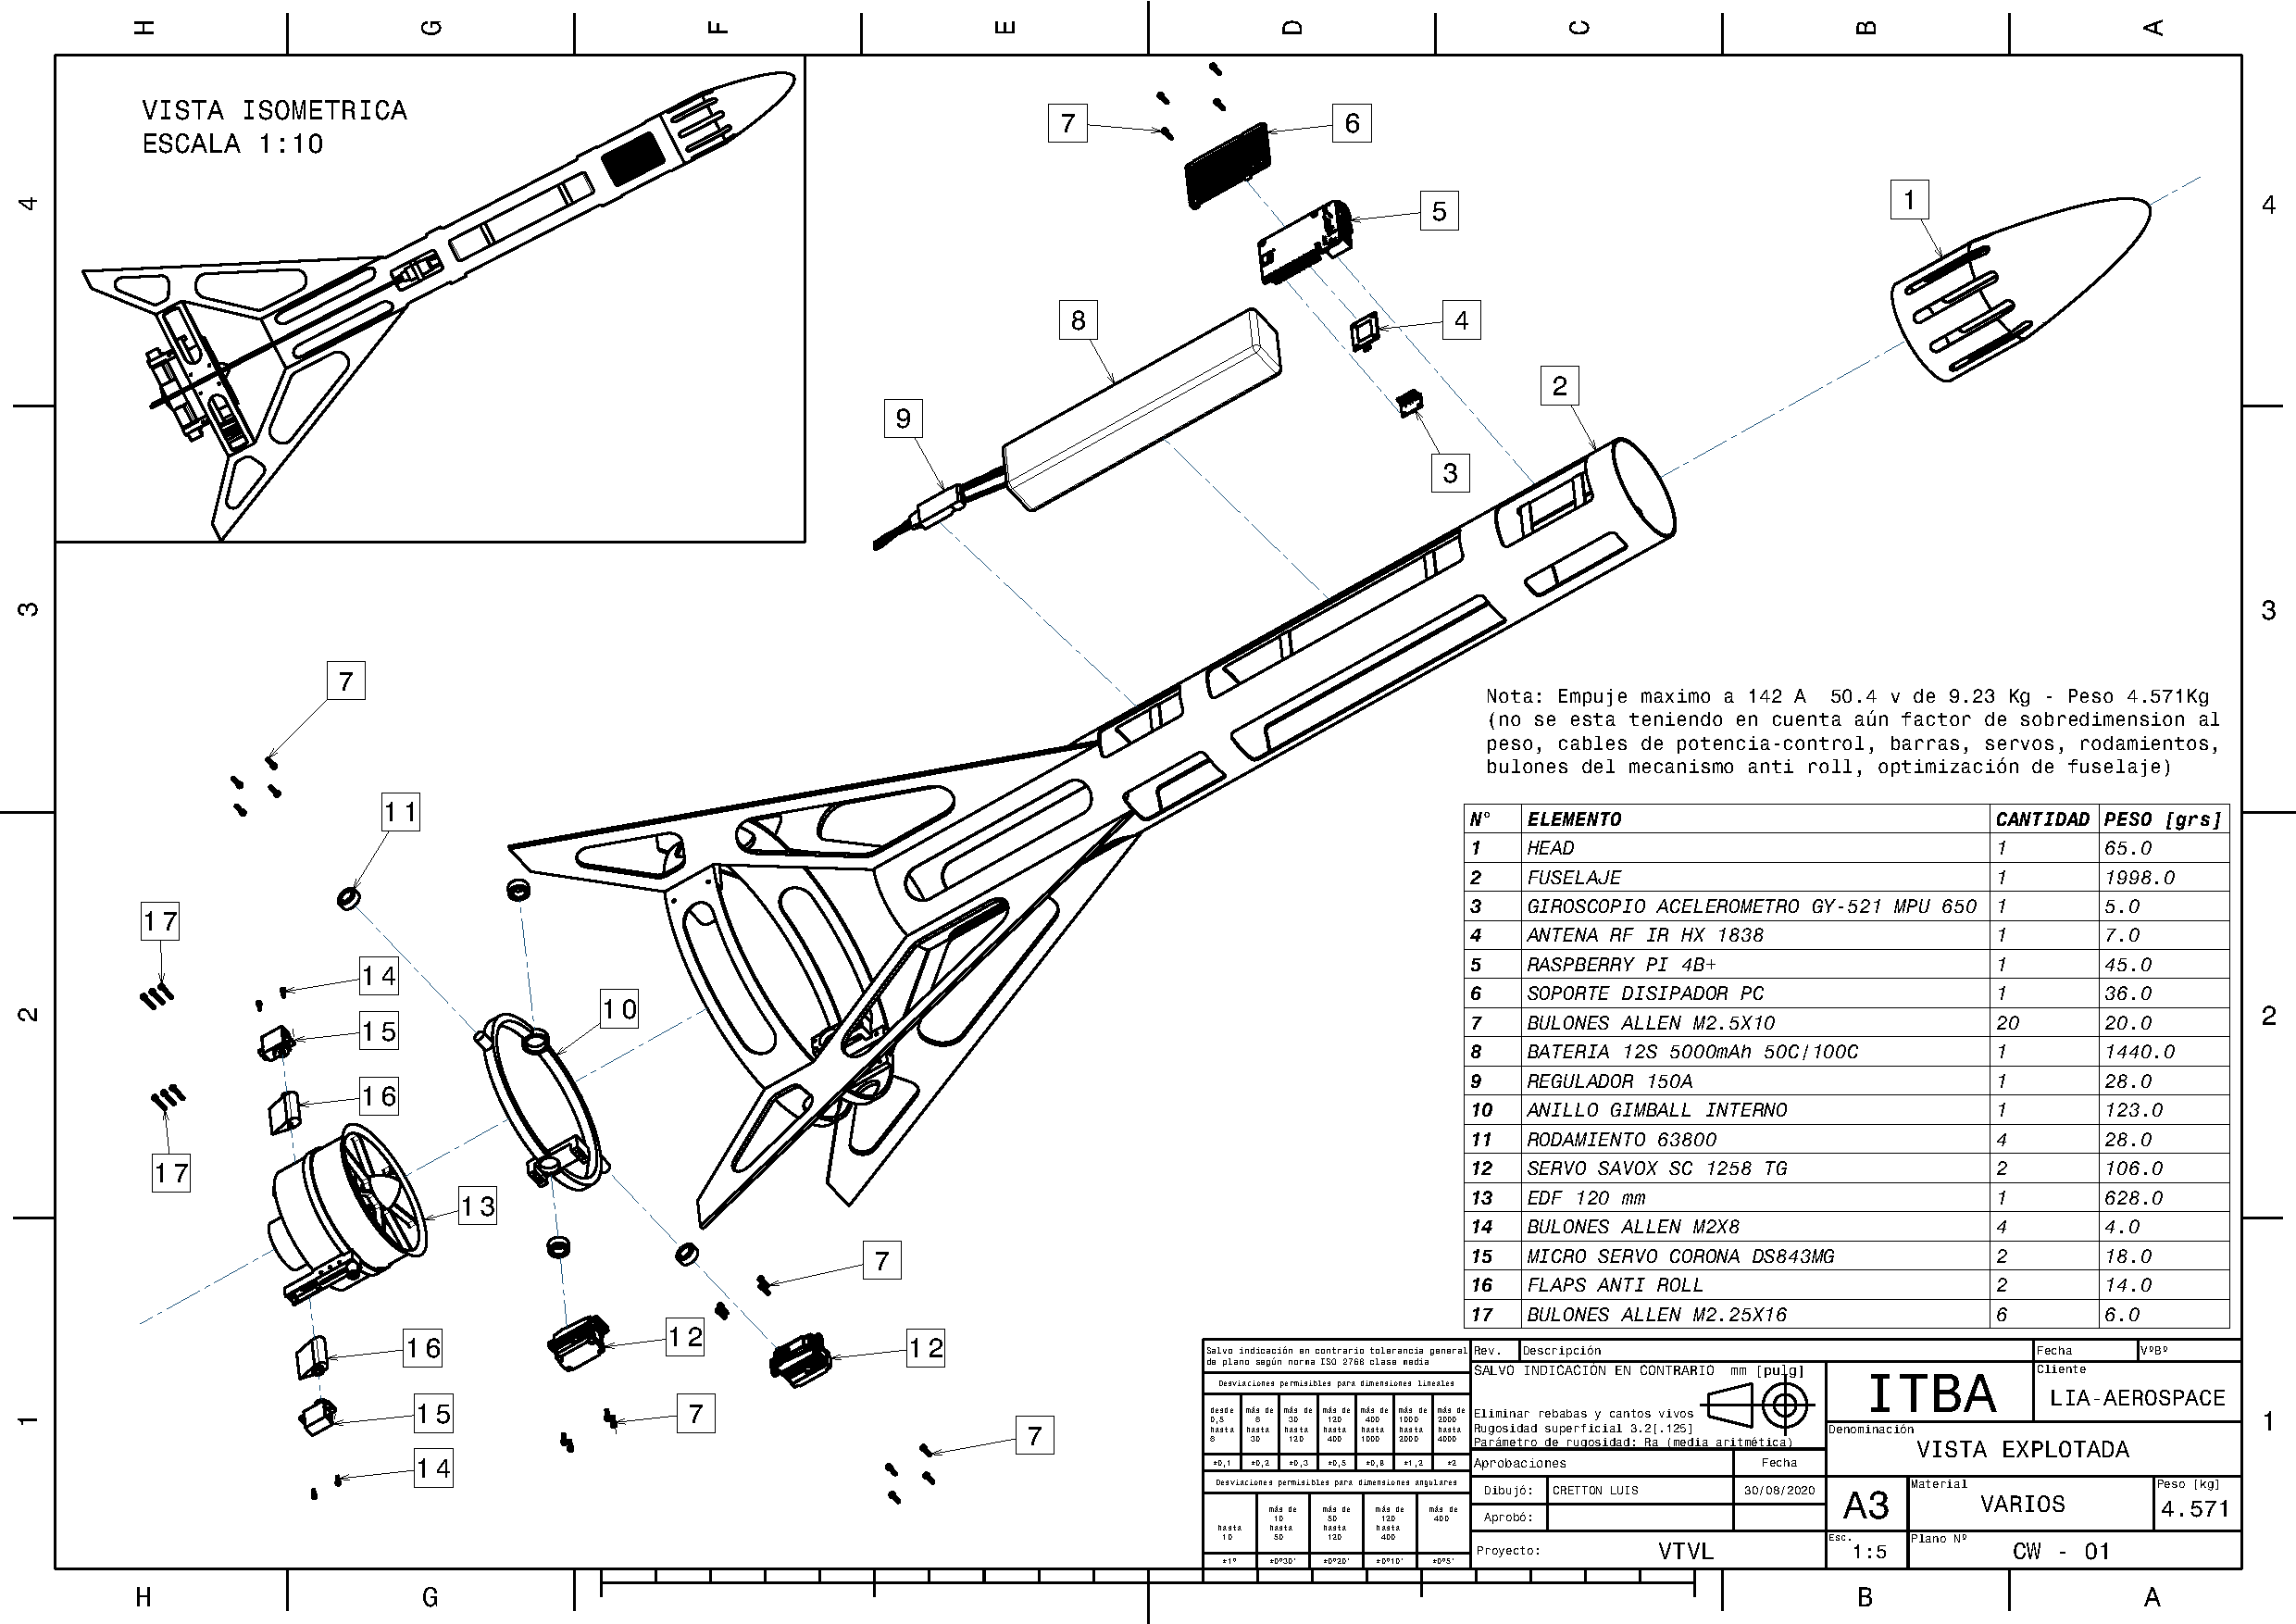
\includepdf[fitpaper=false,landscape]{pdf/Vistaexplotada5.pdf}

\null\newpage
\clearpage

\section{Secuencia de evolución del prototipo}
% VIEJAS
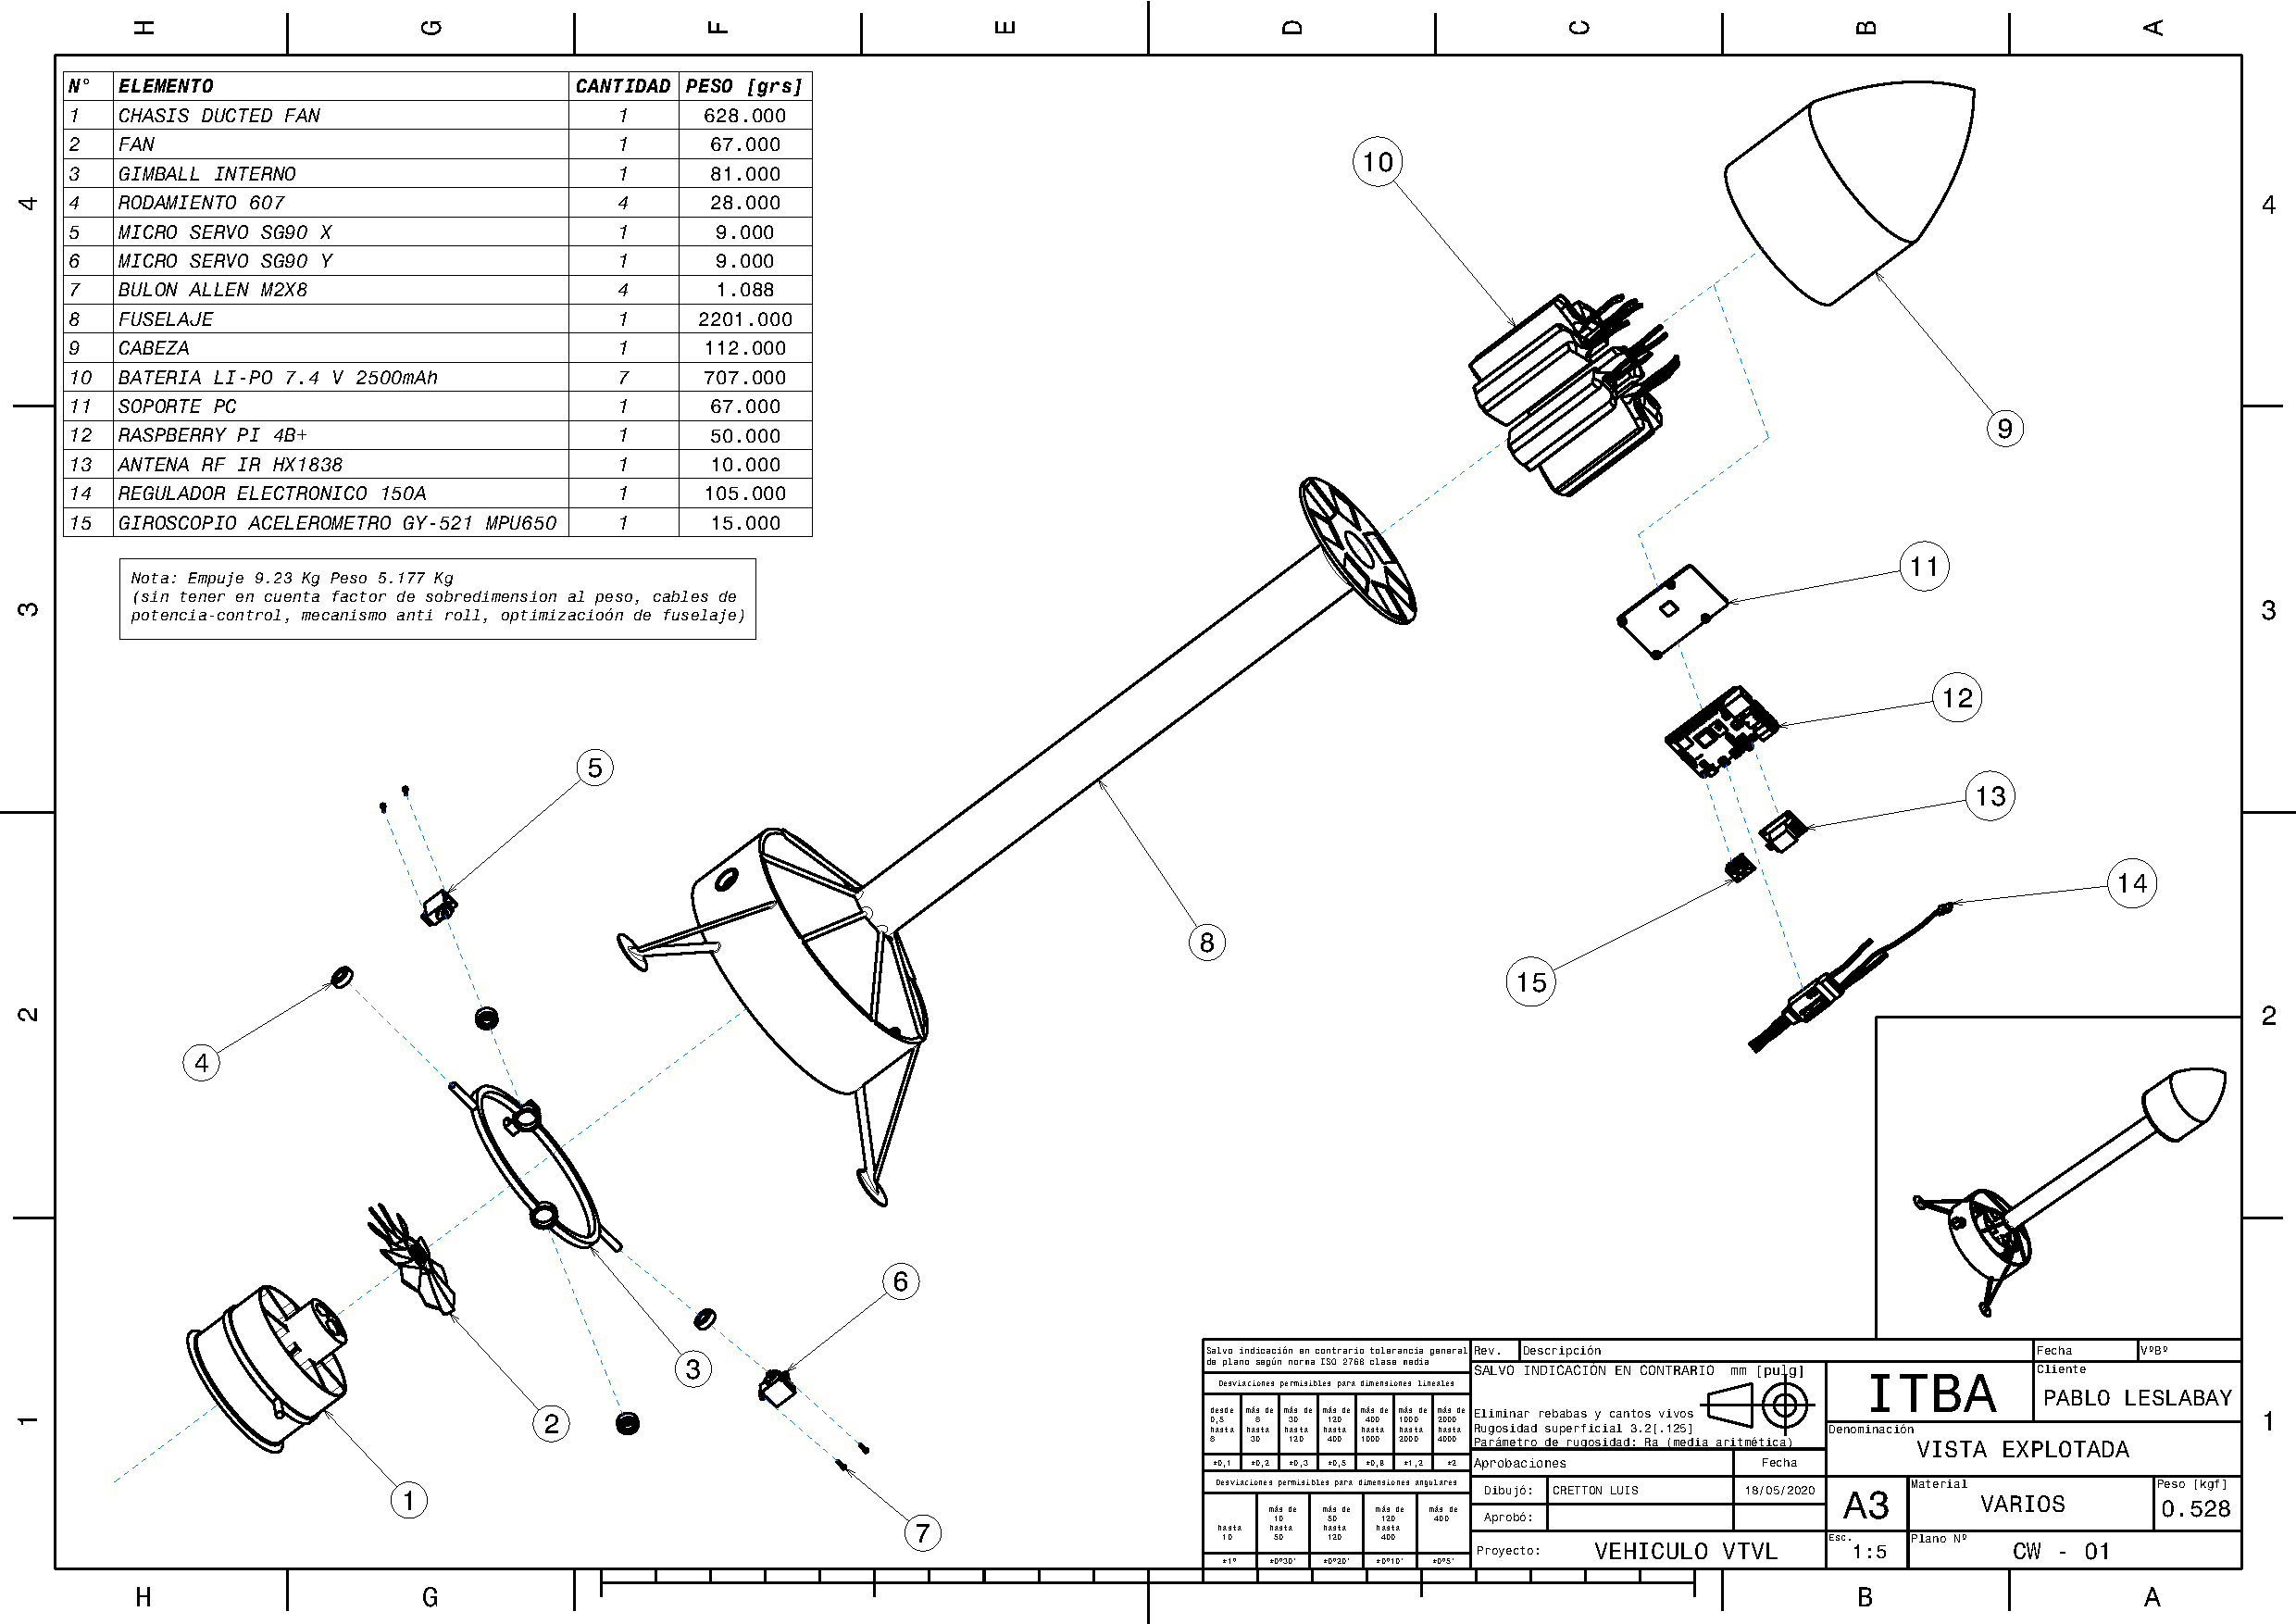
\includepdf[angle=90]{pdf/cad/Vista explotada}
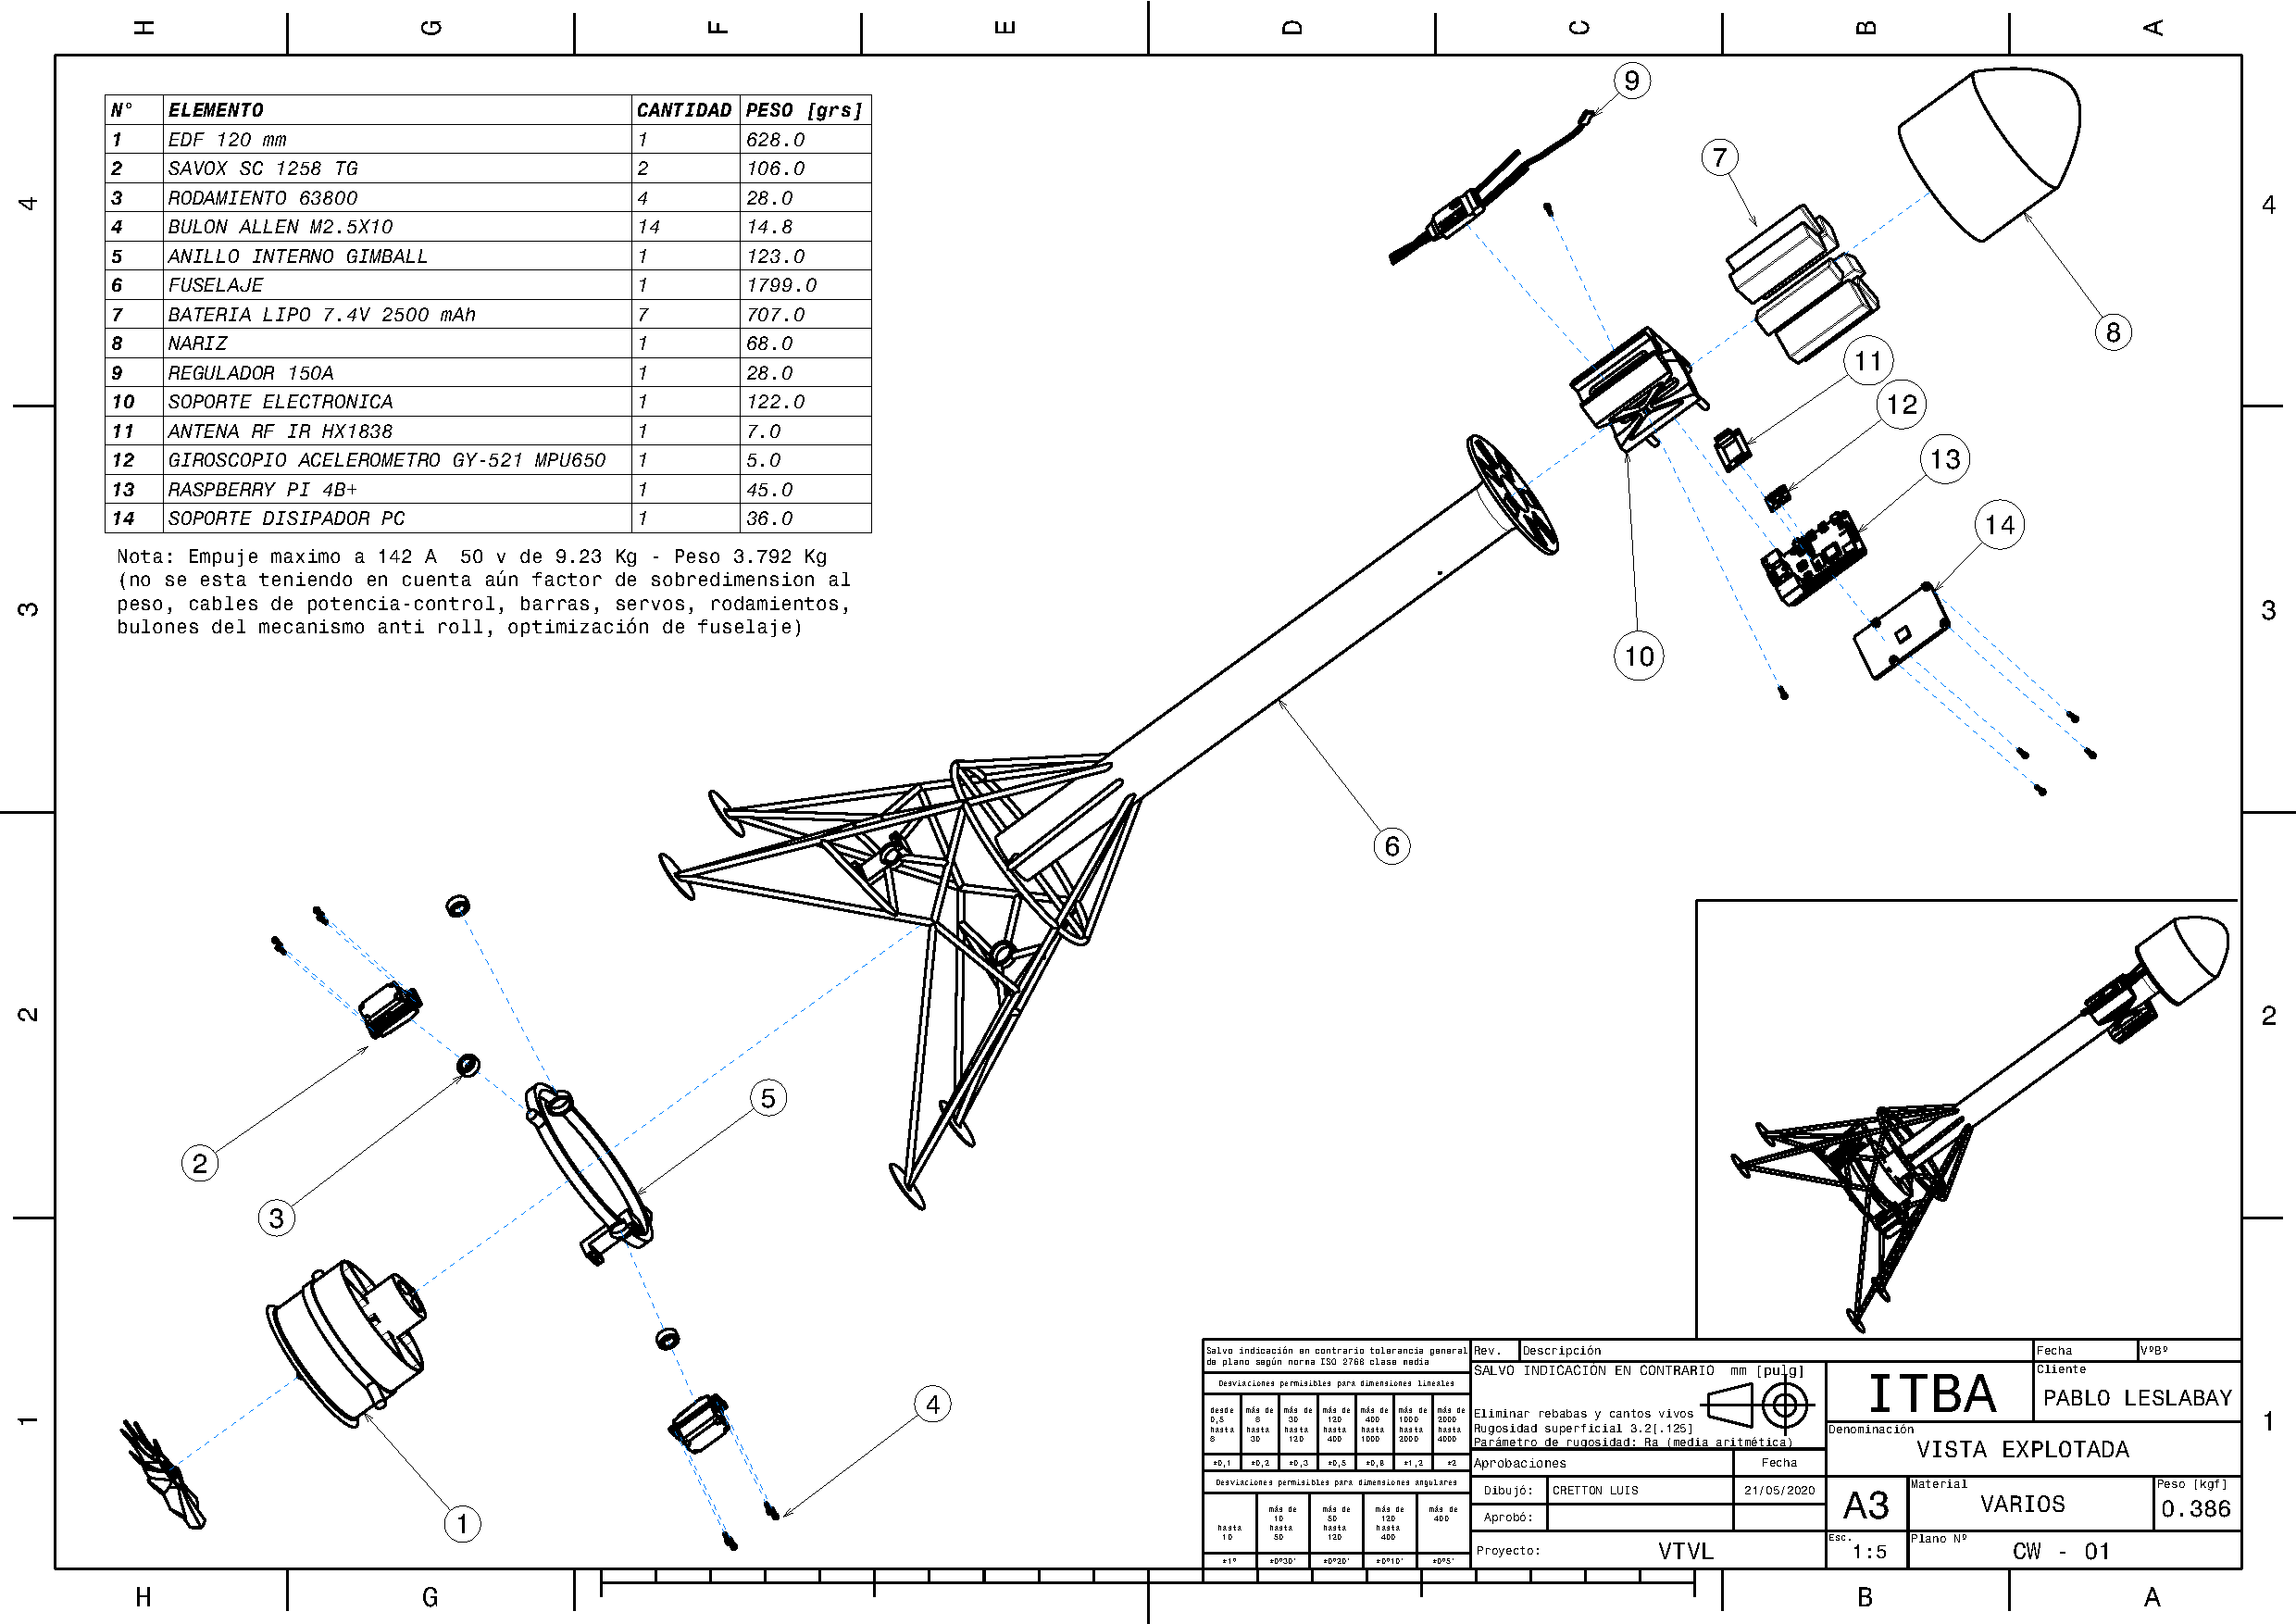
\includepdf[angle=90]{pdf/cad/Vista explotada 1.0}
\includepdf[angle=90]{pdf/cad/Vista explotada 5}


% VERSION FINAL
\section{Planos finales}
\includepdf[angle=90]{pdf/cad/ALUM-06-01}
\includepdf[angle=90]{pdf/cad/ALUM-06-02}
\includepdf[angle=90]{pdf/cad/ALUM-06-03}
\includepdf[angle=0]{pdf/cad/ALUM-06-04}
\includepdf[angle=0]{pdf/cad/ALUM-06-05}
\includepdf[angle=0]{pdf/cad/ALUM-06-06}
\includepdf[angle=0]{pdf/cad/ALUM-06-07}
\includepdf[angle=0]{pdf/cad/ALUM-06-08}
\includepdf[angle=0]{pdf/cad/ALUM-06-09}
\includepdf[angle=0]{pdf/cad/ALUM-06-10}
\includepdf[angle=0]{pdf/cad/ALUM-06-11}
\includepdf[angle=0]{pdf/cad/ALUM-06-12}
\includepdf[angle=0]{pdf/cad/ALUM-06-13}
\includepdf[angle=0]{pdf/cad/ALUM-06-14}
\includepdf[angle=0]{pdf/cad/ALUM-06-15}
\includepdf[angle=0]{pdf/cad/ALUM-06-16}

% \section{Dibujos de }

% \includepdf[angle=90]{pdf/cad/Vista explotada 1.0}



\end{document}
